% BEGIN INCLUDED SGA7I_English_current_buildable_source_20260823/components/128_expose_IX_title_and_contents.tex
% R2 explicit source correction R2-IX-06; see qa/FIDELITY-R2-CHANGES.json.
% SOURCE AUTHORITY:
% expose_IX_body.tex lines 5--64; scan indices 324--325; source folios 313--314.
% Direct scan comparison: physical PDF pages 325--326 at 1100 dpi.
% Hard stop before Introduction 0, source line 65.

\begin{center}
\SGARefAliasTarget{sga7.sga7i.eix.nroot}SGA 7

\vspace{1em}
\underline{报告 IX}

\vspace{1em}
\CJKunderdblline{N\'eron 模型与单值性}

\vspace{1em}
\underline{A. Grothendieck}

（附 M. Raynaud 的附录）
\end{center}

\subsection*{目录}

\begin{enumerate}[label=\arabic*.]
\setcounter{enumi}{-1}
\item 引言
\item 阿贝尔概形的 N\'eron 模型：记号；典范配对
  $\Phi_o\times\Phi'_o\longrightarrow(\mathbb Q/\mathbb Z)_k$，以及
  $(A^o,{A'}^o)$ 的典范双扩张 $W^o$
\item $T_\ell(A_K)$ 的不变部分与环面部分。良约化判据。
  $\ell\ne p$ 时的正交定理
\item 半稳定约化的情形。半稳定约化定理
\item 对 Serre--Tate 猜想及导子的应用
\item $\ell=p$ 时的正交定理（半稳定情形）。阿贝尔概形 $B_o$ 与 $B'_o$ 的对偶性。
  不变部分的刻画。良约化、本性良约化及半稳定约化的判据
\item 关于非半稳定约化情形中 $T_p(A)$ 的环面部分与不变部分的构造的注记
\item 与具有半稳定约化的阿贝尔概形 $A_K$ 相联系的 $S$ 上的 Raynaud 扩张
  $G^\natural$。$S$ 上的阿贝尔概形 $B,B'$ 的对偶性
\item 非半稳定情形中的 Raynaud 扩张 $A_K^{\natural\,o}$，以及 ind-群 $A_K^\natural$
\item 单值配对
  $\underline M_\ell\otimes\underline M'_\ell\longrightarrow
  \mathbb Z_{\ell S}$ 的定义
\item 单值配对的性质。整性与正性定理
\item N\'eron 模型的连通分支：对偶关系与渐近行为
\item Jacobian 的 N\'eron 模型与 Picard--Lefschetz 公式
\item 与超越理论的关系：复解析情形
  \begin{enumerate}[label=\arabic{enumi}.\arabic*.]
  \item $S$ 上解析群的回顾
  \item 沿一条纤维的形式完备化
  \item 解析的 Raynaud 扩张
  \item 用 Deligne 的“混合 Hodge 结构”作出的解释
  \item 相对代数情形
  \end{enumerate}
\item 与超越理论的关系：刚性解析情形。典范同态
  $\underline M_K\longrightarrow A_K^{\natural\,o}$
\end{enumerate}


% END INCLUDED SGA7I_English_current_buildable_source_20260823/components/128_expose_IX_title_and_contents.tex

% BEGIN INCLUDED SGA7I_English_current_buildable_source_20260823/components/129_expose_IX_introduction_and_leitfaden.tex
% SOURCE AUTHORITY:
% expose_IX_body.tex lines 65--140; scan indices 325--329; source folios 314--318.
% Direct scan comparison: physical PDF pages 326--330 at 1100 dpi.
% Leitfaden checked from four direct-source crops at 5000 dpi; all 18 strokes
% are plain, unlabelled, undirected segments. Hard stop before source line 144.

0. \underline{引言}

\SGARefTarget{sga7.sga7i.eix.n0-1}{0.1}. 本讲将前几讲的结果用于研究定义在 Hensel 性状 $S$ 的函数域 $K$ 上的阿贝尔概形 $A_K$ 的
\underline{N\'eron 模型}（\SGARefLink{sga7.sga7i.eix.n1-1}{1.1}）$A$。
我们将看到，N\'eron 模型最重要的性质都可以用局部单值群 $I$ 在 Tate 模
$T_\ell(A_K(\overline K))$ 上的作用来解释（其中 $\ell$ 是不同于 $p$ 的素数）。
由于后者的对偶可解释为 $\ell$ 进上同调群 $H^1(A_{\overline K},\mathbb Z_\ell)$，
而且对于任意 $K$ 上的光滑射影概形 $X$，$H^1(X_{\overline K},\mathbb Z_\ell)$
可与 $H^1(A_{\overline K},\mathbb Z_\ell)$ 等同，其中 $A_{\overline K}$ 是
$X_{\overline K}$ 的 Albanese 簇，所以本讲也可看作对
\underline{$K$ 上光滑射影簇的 $\ell$ 进 $H^1$ 的局部单值现象}
（更确切地说，是“动机”$H^1$ 的局部单值现象）的详细研究。
从这一观点看，本讲的主要结果显然应当包含在任意权动机的“N\'eron 理论”之中，
也就是任意 $i$ 的 $H^i$（$\ell$ 进、de Rham、Hodge 等）的理论之中；
目前，我们才刚刚开始窥见这种理论的轮廓。（有关这一点，参看 [9]，尤其是该报告中 Deligne 的猜想 9.8 至 9.13。）

\SGARefTarget{sga7.sga7i.eix.n0-2}{0.2}. 本讲最重要的结果是“\underline{半稳定约化定理}”\SGARefLink{sga7.sga7i.eix.n3-6}{3.6}。
它断言：对 $K$ 作一个有限可分扩张 $K'$ 后，$A_{K'}$ 的 N\'eron 模型的特殊纤维的单位连通分支，
是一个阿贝尔概形被一个环面的扩张。J.-P. Serre 于 1964 年提出了这一猜想，
这里给出的证明的基本思路\footnote{这一思路详述于报告人 1964 年 10 月 30 日致 J.-P. Serre 的信中。}
也始于同年。\SGARefLink{sga7.sga7i.eix.n3-5}{3.5} 将表明，这一“半稳定约化”性质，
等价于单值群 $I$ 在 $T_\ell(A_K(\overline K))$ 上的作用是“本性地二阶幺幂的”
（其中 $\ell$ 是一个固定的、不同于 $S$ 的剩余特征 $p$ 的素数）。
在第 III 讲中，利用 $2$ 维优良概形的奇点消解（由 S. Abhyankar 给出），
已经以 $\ell$ 进 $H^1$ 的语言证明了这一形式的断言，作为“\underline{单值性定理}”的特例。
要证明上述两种性质的等价性，我们还需要一个“正交定理”\SGARefLink{sga7.sga7i.eix.n2-4}{2.4}。
在 $A_K$ 是 $K$ 上光滑曲线 $X_K$ 的 Jacobian，而该曲线是 $S$ 上某个正则连通射影概形 $X$ 的一般纤维，
其几何特殊纤维只有普通二次奇点这一特殊情形下，该定理由 Igusa [11] 给出。
这确实是半稳定约化的一种情形，但不足以满足我们的需要；
我们采用前两讲所发展的双扩张理论这一便利工具，主要就是为了建立一般形式的正交定理。
还要指出，D. Mumford 找到了半稳定约化定理的另一种截然不同的证明：
它不使用奇点消解，而使用他的 theta 函数理论（未发表）；遗憾的是，他必须将剩余特征限制为不同于 $2$。

\SGARefTarget{sga7.sga7i.eix.n0-3}{0.3}. 在以后各节中，半稳定约化定理是研究 N\'eron 模型的主要工具；
这里的研究采用\underline{“代数”观点}。从\underline{“刚性解析”观点}，
或者从“theta 函数”的观点研究 $K$ 上的阿贝尔簇时，这一定理看来同样不可或缺
（对于完备赋值域上的阿贝尔簇，这两个术语似乎是同义的）。
后一观点由 D. Mumford 和 M. Raynaud 继 Tate 和 Morikawa 的工作之后于近年发展起来。
（第 13、14 节将略述代数观点与超越观点的关系。）
最后，同一定理还是 Artin--Deligne--Mumford 的“\underline{代数曲线的半稳定约化定理}”[3]
的证明中的一个关键要素；\footnote{P. Deligne 在讨论班的口头报告中给出了这一定理的证明，但当时认为没有必要将其收入讨论班文稿。}
研究单值性在基本群上的作用时（第 V 讲的“本性温和作用定理”），我们已经用过这一曲线定理，
而本讲整性与正性定理 \SGARefLink{sga7.sga7i.eix.n10-4}{10.4} 的证明还会再次用到它。
\footnote{后一条定理还有一种经由刚性解析理论的证明，不使用半稳定约化定理。}

\SGARefTarget{sga7.sga7i.eix.n0-4}{0.4}. 本讲与讨论班的其他各讲有所不同：
研究 Tate 模 $T_\ell(A_K)$ 时，我们也系统地考虑了 $\ell$ 等于剩余特征 $p$ 的情形。
事实表明，\underline{Barsotti--Tate 群} [33]\footnote{按 Tate 的术语，也称“$p$ 可除群”。}
的语言，使得 $\ell\ne p$ 时所建立的所有最重要的现象都能推广到这一情形；
有时需要用到 Tate 的基本定理 [33，定理 4]，而目前该定理只在 $K$ 为零特征时才得到证明。
当然，在后一情形中，pro-$p$ Barsotti--Tate 群 $T_p(A_K)$ 仍可解释为单值群 $I$ 在
$p$ 进模 $T_p(A_K(\overline K))$ 上的作用，
但应当注意，由它与 $\ell\ne p$ 情形的这种表面类比所提示的大多数命题，都是完全错误的。
（例如，当 $\ell=p$ 时，单值作用不再一定是本性幺幂的。）
然而，只要作出更恰当的转述（如下文 \SGARefLink{sga7.sga7i.eix.n5-13}{5.13}），就已经可以清楚地看出：
定义在剩余特征 $p>0$ 的性状的函数域上、具有几何来源的 pro-$p$ Barsotti--Tate 群，
无论该性状是否为混合特征，其研究都应视作“局部单值性”理论的一部分；
这些群在这一理论中扮演 $\operatorname{Spec}(K)$ 上的\underline{$p$ 进局部系统}的角色。
实际上，从\underline{“$p$ 进”观点研究 $K$ 上光滑射影簇的 $H^1$} 时，所出现的“局部系统”本质上正是这些群。
若要从 $p$ 进观点研究更高次的 $H^i$——这一研究尚待开展——
看来必须适当扩充 $K$ 上、分别 $S$ 上的 pro-$p$ Barsotti--Tate 群范畴，
并从“晶体上同调”所提供的观点中汲取启发。

\SGARefTarget{sga7.sga7i.eix.n0-5}{0.5}. 这里给出的文稿直到第 4 节都与口头报告十分接近，
但从以后各节开始，内容明显更为详尽和完整；这些部分在口头报告中只作了部分勾勒。
后面的各讲将不使用本讲。另一方面，本讲的一些结果
（\SGARefLink{sga7.sga7i.eix.n10-4}{10.4} 和 \SGARefLink{sga7.sga7i.eix.n12-5}{12.5}）
使用了以后才会建立的\underline{Picard--Lefschetz 公式}。

\begin{center}
\underline{阅读路线图}

\vspace{0.5em}
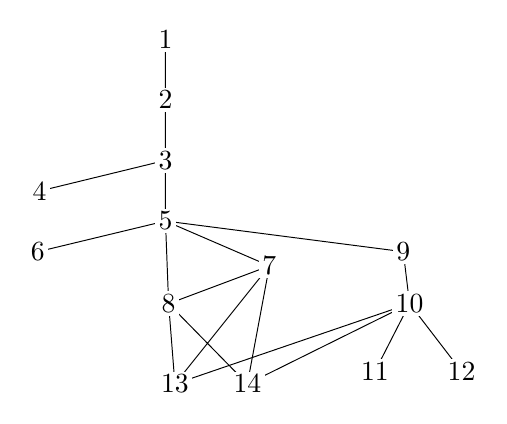
\begin{tikzpicture}[line width=0.35pt,every node/.style={fill=white,inner sep=1.2pt}]
  \coordinate (p1)  at ( 0.00, 0.00);
  \coordinate (p2)  at ( 0.00,-0.76);
  \coordinate (p3)  at ( 0.00,-1.53);
  \coordinate (p4)  at (-1.60,-1.92);
  \coordinate (p5)  at ( 0.00,-2.30);
  \coordinate (p6)  at (-1.62,-2.69);
  \coordinate (p7)  at ( 1.32,-2.87);
  \coordinate (p8)  at ( 0.04,-3.35);
  \coordinate (p9)  at ( 3.02,-2.69);
  \coordinate (p10) at ( 3.10,-3.35);
  \coordinate (p11) at ( 2.66,-4.21);
  \coordinate (p12) at ( 3.76,-4.21);
  \coordinate (p13) at ( 0.12,-4.37);
  \coordinate (p14) at ( 1.04,-4.37);
  \draw (p1)--(p2) (p2)--(p3) (p3)--(p4) (p3)--(p5)
        (p5)--(p6) (p5)--(p7) (p5)--(p8) (p5)--(p9)
        (p7)--(p8) (p7)--(p13) (p7)--(p14)
        (p8)--(p13) (p8)--(p14) (p9)--(p10)
        (p10)--(p11) (p10)--(p12) (p10)--(p13) (p10)--(p14);
  \node at (p1)  {1};  \node at (p2)  {2};
  \node at (p3)  {3};  \node at (p4)  {4};
  \node at (p5)  {5};  \node at (p6)  {6};
  \node at (p7)  {7};  \node at (p8)  {8};
  \node at (p9)  {9};  \node at (p10) {10};
  \node at (p11) {11}; \node at (p12) {12};
  \node at (p13) {13}; \node at (p14) {14};
\end{tikzpicture}
\end{center}


% END INCLUDED SGA7I_English_current_buildable_source_20260823/components/129_expose_IX_introduction_and_leitfaden.tex

% BEGIN INCLUDED SGA7I_English_current_buildable_source_20260823/components/130_expose_IX_section_1_0_and_1_1.tex
% Expose IX, 1.0--1.1.
% French transcription lines 144--260; authority scan physical pp. 331--334
% (source folios 319--322).  Ordinary pages were checked in four overlapping
% 1100-dpi bands.  The missing prime on A'_o in the final sentence of 1.1 is
% an ordinary printed/source slip and is restored below.

\medskip
\noindent
\underline{1. 阿贝尔概形的 N\'eron 模型：记号；典范配对}
\[
 \Phi_o\times\Phi'_o\longrightarrow(\mathbb Q/\mathbb Z)_k,
\]
\underline{以及 $(A^o,{A'}^o)$ 的典范双扩张 $W^o$。}

\medskip
\noindent
\SGARefTarget{sga7.sga7i.eix.n1-0}{1.0}. 本讲始终固定一个性状 $S$，并对它使用 I~1 中的通常记号
$s$、$\eta$、$k$、$K$ 等。设 $A_K$ 是 $K$ 上的一个阿贝尔概形，
将其对偶阿贝尔概形 [5] 记为 $A'_K$。
$A_K$ 与 $A'_K$ 之间的对偶性由 $(A_K,A'_K)$ 上的一个除子对应 $W_K$ 给出，
也就是 $A_K\times A'_K$ 上相对于 $A_K$ 和 $A'_K$ 的单位截面双刚化的一个可逆层。
它由其类决定，精确到唯一同构（参见 VIII~\SGARefLink{sga7.sga7i.eviii.n3-1}{3.1}）：
\begin{equation}\tag{\SGARefTarget{sga7.sga7i.eix.n1-0-1}{1.0.1}}
 w_K\in\mathrm{Biext}^1(A_K,A'_K;\mathbb G_{mK}).
\end{equation}
相应的配对（VIII~\SGARefLink{sga7.sga7i.eviii.n2-2}{2.2}）将起重要作用：
\begin{equation}\tag{\SGARefTarget{sga7.sga7i.eix.n1-0-2}{1.0.2}}
 \varphi:T_\ell(A_K)\times T_\ell(A'_K)
 \longrightarrow\mathbb Z_\ell(1)_K
 \overset{\mathrm{def}}{=}T_\ell(\mathbb G_{mK}),
\end{equation}
其中 $\ell$ 是任意素数。当 $\ell\ne p=\operatorname{char}k$ 时，
给定 $\varphi$ 等价于给定有限自由 $\mathbb Z_\ell$ 模的配对
\begin{equation}\tag{\SGARefTarget{sga7.sga7i.eix.n1-0-3}{1.0.3}}
 \varphi:T_\ell(A_K(\overline K))\times
 T_\ell(A'_K(\overline K))\longrightarrow T_\ell(\overline K^*),
\end{equation}
它与
\[
 \pi=\operatorname{Gal}(\overline K/K)
\]
在上述三个模上的作用相容，其中 $\overline K$ 是 $K$ 的一个可分闭包。
已知（VIII~\SGARefLink{sga7.sga7i.eviii.n3-2}{3.2}）这一配对是完美对偶（perfect duality）：
它将 $T_\ell(A_K(\overline K))$ 与 $T_\ell(A'_K(\overline K))$ 中的每一个模，
与另一个模的取值于可逆模 $\mathbb Z_\ell(1)=T_\ell(\overline K^*)$ 的对偶等同。

有时我们假定已经选定 $A_K$ 的一个极化（polarization）；也就是说，给定一个元素
\begin{equation}\tag{\SGARefTarget{sga7.sga7i.eix.n1-0-4}{1.0.4}}
 \xi\in\operatorname{NS}(A_K/K)
 =\underline{\operatorname{NS}}_{A_K/K}(K),
\end{equation}
其中
\[
 \underline{\operatorname{NS}}_{A_K/K}
 \overset{\mathrm{def}}{=}
 \underline{\operatorname{Pic}}_{A_K/K}/
 \bigl(\underline{\operatorname{Pic}}{}^o_{A_K/K}=A'_K\bigr).
\]
它按通常的方式定义同态
\begin{equation}\tag{\SGARefTarget{sga7.sga7i.eix.n1-0-5}{1.0.5}}
 \psi_\xi:A_K\longrightarrow A'_K,
\end{equation}
从而定义同态
\begin{equation}\tag{\SGARefTarget{sga7.sga7i.eix.n1-0-6}{1.0.6}}
 T_\ell(\psi_\xi),\quad\text{或简记为}\quad
 \psi_\xi:T_\ell(A_K)\longrightarrow T_\ell(A'_K),
\end{equation}
以及双线性形式 $\varphi_\xi$
\begin{equation}\tag{\SGARefTarget{sga7.sga7i.eix.n1-0-7}{1.0.7}}
 \begin{split}
 \varphi_\xi(x,y)&=\varphi(x,\psi_\xi(y)),\\
 \varphi_\xi:T_\ell(A_K)\times T_\ell(A_K)
 &\longrightarrow\mathbb Z_\ell(1)_K,
 \end{split}
\end{equation}
当 $\ell\ne p$ 时，它也可解释为带算子的有限自由 $\mathbb Z_\ell$ 模的配对：
\begin{equation}\tag{\SGARefTarget{sga7.sga7i.eix.n1-0-8}{1.0.8}}
 \varphi_\xi:T_\ell(A_K(\overline K))\times
 T_\ell(A_K(\overline K))\longrightarrow T_\ell(\overline K^*).
\end{equation}
上述构造对 $A_K$ 的 N\'eron--Severi 群中的每个元素都有意义，
而且无论采用解释（\SGARefLink{sga7.sga7i.eix.n1-0-7}{1.0.7}）还是（\SGARefLink{sga7.sga7i.eix.n1-0-8}{1.0.8}），
得到的形式 $\varphi_\xi$ 都是\underline{交替的}（VIII~\SGARefLink{sga7.sga7i.eviii.n2-2-11}{2.2.11}）。
$\xi$ 是一个\underline{极化}这一事实，意味着（\SGARefLink{sga7.sga7i.eix.n1-0-5}{1.0.5}）中的 $\psi_\xi$ 是一个同源（isogeny）；等价地，由于 $\dim A_K=\dim A'_K$，它是群的满态射。
这也等价于（\SGARefLink{sga7.sga7i.eix.n1-0-6}{1.0.6}）中的 $T_\ell(\psi_\xi)$ 为单射
（或者等价于其余核有限），最后还等价于（\SGARefLink{sga7.sga7i.eix.n1-0-7}{1.0.7}）中的形式 $\varphi_\xi$
是\underline{分离的}（separating）。

\medskip
\noindent
\SGARefTarget{sga7.sga7i.eix.n1-1}{1.1}. 回顾一下，存在一个 $S$ 上的\underline{光滑概形} $A$，
称为 \underline{$A_K$ 的 N\'eron 模型}，它在光滑 $S$ 概形的范畴上表示函子
\begin{equation}\tag{\SGARefTarget{sga7.sga7i.eix.n1-1-1}{1.1.1}}
 S'\longmapsto\operatorname{Hom}(S'_\eta,A_K)
\end{equation}
因此，按定义，对光滑相对 $S$ 概形 $S'$ 有函子性的同构
\begin{equation}\tag{\SGARefTarget{sga7.sga7i.eix.n1-1-2}{1.1.2}}
 \operatorname{Hom}_S(S',A)\simeq
 \operatorname{Hom}_K(S'_\eta,A_K).
\end{equation}
当 $S$ 的剩余域 $k$ 完美时，N\'eron [19] 构造了 $A$。
Raynaud 在 1966--67 年于 IHES 举行的一个未成文的讨论班中，
把这一构造推广到一般情形（Raynaud 的主要结果陈述见 [21]，它们补全了 N\'eron 在上述文献中的结果）。
这里将不加证明地使用这一存在性结果，以及 $A$ 是 $S$ 上的拟射影\underline{概形}这一事实。
当 $S'$ 光滑\underline{于} $\eta$ 上时应用（\SGARefLink{sga7.sga7i.eix.n1-1-2}{1.1.2}），
还可得到下面的典范态射是同构：
\begin{equation}\tag{\SGARefTarget{sga7.sga7i.eix.n1-1-3}{1.1.3}}
 A\times_S\operatorname{Spec}(K)\xrightarrow{\ \sim\ }A_K.
\end{equation}
这就说明了配套记号 $A,A_K$ 的合理性；方便时也将 $A_K$ 写成 $A_\eta$。
用（\SGARefLink{sga7.sga7i.eix.n1-1-3}{1.1.3}）作等同同构后，
典范双射（\SGARefLink{sga7.sga7i.eix.n1-1-2}{1.1.2}）就是\underline{限制到一般纤维}所给出的映射。

由于函子（\SGARefLink{sga7.sga7i.eix.n1-1-1}{1.1.1}）显然带有交换群结构，
表示它的 N\'eron 模型 $A$ 本身也带有 \underline{$S$ 上的光滑交换群概形}结构。
本讲其余部分将研究这一群概形。

由 N\'eron 模型产生的一个重要不变量，当然是 $k$ 上的有限型光滑交换群概形
\begin{equation}\tag{\SGARefTarget{sga7.sga7i.eix.n1-1-4}{1.1.4}}
 A_o=A\times_Ss=A_k.
\end{equation}
依照一般记号，将它的单位连通分支记为 $A_o^o$，并考虑群概形
\begin{equation}\tag{\SGARefTarget{sga7.sga7i.eix.n1-1-5}{1.1.5}}
 \Phi_o=A_o/A_o^o
\end{equation}
它是 $A_o$ 的连通分支群，在 $k$ 上有限且平展。因此，取 $k$ 的一个可分闭包 $\overline k$，
它由通常意义下的有限群
\begin{equation}\tag{\SGARefTarget{sga7.sga7i.eix.n1-1-6}{1.1.6}}
 \Phi_o(\overline k),
\end{equation}
以及
\[
 \pi_o=\operatorname{Gal}(\overline k/k)
\]
在该群上的自然作用所决定。

在研究 $A_K$ 的 N\'eron 模型 $A$ 的同时，我们还将研究
\begin{equation}\tag{\SGARefTarget{sga7.sga7i.eix.n1-1-7}{1.1.7}}
 A'=\text{概形 }A'_K\text{ 的 N\'eron 模型},
\end{equation}
它同样是 $S$ 上的有限型光滑交换群概形。我们以
\begin{equation}\tag{\SGARefTarget{sga7.sga7i.eix.n1-1-8}{1.1.8}}
 \Phi'_o=A'_o/{A'}_o^o
\end{equation}
表示其特殊纤维 $A'_o$ 的连通分支群。

% END INCLUDED SGA7I_English_current_buildable_source_20260823/components/130_expose_IX_section_1_0_and_1_1.tex

% BEGIN INCLUDED SGA7I_English_current_buildable_source_20260823/components/131_expose_IX_sections_1_2_through_1_5.tex
% Expose IX, 1.2--1.5.
% French transcription lines 265--341; authority scan physical pp. 335--338
% (source folios 323--326).  Ordinary pages were checked in four overlapping
% 1100-dpi bands.  Formula (1.4.2) was checked in targeted 5000-dpi crops.

\medskip
\noindent
\SGARefTarget{sga7.sga7i.eix.n1-2}{1.2}. 对 $(A,A')$ 这一偶以及（\SGARefLink{sga7.sga7i.eix.n1-0-1}{1.0.1}）中
$(A_K,A'_K)$ 被 $\mathbb G_{mK}$ 的双扩张 $W_K$ 应用 VIII~\SGARefLink{sga7.sga7i.eviii.n7-1}{7.1}(b)，
便得到一个\underline{典范配对}
\begin{equation}\tag{\SGARefTarget{sga7.sga7i.eix.n1-2-1}{1.2.1}}
 \Phi_o\times\Phi'_o\longrightarrow(\mathbb Q/\mathbb Z)_k,
\end{equation}
也就是 $\pi_o$ 模的配对
\begin{equation}\tag{\SGARefTarget{sga7.sga7i.eix.n1-2-2}{1.2.2}}
 \Phi_o(\overline k)\times\Phi'_o(\overline k)
 \longrightarrow\mathbb Q/\mathbb Z.
\end{equation}
这里，此配对表现为将 $W_K$ 延拓为 $(A,A')$ 被 $\mathbb G_{mS}$ 的双扩张 $W$ 的障碍；
这一观点的含义在 VIII~\SGARefLink{sga7.sga7i.eviii.n7-3-2}{7.3.2} 中已有解释。
我们立即记下关于这个配对的如下猜想。

\medskip
\noindent
\underline{猜想 \SGARefTarget{sga7.sga7i.eix.n1-3}{1.3}。}
\underline{配对}（\SGARefLink{sga7.sga7i.eix.n1-2-1}{1.2.1}）\underline{是完美对偶}：
\underline{它将分支群} $\Phi_o$ \underline{和} $\Phi'_o$ \underline{中的每一个与另一个的取值于}
$(\mathbb Q/\mathbb Z)_k$ \underline{的对偶等同}。

\medskip
\noindent
\SGARefTarget{sga7.sga7i.eix.n1-3-1}{1.3.1}. 配对（\SGARefLink{sga7.sga7i.eix.n1-2-1}{1.2.1}）的形成与形式平展基变换交换
（VIII~\SGARefLink{sga7.sga7i.eviii.n7-3-5-3}{7.3.5.3}），N\'eron 模型的形成也有类似性质。
因此，要证明猜想~\SGARefLink{sga7.sga7i.eix.n1-3}{1.3}，只须处理 $S$ 完备且剩余域可分闭的情形。
当 $A_K$ 是 $K$ 上一条紧合光滑曲线的 Jacobian 时，Artin 和 Mazur 已经证明了这一猜想，
他们使用了自己的关于 $S$ 上紧合曲线概形的相对 Jacobian 的自对偶性（在导出范畴意义下）的一般理论；该理论尚未发表。
他们还利用 Tate 对偶性 [32]，证明了剩余域为\underline{有限域}时的猜想~\SGARefLink{sga7.sga7i.eix.n1-3}{1.3}。
我们也将在 \SGARefLink{sga7.sga7i.eix.n11-4}{11.4} 和 \SGARefLink{sga7.sga7i.eix.n11-5}{11.5} 中看到
（尚须核对相容性），\SGARefLink{sga7.sga7i.eix.n1-3}{1.3} 对 $\ell\ne p$ 的 $\ell$ 准素部分成立，
而且在“半稳定约化”情形下成立。这些结果使 \SGARefLink{sga7.sga7i.eix.n1-3}{1.3} 极为可信。
此外，也可将 \SGARefLink{sga7.sga7i.eix.n1-3}{1.3} 看成完备离散赋值环的分式域上的群概形的一般对偶理论的一个副产品，
该理论在形式上类似于 SGA~5~I。目前，这样的理论仍处于探索阶段；
它还应包含 Serre [27] 所给形式的局部类域论。

\medskip
\noindent
\SGARefTarget{sga7.sga7i.eix.n1-3-2}{1.3.2}. 对给定阿贝尔概形 $A_K$，
\SGARefLink{sga7.sga7i.eix.n1-3}{1.3} 成立意味着配对（\SGARefLink{sga7.sga7i.eix.n1-2-1}{1.2.1}）
在左右两侧都是\underline{分离的}。由 VIII~\SGARefLink{sga7.sga7i.eviii.n7-3-2}{7.3.2}，
左侧的分离性恰好意味着：$A$ 的开子群概形 $V$ 中，
使 $W_K$ 可延拓为 $(V,A')$ 被 $\mathbb G_{mS}$ 的双扩张的，只有 $A$ 的单位连通分支 $A^o$。
右侧的分离性也有对称的解释。

\medskip
\noindent
\SGARefTarget{sga7.sga7i.eix.n1-4}{1.4}. 更一般地，设
\begin{equation}\tag{\SGARefTarget{sga7.sga7i.eix.n1-4-1}{1.4.1}}
 U\subset A\qquad\text{和}\qquad U'\subset A'
\end{equation}
是开子群概形，并使得 $W_K$ 可延拓为 $(U,U')$ 被 $\mathbb G_{mS}$ 的双扩张。
由 VIII~\SGARefLink{sga7.sga7i.eviii.n7-3-2}{7.3.2}，这具体地说就是，
由 $U$ 和 $U'$ 所定义的子群
% SGA-SRC-001266
\begin{equation}\tag{\SGARefTarget{sga7.sga7i.eix.n1-4-2}{1.4.2}}
 F_o=U_o/U_o^o\subset\Phi_o,
 \qquad
 F'_o=U'_o/{U'}_o^o\subset\Phi'_o
\end{equation}
在（\SGARefLink{sga7.sga7i.eix.n1-2-1}{1.2.1}）下正交。
\footnote{印本公式经直接高分辨率核对，确实将 $\Phi'_o$ 重复用于第一个子群，
并将第二个子群写成 $\Psi'_o\subset\Psi_o$，这与已经确定的 $A'$ 的分支群记号冲突。
上述中性的局部记号 $F_o,F'_o$ 使所指的两个子群明确无歧义，而不改变命题。}
将 $W_K$ 的这一延拓（精确到唯一同构是唯一的）记为 $W$。
它由其类决定，精确到唯一同构：
\begin{equation}\tag{\SGARefTarget{sga7.sga7i.eix.n1-4-3}{1.4.3}}
 w\in\mathrm{Biext}^1(U,U';\mathbb G_{mS}),
\end{equation}
该类本身则由如下条件刻画：它在 $\mathrm{Biext}^1(A_K,A'_K;\mathbb G_{mK})$ 中的像
是（\SGARefLink{sga7.sga7i.eix.n1-0-1}{1.0.1}）中的类 $w_K$。

例如，可以取 $U$ 和 $U'$ 为 $A$ 和 $A'$ 的单位连通分支 $A^o$ 和 $A'{}^o$。
由此得到 \underline{$(A^o,A'{}^o)$ 被 $\mathbb G_{mS}$ 的典范双扩张 $W^o$，或记为 $W$}，
它给出一个类
\begin{equation}\tag{\SGARefTarget{sga7.sga7i.eix.n1-4-4}{1.4.4}}
 w=w^o\in\mathrm{Biext}^1(A^o,A'{}^o;\mathbb G_{mS}),
\end{equation}
我们主要研究这一类。显然，对不同的偶 $(U,U')$，
（\SGARefLink{sga7.sga7i.eix.n1-4-3}{1.4.3}）中的类 $w$ 在 $(A^o,A'{}^o)$ 上的限制，
都等于（\SGARefLink{sga7.sga7i.eix.n1-4-4}{1.4.4}）中的 $w^o$。

\medskip
\noindent
\underline{命题 \SGARefTarget{sga7.sga7i.eix.n1-5}{1.5}。}
\underline{考虑（\SGARefLink{sga7.sga7i.eix.n1-4-4}{1.4.4}）中 $(A^o,A'{}^o)$ 被 $\mathbb G_{mS}$ 的典范双扩张 $W$ 的特殊纤维 $W_s$；
因而 $W_s$ 是 $(A_o^o,{A'}_o^o)$ 被 $\mathbb G_{mk}$ 的双扩张。这个双扩张是分离的}
（VIII~\SGARefLink{sga7.sga7i.eviii.n4-11}{4.11}）。

事实上，在 $A^o$ 上选取一个丰沛可逆层 $\mathbb L$。于是 $\mathbb L_\eta$ 定义同态
（参见 \SGARefLink{sga7.sga7i.eix.n1-0-5}{1.0.5}）
\[
 A_K\longrightarrow A'_K,
\]
它延拓为同态 $A\longrightarrow A'$，从而给出
\[
 \psi:A^o\longrightarrow A'{}^o.
\]
考虑沿 $(\operatorname{id}_{A^o},\psi)$ 拉回 $W$ 所得到的
$(A^o,A^o)$ 被 $\mathbb G_{mS}$ 的双扩张 $W_{\mathbb L}$。
它在一般纤维上的限制，恰是 VIII~\SGARefLink{sga7.sga7i.eviii.n4-12}{4.12} 中的双扩张 $\delta(\mathbb L_\eta)$。
因此，由 VIII~\SGARefLink{sga7.sga7i.eviii.n7-4}{7.4}，$W_{\mathbb L}$ 与双刚化可逆层 $\delta(\mathbb L)$ 相联系，
从而 $(W_{\mathbb L})_s$ 由 $\delta(\mathbb L_s)$ 定义。
另一方面，它也可描述为由态射
\[
 \operatorname{id}_{A_o^o}:A_o^o\longrightarrow A_o^o,
 \qquad
 \psi_o:A_o^o\longrightarrow {A'}_o^o.
\]
拉回 $W_s$ 所得到的双扩张。
由于 $\mathbb L$ 丰沛，$\mathbb L_s$ 也丰沛，VIII~\SGARefLink{sga7.sga7i.eviii.n4-13}{4.13} 表明
$W_{\mathbb L_s}$ 是分离的，特别是在左侧分离。
于是 $W_s$ 更在左侧分离。由对称性，它在右侧也分离，这就证明了 \SGARefLink{sga7.sga7i.eix.n1-5}{1.5}。

当 $A_o^o$ 的幺幂秩为零时，我们将大幅加强 \SGARefLink{sga7.sga7i.eix.n1-5}{1.5}
（\SGARefLink{sga7.sga7i.eix.n5-4}{5.4}）。

% END INCLUDED SGA7I_English_current_buildable_source_20260823/components/131_expose_IX_sections_1_2_through_1_5.tex

% BEGIN INCLUDED SGA7I_English_current_buildable_source_20260823/components/132_expose_IX_section_2_1.tex
% Expose IX, section 2 title and 2.1--2.1.14.
% French transcription lines 344--441; authority physical pp. 338--341
% (source folios 326--329).  All pages were checked in four overlapping
% 1100-dpi bands.  Diagram (2.1.6) was checked node-by-node and arrow-by-arrow
% in four overlapping direct-source crops rendered at 5000 dpi.

\medskip
\noindent
\underline{2. $T_\ell(A_K)$ 的不变部分与环面部分。良约化判据。$\ell\ne p$ 时的正交定理。}

\medskip
\noindent
\SGARefTarget{sga7.sga7i.eix.n2-1}{2.1}. 与 $k$ 上的每个交换代数群一样，$A_o$ 有一个最大的子环面，
其形成与基域的任意扩张交换 [SGA~3 XVII~7.2.1，XII~1.12]：
\begin{equation}\tag{\SGARefTarget{sga7.sga7i.eix.n2-1-1}{2.1.1}}
 T_o\subset A_o.
\end{equation}
当 $k$ 完美时，$T_o$ 由如下条件刻画：$A_o^o/T_o$ 是 $k$ 上一个阿贝尔概形 $B_o$
被一个光滑连通幺幂群的扩张 [25]。
后者必有一个合成列，其所有商群都同构于 $\mathbb G_{ak}$（SGA~3 XVII~4.1.3），并且有正合列
\begin{equation}\tag{\SGARefTarget{sga7.sga7i.eix.n2-1-2}{2.1.2}}
 0\longrightarrow U_o\longrightarrow A_o^o/T_o
 \longrightarrow B_o\longrightarrow0.
\end{equation}
无论 $k$ 是否完美，\underline{如果} $A_o^o$ 是一个阿贝尔概形 $B_o$
被一个光滑连通仿射概形 $L_o$ 的扩张，
\begin{equation}\tag{\SGARefTarget{sga7.sga7i.eix.n2-1-3}{2.1.3}}
 0\longrightarrow L_o\longrightarrow A_o^o
 \longrightarrow B_o\longrightarrow0,
\end{equation}
则已知这一扩张结构是唯一的 [25]。
此外，$T_o\subset L_o$，且 $T_o$ 是 $L_o$ 的最大子环面。
因此，有正合列（\SGARefLink{sga7.sga7i.eix.n2-1-2}{2.1.2}），其中
\begin{equation}\tag{\SGARefTarget{sga7.sga7i.eix.n2-1-4}{2.1.4}}
 U_o=L_o/T_o.
\end{equation}

\medskip
\noindent
\SGARefTarget{sga7.sga7i.eix.n2-1-5}{2.1.5}. 注意，$A_o^o$ 的\underline{幺幂秩为零}
（即在扩张到 $k$ 的一个代数闭包后，没有同构于 $\mathbb G_a$ 的子群），
当且仅当 $A_o^o/T_o$ 是一个阿贝尔概形 $B_o$。
这时，前述假设成立且 $U_o=0$。

设 $\ell$ 是一个不同于 $k$ 的特征的素数，因而 $A_o^o$ 是 $\ell$ 可除的。
包含映射（\SGARefLink{sga7.sga7i.eix.n2-1-1}{2.1.1}）于是给出 pro-群概形的正合列：
\begin{equation}\tag{\SGARefTarget{sga7.sga7i.eix.n2-1-6}{2.1.6}}
\begin{tikzcd}[row sep=large,column sep=large]
0 \arrow[r] & T_\ell(T_o) \arrow[r]
 & T_\ell(A_o^o) \arrow[r] \arrow[d,"\wr"]
 & T_\ell(A_o^o/T_o) \arrow[r] \arrow[d,"\wr"] & 0\\
 & & T_\ell(A_o) & T_\ell(A_o/T_o) & {,}
\end{tikzcd}
\end{equation}
其中各项也可解释为扭常自由 $\ell$ 进层。
若存在正合列（\SGARefLink{sga7.sga7i.eix.n2-1-2}{2.1.2}）——例如 $k$ 完美，或 $A_o^o$ 的幺幂秩为零时——则有
\begin{equation}\tag{\SGARefTarget{sga7.sga7i.eix.n2-1-7}{2.1.7}}
 T_\ell(A_o^o/T_o)\xrightarrow{\ \sim\ }T_\ell(B_o),
\end{equation}
因而正合列（\SGARefLink{sga7.sga7i.eix.n2-1-6}{2.1.6}）成为
\begin{equation}\tag{\SGARefTarget{sga7.sga7i.eix.n2-1-8}{2.1.8}}
 0\longrightarrow T_\ell(T_o)\longrightarrow T_\ell(A_o^o)
 \longrightarrow T_\ell(B_o)\longrightarrow0.
\end{equation}
置
\begin{equation}\tag{\SGARefTarget{sga7.sga7i.eix.n2-1-9}{2.1.9}}
 n=\dim A_K=\dim A_o,\qquad
 \mu=\dim T_o,\qquad
 \lambda=\dim U_o,\qquad
 \alpha=\dim B_o.
\end{equation}
于是
\begin{equation}\tag{\SGARefTarget{sga7.sga7i.eix.n2-1-10}{2.1.10}}
 n=\mu+\lambda+\alpha,
\end{equation}
并且
\begin{equation}\tag{\SGARefTarget{sga7.sga7i.eix.n2-1-11}{2.1.11}}
 \left\{
 \begin{aligned}
 \operatorname{rank}T_\ell(T_o)&=\mu,&
 \operatorname{rank}T_\ell(A_o^o/T_o)
 &=\operatorname{rank}T_\ell(B_o)=2\alpha,\\
 \operatorname{rank}T_\ell(A_o^o)&=\mu+2\alpha.
 \end{aligned}
 \right.
\end{equation}
第二个等式是 Weil 的一个著名定理 [5，15]。

\medskip
\noindent
\SGARefTarget{sga7.sga7i.eix.n2-1-12}{2.1.12}. 即使不假定正合列（\SGARefLink{sga7.sga7i.eix.n2-1-2}{2.1.2}）存在，
通过扩张到 $k$ 的一个代数闭包，显然仍可定义整数 $n,\mu,\lambda,\alpha$。
它们分别称为 $A_o$ 的维数、\underline{$A_o$ 的约化秩}（等于 $T_o$ 的维数）、
\underline{$A_o$ 的幺幂秩}以及\underline{$A_o$ 的阿贝尔秩}。
它们仍满足（\SGARefLink{sga7.sga7i.eix.n2-1-10}{2.1.10}）和（\SGARefLink{sga7.sga7i.eix.n2-1-11}{2.1.11}），
但后一式须略去 $\operatorname{rank}T_\ell(B_o)$ 这一项。

\medskip
\noindent
\SGARefTarget{sga7.sga7i.eix.n2-1-13}{2.1.13}. 设 $k$ 的特征为 $p>0$，且 $A_o^o$ 为 $p$ 可除的，
等价地，其幺幂秩为零（参见 \SGARefLink{sga7.sga7i.eix.n2-1-5}{2.1.5}）。
这时也应考虑 pro-群 $T_p(A_o^o)$，它是一个 \underline{Barsotti--Tate 群}
（或按 [33] 的术语，一个\underline{$p$ 可除群}）。
正合列（\SGARefLink{sga7.sga7i.eix.n2-1-8}{2.1.8}）对 $\ell=p$ 仍然成立，
此时它是 Barsotti--Tate 群的正合列。这里 $\lambda=0$，因而
\begin{equation}\tag{\SGARefTarget{sga7.sga7i.eix.n2-1-13-1}{2.1.13.1}}
 n=\mu+\alpha.
\end{equation}
公式（\SGARefLink{sga7.sga7i.eix.n2-1-11}{2.1.11}）也仍然有效，
但须将秩解释为相应 Barsotti--Tate 群的秩（或“高度”）。

\medskip
\noindent
\SGARefTarget{sga7.sga7i.eix.n2-1-14}{2.1.14}. 对 ${A'}_o^o$，我们同样引入不变量
\[
 T'_o\subset {A'}_o^o,\qquad U'_o,\qquad B'_o,
\]
其中 $T'_o$ 是 ${A'}_o^o$ 的环面部分，$B'_o$ 是其阿贝尔部分
（特别是在 $k$ 完美或 ${A'}_o^o$ 的幺幂秩为零时有定义），$U'_o$ 是其幺幂部分
（例如在 $k$ 完美时有定义，或在 ${A'}_o^o$ 的幺幂秩为零时平凡地有定义）。
存在相应的形如（\SGARefLink{sga7.sga7i.eix.n2-1-6}{2.1.6}）或（\SGARefLink{sga7.sga7i.eix.n2-1-8}{2.1.8}）的正合列，这里不再重写。
也可仿照（\SGARefLink{sga7.sga7i.eix.n2-1-9}{2.1.9}）为 ${A'}_o^o$ 引入整数 $\mu',\lambda',\alpha'$，
但下面将看到（\SGARefLink{sga7.sga7i.eix.n2-2-7}{2.2.7}），它们与 $A_o^o$ 的相应整数相同；
因此无须为它们引入新的记号。

% END INCLUDED SGA7I_English_current_buildable_source_20260823/components/132_expose_IX_section_2_1.tex

% BEGIN INCLUDED SGA7I_English_current_buildable_source_20260823/components/133_expose_IX_section_2_2.tex
% R2 explicit source correction R2-IX-03; see qa/FIDELITY-R2-CHANGES.json.
% Expose IX, section 2.2--2.2.9.1.
% French transcription lines 443--599; authority physical pp. 341--348
% (source folios 329--336).  Physical pp. 342--348 were checked in four
% overlapping 1100-dpi bands; the opening on p. 341 was checked with the
% preceding component.  The printed cross-references 1.5.5 and 6.2.5.1 are
% transparently corrected below to 2.1.5 and 2.2.5.1 respectively.

\medskip
\noindent
\SGARefTarget{sga7.sga7i.eix.n2-2}{2.2}. 我们拟通过引入 $T_\ell(A^o)$，进一步明确
$T_\ell(A_K)$ 与 $T_\ell(A_o)=T_\ell(A_o^o)$ 的关系。先回顾如下事实。

\medskip
\noindent
\underline{引理} \SGARefTarget{sga7.sga7i.eix.n2-2-1}{2.2.1}。
\underline{设 $m>0$ 为整数。以下条件等价：}

\smallskip
\noindent
(i) $m\,\mathrm{id}_{A^o}$ \underline{平坦}。

\noindent
(ii) $m\,\mathrm{id}_{A^o}$ \underline{满射}。

\noindent
(iii) $m\,\mathrm{id}_{A^o}$ \underline{拟有限}。

\noindent
(iv) \underline{$m$ 与 $k$ 的特征互素}，或者 \underline{$A_o^o$ 的幺幂秩为零}
（参见 \SGARefLink{sga7.sga7i.eix.n2-1-5}{2.1.5}）。

\smallskip
\noindent
\underline{此外，如果这些条件对 $m$ 成立，则对每个 $\nu>0$ 的 $m^\nu$ 也成立；群}
\[
 {}_{m^\nu}A^o\underset{\mathrm{dfn}}{=}
 \ker(m^\nu\,\mathrm{id}_{A^o})
\]
\underline{在 $S$ 上拟有限、分离且平坦；当 $\nu$ 变化时，它们构成群概形的逆系，其转移态射}
\[
 x\longmapsto m^{\nu'-\nu}x:
 {}_{m^{\nu'}}A^o\longrightarrow{}_{m^\nu}A^o
 \qquad(\nu'\geq\nu)
\]
\underline{忠实平坦}。

事实上，平坦性的逐纤维判据（EGA~IV~11.3.5）表明，(i) 与 (ii)、(iii) 一样，都是关于纤维的条件；
由于所涉纤维光滑且连通，由 SGA~3 $\mathrm{VI}_A$~5.6，这三个条件等价。
采用形式 (ii)，Weil 的一个经典定理 [5，15] 表明这些条件在一般纤维上成立，因为一般纤维是阿贝尔概形；
因此，只须将这些条件写在特殊纤维上。由结构理论，它们与 (iv) 的等价性也是众所周知的。
无论采用哪一种形式，条件在 $m\mapsto m^\nu$ 下的稳定性都立即可见。
从而 ${}_{m^\nu}A^o$ 是 $S$ 上的拟有限平坦群概形；
又因 $A^o$ 分离，它们显然也在 $S$ 上分离。
最后，转移态射的忠实平坦性——等价地，它们对于 fppf 拓扑是满态射——
形式地由 $m\,\mathrm{id}_{A^o}$ 忠实平坦、从而对于该拓扑是满态射这一事实推出。

\medskip
\noindent
\SGARefTarget{sga7.sga7i.eix.n2-2-2}{2.2.2}. 因此，以下取 $m$ 为一个满足 \SGARefLink{sga7.sga7i.eix.n2-2-1}{2.2.1} 中条件的素数 $\ell$。
将 \SGARefLink{sga7.sga7i.eix.n2-2-1}{2.2.1} 所述的逆系记为
\begin{equation}\tag{\SGARefTarget{sga7.sga7i.eix.n2-2-2-1}{2.2.2.1}}
 T_\ell(A^o)=({}_{\ell^\nu}A^o)_{\nu>0}
\end{equation}
在两个基变换 $\eta\longrightarrow S$ 和 $s\longrightarrow S$ 下，
它分别给出 \SGARefLink{sga7.sga7i.eix.n1-0}{1.0} 和 \SGARefLink{sga7.sga7i.eix.n2-1}{2.1} 中所考虑的逆系
$T_\ell(A_K)$ 和 $T_\ell(A_o^o)=T_\ell(A_o)$。

\medskip
\noindent
\SGARefTarget{sga7.sga7i.eix.n2-2-3}{2.2.3}. 现在假设 $S$ 是 Hensel 的。
$S$ 上的每个拟有限分离概形 $X$ 都有如下典范的不交并分解
\begin{equation}\tag{\SGARefTarget{sga7.sga7i.eix.n2-2-3-1}{2.2.3.1}}
 X=X^f\coprod X',
\end{equation}
其中 $X^f$ \underline{在 $S$ 上有限}且 $X'_o=\varnothing$，
即 $X'$ 仅包含其一般纤维 $X'_\eta$；因而 $X^f$ 与 $X$ 有相同的特殊纤维。
这一分解显然对 $X$ 是函子性的。特别地，若 $X$ 是 $S$ 上的群概形，则 $X^f$ 是子群概形。
若 $X$ 在 $S$ 上平坦或平展，则 $X^f$ 也分别平坦或平展。

将这一事实用于 $T_\ell(A^o)$ 的各个分量 ${}_{\ell^\nu}A^o$，得到一个群的逆子系
\begin{equation}\tag{\SGARefTarget{sga7.sga7i.eix.n2-2-3-2}{2.2.3.2}}
 \bigl(({}_{\ell^\nu}A^o)^f\bigr)_{\nu>0}
 \underset{\mathrm{dfn}}{=}T_\ell(A^o)^f
 \subset T_\ell(A^o),
\end{equation}
称为 Tate 模 $T_\ell(A^o)$ 的\underline{不变部分}（fixed part）。
由构造，有对 $A$ 函子性的典范同构
\begin{equation}\tag{\SGARefTarget{sga7.sga7i.eix.n2-2-3-3}{2.2.3.3}}
 T_\ell(A^o)^f\times_S s\xrightarrow{\ \sim\ }
 T_\ell(A^o)\times_Ss\xrightarrow{\ \sim\ }T_\ell(A_o^o).
\end{equation}
另一方面，$T_\ell(A^o)^f$ 的一般纤维定义 $T_\ell(A_K)$ 的一个典范子 pro-群，
也称为这个 Tate 模的“\underline{不变部分}”：
\begin{equation}\tag{\SGARefTarget{sga7.sga7i.eix.n2-2-3-4}{2.2.3.4}}
 T_\ell(A_K)^f\subset T_\ell(A_K).
\end{equation}

\medskip
\noindent
\SGARefTarget{sga7.sga7i.eix.n2-2-4}{2.2.4}. 当 $\ell\ne p=\operatorname{char}k$ 时，
不变部分 $T_\ell(A^o)^f$ 可解释为 $S$ 上的扭常 $\ell$ 进层
（各 $({}_{\ell^\nu}A^o)^f$ 在 $S$ 上有限平展）。
当 $S$ 为 Hensel 时，从 $S$ 上的有限平展概形到 $k$ 上的有限平展概形的函子
\[
 X\longmapsto X_o=X\times_Ss
\]
是范畴等价，因此 $S$ 上与 $k$ 上的扭常 $\ell$ 进层范畴也有类似等价。
所以，给出 $T_\ell(A^o)^f$ 的特殊纤维的（\SGARefLink{sga7.sga7i.eix.n2-2-3-3}{2.2.3.3}），
将这一不变部分刻画到唯一同构。
另一方面，作为 $T_\ell(A^o)$ 的 $\ell$ 进子层，它显然由其一般纤维
（\SGARefLink{sga7.sga7i.eix.n2-2-3-4}{2.2.3.4}）刻画，
等价地，由相应的在 $\pi=\operatorname{Gal}(\overline K/K)$ 下稳定的 $\mathbb Z_\ell$ 子模刻画：
\begin{equation}\tag{\SGARefTarget{sga7.sga7i.eix.n2-2-4-1}{2.2.4.1}}
 T_\ell(A_K)^f(\overline K)
 \underset{\mathrm{dfn}}{=}T_\ell(A(\overline K))^f
 \subset T_\ell(A(\overline K)).
\end{equation}
事实上，有如下结果。

\medskip
\noindent
\underline{命题} \SGARefTarget{sga7.sga7i.eix.n2-2-5}{2.2.5}。
\underline{如上，设 $\ell\ne p$ 且 $S$ 为 Hensel。
则 $T_\ell(A(\overline K))=T_\ell(A_K)(\overline K)$ 中对应于
（\SGARefLink{sga7.sga7i.eix.n2-2-3-4}{2.2.3.4}）的不变部分 $T_\ell(A_K)^f$ 的子模
（\SGARefLink{sga7.sga7i.eix.n2-2-4-1}{2.2.4.1}），
就是惯性群 $I\subset\pi$ 下的不变子模 $T_\ell(A(\overline K))^I$。}

这一断言由对每个与 $p=\operatorname{char}k$ 互素的整数 $m>0$ 成立的类似关系
取逆极限而得：
\begin{equation}\tag{\SGARefTarget{sga7.sga7i.eix.n2-2-5-1}{2.2.5.1}}
 ({}_mA)^f(\overline K)=({}_mA(\overline K))^I.
\end{equation}
为证明这一关系，引入 $S$ 的严格局部化 $\widetilde S$，
其分式域 $\widetilde K$ 是 $\overline K/K$ 的最大不分歧子扩张。
由于 $({}_mA)^f$ 在 $S$ 上有限平展，它的取值于 $\overline K$ 的点已经取值于 $\widetilde K$。
因此，（\SGARefLink{sga7.sga7i.eix.n2-2-5-1}{2.2.5.1}）的左边是
$\operatorname{Hom}_S(\widetilde S,({}_mA)^f)$，
而由 $\widetilde K$ 的定义，右边等于 ${}_mA(\widetilde K)$。
由 $({}_mA)^f$ 的定义，且因 $\widetilde S$ 是有限平展 $S$ 概形 $S_i$ 的逆极限，前者也等于
\[
 \operatorname{Hom}_S(\widetilde S,{}_mA)
 ={}_m\operatorname{Hom}_S(\widetilde S,A).
\]
由 N\'eron 模型的定义性质，$\operatorname{Hom}_S(\widetilde S,A)=A(\widetilde K)$，
这就证明了（\SGARefLink{sga7.sga7i.eix.n2-2-5-1}{2.2.5.1}）。

为推出 \SGARefLink{sga7.sga7i.eix.n2-2-5}{2.2.5}，注意（\SGARefLink{sga7.sga7i.eix.n2-2-5-1}{2.2.5.1}）给出
\begin{equation}\tag{*}
 T_\ell(A(\overline K))^I
 =\varprojlim_\nu({}_{\ell^\nu}A)^f(\overline K)
 \supset\varprojlim_\nu({}_{\ell^\nu}A^o)^f(\overline K).
\end{equation}
若 $(x_\nu)$ 属于第二项（中间一项），则对每个 $\nu\geq0$，
$x_\nu$ 都是 $A$ 的一个被 $\ell$ 无穷可除的截面。
因此，它在 $s$ 的值是 $A_o(k)$ 中被 $\ell$ 无穷可除的一个元素，因而属于 $A_o^o(k)$。
这就证明了 (*) 中最后两项相等，并完成了 \SGARefLink{sga7.sga7i.eix.n2-2-5}{2.2.5} 的证明。

\medskip
\noindent
\underline{命题} \SGARefTarget{sga7.sga7i.eix.n2-2-6}{2.2.6}。
\underline{设 $C_K$ 是 $K$ 上的另一个阿贝尔概形，其 N\'eron 模型为 $C$；
考虑同态 $u_K:C_K\longrightarrow A_K$，它因而延拓为同态 $u:C\longrightarrow A$。
设 $u_K$ 为同源。则对每个素数 $\ell$，
$T_\ell(u_K):T_\ell(C_K)\longrightarrow T_\ell(A_K)$ 诱导不变部分的同源}
\begin{equation}\tag{\SGARefTarget{sga7.sga7i.eix.n2-2-6-1}{2.2.6.1}}
 T_\ell(C_K)^f\longrightarrow T_\ell(A_K)^f,
\end{equation}
\underline{类似地，由 $u_o:C_o\longrightarrow A_o$ 诱导的映射}
\begin{equation}\tag{\SGARefTarget{sga7.sga7i.eix.n2-2-6-2}{2.2.6.2}}
 T_\ell(u_o^o):T_\ell(C_o^o)\longrightarrow T_\ell(A_o^o)
\end{equation}
\underline{是同源。最后，$u_o:C_o\longrightarrow A_o$ 从 $C_o$ 的最大子环面向 $A_o$ 的最大子环面 $T_o$ 诱导同源；
并且，在使 $C_o$ 与 $A_o$ 的“阿贝尔部分”有定义的扩张 $k'/k$ 上
（例如在 $k$ 的完美闭包上），$u_o$ 在 $C_{ok'}$ 与 $A_{ok'}$ 的阿贝尔部分之间诱导同源。}

这一命题形式地由下列事实推出：$T_\ell(A_K)^f$、$T_\ell(A_o^o)$、$A_o$ 的最大子环面，
以及 $A_{ok'}$ 的“阿贝尔部分”，都是变动的 $A_K$ 的加性函子；
而且 $u_K$ 是同源的确切含义，就是存在态射 $v_K:A_K\longrightarrow C_K$，使得
\[
 u_Kv_K=n\,\mathrm{id},\qquad v_Ku_K=n\,\mathrm{id}
\]
对某个整数 $n>0$ 成立。

\medskip
\noindent
\underline{推论} \SGARefTarget{sga7.sga7i.eix.n2-2-7}{2.2.7}。
\underline{若 $A_K$ 与 $C_K$ 是 $K$ 上同源的阿贝尔概形，
则（\SGARefLink{sga7.sga7i.eix.n2-1-11}{2.1.11}）中的相应不变量 $\mu,\lambda,\alpha$
对 $A_K$ 与 $C_K$ 相同。特别地，它们对 $A_K$ 与其对偶 $A'_K$ 相同。}

\medskip
\noindent
\underline{注} \SGARefTarget{sga7.sga7i.eix.n2-2-8}{2.2.8}。
前两个命题 \SGARefLink{sga7.sga7i.eix.n2-2-6}{2.2.6} 和 \SGARefLink{sga7.sga7i.eix.n2-2-7}{2.2.7}
假定了 $S$ 为 Hensel。然而，立即可见，不作这一假设，
\SGARefLink{sga7.sga7i.eix.n2-2-7}{2.2.7}，以及 \SGARefLink{sga7.sga7i.eix.n2-2-6}{2.2.6}
中关于所诱导同态 $u_o:C_o\longrightarrow A_o$ 的性质的断言，仍然成立。
事实上，作基变换 $S^h\longrightarrow S$，其中 $S^h$ 为 $S$ 的 Hensel 化，
并使用从定义立即得到的 N\'eron 模型的形成与该基变换交换这一事实，即可归结到已处理的情形。

\medskip
\noindent
\underline{推论} \SGARefTarget{sga7.sga7i.eix.n2-2-9}{2.2.9}。（\underline{良约化。}）
\underline{设 $S$ 是一个性状，$A_K$ 是其分式域 $K$ 上的阿贝尔概形，
$A$ 是 $A_K$ 的 N\'eron 模型，$\ell$ 是不同于 $\operatorname{char}k$ 的素数。以下条件等价。}

\smallskip
\noindent
(i) \underline{存在 $S$ 上的一个阿贝尔概形，其一般纤维同构于 $A_K$。}

\noindent
(ii) \underline{$A$ 是阿贝尔概形。}

\noindent
(ii$^o$) \underline{$A^o$ 是阿贝尔概形。}

\noindent
(iii) \underline{$A_o$ 是阿贝尔概形。}

\noindent
(iii$^o$) \underline{$A_o^o$ 是阿贝尔概形，即用（\SGARefLink{sga7.sga7i.eix.n2-1-11}{2.1.11}）的记号来说，$\lambda=\mu=0$。}

\noindent
(iv) \underline{$A$ 在 $S$ 上紧合。}

\noindent
(iv$^o$) \underline{$A^o$ 在 $S$ 上紧合。}

\noindent
(v) \underline{$T_\ell(A_K)$“在 $S$ 上不分歧”}，即
\underline{它可延拓为 $S$ 上的一个扭常 $\ell$ 进层}，或等价地，
\underline{惯性群 $I$ 在 $T_\ell(A_K(\overline K))$ 上的作用平凡。}

\noindent
(v bis) \underline{对每个整数 $\nu\geq0$，${}_{\ell^\nu}A_K$“在 $S$ 上不分歧”}，即
\underline{它可延拓为 $S$ 的一个平展覆盖}，或等价地，
\underline{惯性群 $I$ 在 ${}_{\ell^\nu}A_K(\overline K)$ 上的作用平凡。}

\smallskip
\noindent
\underline{最后，(i) 中那样的 $S$ 上的阿贝尔概形是 $A_K$ 的 N\'eron 模型，
特别地，它被决定到唯一同构。}

\medskip
\noindent
\SGARefTarget{sga7.sga7i.eix.n2-2-9-1}{2.2.9.1}. 若 $A_K$ 满足上述条件 (i)，
则称它在 $S$ 上具有\underline{良约化}（good reduction）。
判据 (v) 或 (v bis) 称为良约化的 \underline{N\'eron--Ogg--Shafarevich 判据}。

现证明 \SGARefLink{sga7.sga7i.eix.n2-2-9}{2.2.9}。
众所周知（例如参见 [5]），$S$ 上的阿贝尔概形满足 N\'eron 模型的泛性质；
这可归结为下列事实：正则基底上的阿贝尔概形的有理截面处处有定义。
这证明了等价性 $(i)\Longleftrightarrow(ii)\Longleftrightarrow(ii^o)$，
以及 \SGARefLink{sga7.sga7i.eix.n2-2-9}{2.2.9} 的最后一个断言。
这些条件显然蕴含 (iii)、(iv) 及 (iv$^o$)，而它们中的每一个又都蕴含 (iii$^o$)。
现证 (iii$^o$)$\Longrightarrow$(ii$^o$)，从而确立 (i) 至 (iv$^o$) 的等价性。
这由以下事实推出：$S$ 上一个各纤维均为阿贝尔概形的光滑群概形在 $S$ 上紧合
（从而是阿贝尔概形），见 EGA~IV~15.7.10。

另一方面，由 \SGARefLink{sga7.sga7i.eix.n2-2-5}{2.2.5}，以及
\[
 T_\ell(A_K(\overline K))/T_\ell(A_K(\overline K))^I
\]
显然是无挠 $\mathbb Z_\ell$ 模这一事实，条件 (v) 表示
$T_\ell(A_K(\overline K))$ 与其不变部分有相同的秩。
由（\SGARefLink{sga7.sga7i.eix.n2-1-11}{2.1.11}）与（\SGARefLink{sga7.sga7i.eix.n2-2-3-3}{2.2.3.3}），这就是条件
\[
 \mu+2\alpha=2(\lambda+\mu+\alpha),
\]
即 $2\lambda+\mu=0$，或者 $\lambda=\mu=0$，这恰好是 (iii$^o$)。
最后，从定义即可清楚看出 (v) 与 (v bis) 的等价性。这就完成了 \SGARefLink{sga7.sga7i.eix.n2-2-9}{2.2.9} 的证明。

% END INCLUDED SGA7I_English_current_buildable_source_20260823/components/133_expose_IX_section_2_2.tex

% BEGIN INCLUDED SGA7I_English_current_buildable_source_20260823/components/134_expose_IX_sections_2_3_and_2_4.tex
% Expose IX, sections 2.3 and 2.4.
% French transcription lines 601--685; authority physical pp. 348--352
% (source folios 336--340).  Physical pp. 349--352 were checked in four
% overlapping 1100-dpi bands; the opening on p. 348 was checked with the
% preceding component.  The printed reference (1.6.5) is transparently
% corrected to (2.2.5), the missing prime in the second factor of (2.4.5)
% is restored, and the impossible printed reference (1.10) is replaced by
% an unnumbered verbal reference to the displayed inclusion (2.4.7).

\medskip
\noindent
\SGARefTarget{sga7.sga7i.eix.n2-3}{2.3}. 再次设 $S$ 为 Hensel，且 $\ell\ne p=\operatorname{char}k$。
现在利用（\SGARefLink{sga7.sga7i.eix.n2-1-6}{2.1.6}）中的包含映射
\begin{equation}\tag{\SGARefTarget{sga7.sga7i.eix.n2-3-1}{2.3.1}}
 T_\ell(T_o)\hookrightarrow T_\ell(A_o^o)
\end{equation}
以及 \SGARefLink{sga7.sga7i.eix.n2-2-4}{2.2.4} 中回顾的范畴等价，
得到 $T_\ell(A^o)^f$ 的一个典范扭常 $\ell$ 进子层，称为 \underline{$T_\ell(A^o)$ 的环面部分}（toric part），
\begin{equation}\tag{\SGARefTarget{sga7.sga7i.eix.n2-3-2}{2.3.2}}
 T_\ell(A^o)^t\hookrightarrow T_\ell(A^o)^f
 \hookrightarrow T_\ell(A^o),
\end{equation}
它由如下条件刻画：其特殊纤维为包含映射（\SGARefLink{sga7.sga7i.eix.n2-3-1}{2.3.1}）：
\begin{equation}\tag{\SGARefTarget{sga7.sga7i.eix.n2-3-3}{2.3.3}}
 T_\ell(A^o)^t\times_Ss=T_\ell(T_o)
 \hookrightarrow T_\ell(A_o^o).
\end{equation}
以后，我们将把 $T_\ell(A^o)$ 的环面部分解释为 $S$ 上一个提升 $k$ 上的环面 $T_o$ 的环面 $T$ 的 Tate 模 $T_\ell(T)$。
这一解释将使环面部分的定义得以推广到 $\ell=p$ 的情形。
目前为明确起见，先限于 $\ell\ne p$ 的情形。
这时，$T_\ell(A^o)$ 的环面部分可由 $T_\ell(A(\overline K))$ 中相应的 $\mathbb Z_\ell$ 子模描述：
\begin{equation}\tag{\SGARefTarget{sga7.sga7i.eix.n2-3-4}{2.3.4}}
 T_\ell(A(\overline K))^t\hookrightarrow
 T_\ell(A(\overline K))^f\hookrightarrow
 T_\ell(A(\overline K)).
\end{equation}
它在 $\pi$ 的作用下稳定；第一项定义为 $T_\ell(A^o)^t(\overline K)$，
正如预期，也称为 Tate 模 $T_\ell(A(\overline K))$ 的\underline{环面子模}。
因此，这个 Tate 模带有典范的三步滤过（\SGARefLink{sga7.sga7i.eix.n2-3-4}{2.3.4}）。
对对偶阿贝尔概形 $A'_K$ 作同样考虑，得到类似的三步滤过
\begin{equation}\tag{\SGARefTarget{sga7.sga7i.eix.n2-3-5}{2.3.5}}
 T_\ell(A'(\overline K))^t\hookrightarrow
 T_\ell(A'(\overline K))^f\hookrightarrow
 T_\ell(A'(\overline K)).
\end{equation}
（\SGARefLink{sga7.sga7i.eix.n2-3-4}{2.3.4}）和（\SGARefLink{sga7.sga7i.eix.n2-3-5}{2.3.5}）的中间项，
即“不变部分”，可由 $A(\overline K)$ 与 $A'(\overline K)$ 的 Tate 模的 $\pi$ 模结构描述为
惯性群 $I$ 下的不变子模（\SGARefLink{sga7.sga7i.eix.n2-2-5}{2.2.5}）。
下面的定理（其一个特例已经见于 [11]）随后用不变部分及（\SGARefLink{sga7.sga7i.eix.n1-0-2}{1.0.2}）的配对 $\varphi$，
完全描述环面部分。

\medskip
\noindent
\underline{定理} \SGARefTarget{sga7.sga7i.eix.n2-4}{2.4}。（\underline{正交定理。}）
\underline{设 $S$ 是一个 Hensel 性状，$A_K$ 是其分式域 $K$ 上的阿贝尔概形，
$A'_K$ 是对偶阿贝尔概形，$\ell$ 是不同于 $S$ 的剩余特征的素数。
Tate 模 $T_\ell(A(\overline K))$ 与 $T_\ell(A'(\overline K))$
于是分别带有由“不变部分”及“环面部分”给出的典范滤过
（\SGARefLink{sga7.sga7i.eix.n2-3-4}{2.3.4}）与（\SGARefLink{sga7.sga7i.eix.n2-3-5}{2.3.5}）。
环面部分 $T_\ell(A(\overline K))^t$ 等于不变部分 $T_\ell(A(\overline K))^f$
与不变部分 $T_\ell(A'(\overline K))^f=T_\ell(A'(\overline K))^I$
关于（\SGARefLink{sga7.sga7i.eix.n1-0-3}{1.0.3}）的典范配对 $\varphi$ 的正交补之交。
对称地，环面部分 $T_\ell(A'(\overline K))^t$ 等于 $T_\ell(A'(\overline K))^f$
与不变部分 $T_\ell(A(\overline K))^f=T_\ell(A(\overline K))^I$ 的正交补之交。
（这里，上标 $I$ 表示惯性群 $I$ 的作用下的不变子模。）}

\smallskip
\noindent
\underline{证明。}\quad a) 先证 $T_\ell(A(\overline K))^t$ 与 $T_\ell(A'(\overline K))^f$ 正交。
为此，用（\SGARefLink{sga7.sga7i.eix.n1-4-4}{1.4.4}）中的典范双扩张 $W^o=W$，
解释 $\varphi$ 在两个 Tate 模的不变部分上的限制。
这是将 $(A_K,A'_K)$ 被 $\mathbb G_{mK}$ 的双扩张 $W_K$
典范延拓为 $(A^o,A'{}^o)$ 被 $\mathbb G_{mS}$ 的双扩张。
由 VIII~\SGARefLink{sga7.sga7i.eviii.n2-2}{2.2}，$W$ 给出配对
\begin{equation}\tag{\SGARefTarget{sga7.sga7i.eix.n2-4-1}{2.4.1}}
 \varphi_W:T_\ell(A^o)\times T_\ell(A'{}^o)
 \longrightarrow T_\ell(\mathbb G_{mS}),
\end{equation}
通过取 $\overline K$ 值点，由此得到（\SGARefLink{sga7.sga7i.eix.n1-0-3}{1.0.3}）中的配对 $\varphi$。
从而，\SGARefLink{sga7.sga7i.eix.n2-4}{2.4} 中所考虑的 $\varphi$ 在不变部分上的限制，
是由下列配对取 $\overline K$ 值点得到的：
\begin{equation}\tag{\SGARefTarget{sga7.sga7i.eix.n2-4-2}{2.4.2}}
 T_\ell(A^o)^f\times T_\ell(A'{}^o)^f
 \longrightarrow T_\ell(\mathbb G_{mS}),
\end{equation}
它是（\SGARefLink{sga7.sga7i.eix.n2-4-1}{2.4.1}）的限制。
由于（\SGARefLink{sga7.sga7i.eix.n2-4-2}{2.4.2}）左边的两个因子现在都是扭常 $\ell$ 进层，
故可在特殊纤维上研究这个配对。
这两个因子的纤维恰是 Tate 模 $T_\ell(A_o^o)$ 与 $T_\ell(A'{}_o^o)$
（\SGARefLink{sga7.sga7i.eix.n2-2-3-3}{2.2.3.3}），
而（\SGARefLink{sga7.sga7i.eix.n2-4-2}{2.4.2}）在特殊纤维上诱导的配对为
\begin{equation}\tag{\SGARefTarget{sga7.sga7i.eix.n2-4-3}{2.4.3}}
 T_\ell(A_o^o)\times T_\ell(A'{}_o^o)
 \longrightarrow T_\ell(\mathbb G_{mk}),
\end{equation}
它由 $(A_o^o,A'{}_o^o)$ 被 $\mathbb G_{mk}$ 的双扩张 $W_o$ 给出，
即 $W$ 在特殊纤维上的限制。

回顾 \SGARefLink{sga7.sga7i.eix.n2-3}{2.3}，$T_\ell(A(\overline K))$ 的环面部分，
是通过对 $T_\ell(A^o)^f$ 的扭常 $\ell$ 进子层 $T_\ell(A^o)^t$ 取 $\overline K$ 值点得到的。
因此，待证的正交关系就是说，由（\SGARefLink{sga7.sga7i.eix.n2-4-2}{2.4.2}）诱导的配对
\begin{equation}\tag{\SGARefTarget{sga7.sga7i.eix.n2-4-4}{2.4.4}}
 T_\ell(A^o)^t\times T_\ell(A'{}^o)^f
 \longrightarrow T_\ell(\mathbb G_{mS}),
\end{equation}
恒为零。只须对特殊纤维上相应的配对验证这一点；按环面部分的定义，该配对是
\begin{equation}\tag{\SGARefTarget{sga7.sga7i.eix.n2-4-5}{2.4.5}}
 T_\ell(T_o)\times T_\ell(A'{}_o^o)
 \longrightarrow T_\ell(\mathbb G_{mk}),
\end{equation}
由（\SGARefLink{sga7.sga7i.eix.n2-4-3}{2.4.3}）诱导。
由 VIII~\SGARefLink{sga7.sga7i.eviii.n4-10}{4.10}，该配对必为零，这就证明了所断言的正交性。

\smallskip
\noindent
b) 现证包含关系
\begin{equation}\tag{\SGARefTarget{sga7.sga7i.eix.n2-4-6}{2.4.6}}
 T_\ell(A(\overline K))^t\subset
 T_\ell(A(\overline K))^f\cap
 \bigl(T_\ell(A'(\overline K))^f\bigr)^\perp
\end{equation}
为等式，其中 $\perp$ 表示正交补。
等价地，在配对（\SGARefLink{sga7.sga7i.eix.n2-4-2}{2.4.2}）中，
第二个因子的零化子——如刚才所见，它包含环面部分 $T_\ell(A^o)^t$——恰等于这个环面部分。
由于这仍然是扭常 $\ell$ 进层之间的关系，只须在特殊纤维上核对这一断言，
即证明包含关系
\begin{equation}\tag{\SGARefTarget{sga7.sga7i.eix.n2-4-7}{2.4.7}}
 T_\ell(T_o)\subset T_\ell(A'{}_o^o)^\perp
\end{equation}
为等式。换言之，须验证 $(A_o^o,A'{}_o^o)$ 的双扩张 $W_o$ \underline{在左侧非退化}
（VIII~\SGARefLink{sga7.sga7i.eviii.n4-11}{4.11}）。
但这恰是 \SGARefLink{sga7.sga7i.eix.n1-5}{1.5} 中由 Raynaud 博士论文的一个结果推出的、我们已经指出的事实。

% END INCLUDED SGA7I_English_current_buildable_source_20260823/components/134_expose_IX_sections_2_3_and_2_4.tex

% BEGIN INCLUDED SGA7I_English_current_buildable_source_20260823/components/135_expose_IX_section_2_5_and_remarks_2_6.tex
% R2 explicit source correction R2-IX-04; see qa/FIDELITY-R2-CHANGES.json.
% Expose IX, section 2.5 and Remarks 2.6.
% French transcription lines 687--757; authority physical pp. 352--354
% (source folios 340--342), with the section-3 boundary checked on p. 355.
% Physical pp. 353--354 were checked in four overlapping 1100-dpi bands;
% the opening on p. 352 was checked with the preceding component.  The
% six-arrow filtration diagram (2.5.4) was additionally checked directly
% in five overlapping 5000-dpi crops, including hook sides, label sides,
% arrow directions, and the terminal comma.

\medskip
\noindent
\SGARefTarget{sga7.sga7i.eix.n2-5}{2.5}. 借助 $A_K$ 的一个极化 $\xi$，以及与 $\pi$ 的作用相容的交替双线性形式
（\SGARefLink{sga7.sga7i.eix.n1-0-8}{1.0.8}），正交定理可作等价表述：
\begin{equation}\tag{\SGARefTarget{sga7.sga7i.eix.n2-5-1}{2.5.1}}
 \varphi_\xi:T_\ell(A(\overline K))\times T_\ell(A(\overline K))
 \longrightarrow T_\ell(\overline K^*),
\end{equation}
该形式由（\SGARefLink{sga7.sga7i.eix.n1-0-3}{1.0.3}）的形式 $\varphi$ 在第二个变量上沿 $\mathbb Z_\ell$ 模的同源
\[
 T_\ell(A(\overline K))\longrightarrow T_\ell(A'(\overline K))
\]
作结构转移得到，此同源由 $\xi$ 定义的同源 $\psi_\xi:A_K\longrightarrow A'_K$ 所诱导。
于是，（\SGARefLink{sga7.sga7i.eix.n2-4-6}{2.4.6}）中的等式变为简单的形式
\begin{equation}\tag{\SGARefTarget{sga7.sga7i.eix.n2-5-2}{2.5.2}}
 W=V\cap V^\perp,
\end{equation}
其中置
\begin{equation}\tag{\SGARefTarget{sga7.sga7i.eix.n2-5-3}{2.5.3}}
 \left\{
 \begin{array}{l}
 U=T_\ell(A(\overline K)),\qquad
 V=U^I=\text{Tate 模 }T_\ell(A(\overline K))\text{ 的“不变部分”},\\[2mm]
 \hspace{4em}W=\text{Tate 模 }T_\ell(A(\overline K))\text{ 的环面部分},
 \end{array}
 \right.
\end{equation}
而 $\perp$ 表示关于极化形式（\SGARefLink{sga7.sga7i.eix.n2-5-1}{2.5.1}）的正交补。
这些模给出如下包含关系图：
\begin{equation}\tag{\SGARefTarget{sga7.sga7i.eix.n2-5-4}{2.5.4}}
\begin{tikzcd}[column sep=large,row sep=large]
 && V\arrow[dl,hook',"2\lambda"'] && \\
 U & W^\perp=V+V^\perp\arrow[l,hook',"\mu"']
 && W=V\cap V^\perp
    \arrow[ul,hook',"2\alpha"']
    \arrow[dl,hook,"2\lambda"]
 & 0\arrow[l,hook',"\mu"'] \\
 && V^\perp\arrow[ul,hook,"2\alpha"] &&
\end{tikzcd}
\qquad ,
\end{equation}
其中，采用（\SGARefLink{sga7.sga7i.eix.n2-1-9}{2.1.9}）的记号，
整数 $2\alpha$、$2\lambda$ 和 $\mu$ 是图中相邻两模之商的秩。
（$W$ 的秩为 $\mu$ 正是 $\mu$ 的定义；$V/W$ 的秩为 $2\alpha$，
则由（\SGARefLink{sga7.sga7i.eix.n2-1-11}{2.1.11}）的第二个等式以及正合列
（\SGARefLink{sga7.sga7i.eix.n2-1-6}{2.1.6}）推出。
因此，由正交性，$\operatorname{rank}(U/W^\perp)=\mu$，且
$\operatorname{rank}(W^\perp/V^\perp)=2\alpha$。
最后，由（\SGARefLink{sga7.sga7i.eix.n2-1-10}{2.1.10}）与 $\operatorname{rank}U=2n$，从前面的公式推出
% The print has 2\lambda here.  Diagram (2.5.4), the preceding rank
% computation, and Proposition 3.5 show that the quotient V/W has rank
% 2\alpha; the complementary quotient V^\perp/W has rank 2\lambda.
\begin{equation}\tag{\SGARefTarget{sga7.sga7i.eix.n2-5-5}{2.5.5}}
 \operatorname{rank}\bigl(V/(V\cap V^\perp)\bigr)
 =\operatorname{rank}(V/W)=2\alpha
\end{equation}
以及对偶公式。）

\medskip
\noindent
\underline{注} \SGARefTarget{sga7.sga7i.eix.n2-6}{2.6}。\quad a)
这里，我们将正交定理 \SGARefLink{sga7.sga7i.eix.n2-4}{2.4} 作为前面各节所发展的双扩张理论的一个简单推论得到。
无需使用双扩张理论，也可用与第 I 讲“单值性定理”证明类似的算术论证证明包含关系
（\SGARefLink{sga7.sga7i.eix.n2-4-6}{2.4.6}）。
先归结到 $S$ 的剩余域有限的情形；此时，正交性结果由对 Frobenius 作用的\underline{权}的简单考察推出
（利用 A.~Weil 关于该 Frobenius 的特征值的结果）。
这里无须诉诸奇点消解：可在足够一般的条件下，对概形 $S$ 上的群概形 $A$ 陈述所需结果。
遗憾的是，似乎不能用这一方法得到前述包含关系中的等号。
在下一节“半稳定约化定理”的证明中，这一等号看来将起到实质性的作用。

\smallskip
\noindent
b) 正交定理 \SGARefLink{sga7.sga7i.eix.n2-4}{2.4} 使得阿贝尔簇 $A_K$ 的 N\'eron 模型的最重要性质，
可以用惯性群 $I$ 在 Tate 模 $T_\ell(A(\overline K))$ 上的表示来表达，
其中 $\ell$ 是一个固定的、不同于剩余特征的素数。
（$\ell=p$ 的情形以后将在第 5 节单独考虑。）
作为这类命题的第一个例子，尽管它并不使用正交定理，
回顾良约化判据 \SGARefLink{sga7.sga7i.eix.n2-2-9}{2.2.9}。
下面从下一节（\SGARefLink{sga7.sga7i.eix.n3-5}{3.5}）开始，还将给出许多例子。

% END INCLUDED SGA7I_English_current_buildable_source_20260823/components/135_expose_IX_section_2_5_and_remarks_2_6.tex

% BEGIN INCLUDED SGA7I_English_current_buildable_source_20260823/components/136_expose_IX_section_3_1.tex
% R3 explicit revisions R3-IX-A-02; see qa/FIDELITY-R3-CHANGES.json.
% Expose IX, section 3.1.
% French transcription lines 763--839; authority physical pp. 355--359
% (source folios 343--347), stopping before Proposition 3.2.
% Physical pp. 355--358 and the opening/boundary on p. 359 were checked
% directly in four overlapping 1100-dpi bands per page.  The text and the
% single hooked-arrow display were unambiguous at that resolution; no
% higher-detail escalation was needed.  The inherited French transcription's
% impossible ``t\in T'' in Lemma 3.1.3 is corrected to the scan-confirmed
% ``t\in S'' in the English text.

\medskip
\noindent
3. \underline{半稳定约化的情形。半稳定约化定理。}

先给出一个具有 SGA 3 风格的辅助结果。

\medskip
\noindent
\underline{命题} \SGARefTarget{sga7.sga7i.eix.n3-1}{3.1}。
\underline{设 $S$ 为概形，$G$ 为 $S$ 上平坦、分离且有限表示的交换 $S$ 群概形，
$H$ 为 $S$ 上局部有限型的拟分离群概形，$u:G\longrightarrow H$ 为 $S$ 群概形的同态，置 $K=\ker u$。
对每个 $s\in S$，以 $\bar s$ 表示 $k(s)$ 的一个代数闭包的谱，
以 $\mu(s)$（分别 $\alpha(s)$）表示 $K_s$ 的约化秩（分别阿贝尔秩），
即 $(K_{\bar s})^o_{\mathrm{red}}$ 的最大子环面（分别最大的阿贝尔簇商）的维数。
设 $s\in S$，$t\in S$ 是 $s$ 的一个一般化，$p$ 为 $k(s)$ 的特征指数。}

\smallskip
\noindent
a) \underline{对每个与 $p$ 互素的整数 $n>0$，${}_nK$ 在 $s$ 的一个邻域上相对于 $S$ 平展、有限型且分离，
并且有整除关系}
\begin{equation}\tag{\SGARefTarget{sga7.sga7i.eix.n3-1-1}{3.1.1}}
 \operatorname{rank}({}_nK_s)\mid \operatorname{rank}({}_nK_t).
\end{equation}

\noindent
b) \underline{有}
\begin{equation}\tag{\SGARefTarget{sga7.sga7i.eix.n3-1-2}{3.1.2}}
 \mu(s)+2\alpha(s)\leq \mu(t)+2\alpha(t).
\end{equation}

\noindent
c) \underline{若 $(K_{\bar t})^o_{\mathrm{red}}$ 为幺幂群，则 $(K_{\bar s})^o_{\mathrm{red}}$ 也是幺幂群。}

\smallskip
\noindent
d) \underline{设 $G_s$ 的幺幂秩为零，$H$ 在 $S$ 上光滑，且 $u_t$ 为同源。
则 $u$ 在 $s$ 的一个开邻域 $U$ 上平坦且拟有限；因而 $K|_U$ 更是平坦且拟有限的。}

\smallskip
\noindent
e) \underline{在 d) 的假设下，再设 $u_t$ 为单态射
（从而是从 $G_t$ 到 $H_t$ 的一个开子群的同构）。
则 $u_s$ 是从 $G_s$ 到 $H_s$ 的一个开子群的同构。
此外，若 $S$ 不可约且一般点为 $t$，则存在 $s$ 的一个开邻域 $U$，
使 $u$ 从 $G|_U$ 到 $H|_U$ 的一个开子群诱导同构。}

\medskip
\noindent
\underline{证明。}

\smallskip
\noindent
a) 可设 $n$ 在 $S$ 上可逆。于是 $n\,\mathrm{id}_G$ 在每条纤维上平展
（SGA 3，XV，1.3）；由于 $G$ 在 $S$ 上平坦且有限表示，
平展性的逐纤维判据（EGA IV，17.8.2）表明 $n\,\mathrm{id}_G$ 平展。
因此，其核 ${}_nG$ 平展；又因 $G$ 在 $S$ 上分离且有限表示，它也具有这两种性质。
类似地，${}_nH$ 在 $S$ 上局部有限型、拟分离且形式不分歧，
\footnote{至少在 $H$ 交换时如此。在一般情形中，${}_nH$ 沿其单位截面在 $S$ 上仍是不分歧的，而这里只需这一点。}
所以它的单位截面是开浸入（EGA IV，17.4.2 b')）。因此，
\[
 {}_nu:{}_nG\longrightarrow {}_nH
\]
的核是 ${}_nG$ 的开子概形，因而在 $S$ 上平展；
它在 ${}_nG$ 中拟紧，故在 $S$ 上有限表示，而且由于 $G$ 分离，它也在 $S$ 上分离。
这一核显然就是 ${}_nK$。

公式（\SGARefLink{sga7.sga7i.eix.n3-1-1}{3.1.1}）由 ${}_nK$ 的这些性质推出。
事实上，作基变换后，可归结到 $S$ 是闭点为 $s$ 的 Hensel 局部概形的情形，
再利用 ${}_nK$ 分解为 ${}_nK^f$ 与一个特殊纤维为空的概形（参见 \SGARefLink{sga7.sga7i.eix.n2-2-3}{2.2.3}）。
更确切地，同一论证给出几何纤维上的单态射
\[
 {}_nK(\bar s)\lhook\joinrel\longrightarrow {}_nK(\bar t).
\]

\smallskip
\noindent
b) 取一个整数 $n>0$，使它与 $k(s)$ 的特征指数互素，
并与 $K$ 在 $s$ 和 $t$ 处的几何纤维模其约化单位连通分支所得的商的秩互素。
由交换代数群的已知结构，（\SGARefLink{sga7.sga7i.eix.n3-1-1}{3.1.1}）两边
于是分别等于 $n$ 的幂，其指数分别是（\SGARefLink{sga7.sga7i.eix.n3-1-2}{3.1.2}）的两边。
因此 b) 由 a) 推出。

\smallskip
\noindent
c) $(K_{\bar t})^o_{\mathrm{red}}$ 为幺幂群这一假设，等价于等式 $\mu(t)=\alpha(t)=0$，
对 $K_{\bar s}$ 也同样如此。因此，断言 c) 形式地由 b) 推出。

\smallskip
\noindent
d) 因 $u_t$ 为同源，$K_t$ 有限。因此满足 c) 的假设，
从而 $(K_{\bar s})^o_{\mathrm{red}}$ 为幺幂群。
由于 $G_s$ 的幺幂秩为零，可知 $K_s$ 有限。
此外，$u_t$ 为同源给出 $\dim G_t=\dim H_t$。
由于 $G$ 和 $H$ 平坦且局部有限表示，有
\[
 \dim G_s=\dim G_t,\qquad \dim H_s=\dim H_t
 \quad\text{（SGA 3，VI$_B$，4.3）},
\]
故 $\dim G_s=\dim H_s$。又因 $\dim\ker u_s=0$，可得
$\dim H_s=\dim u_s(G_s)$（SGA 3，VI$_B$，1.2），
而因 $H_s$ 光滑，这等价于 $u_s$ 平坦（SGA 3，VI$_A$，5.6）。
因此，存在 $s$ 的一个开邻域 $U$，使 $u$ 在 $U$ 上的单位截面各点处平坦且拟有限
（SGA 3，VI$_B$，2.2(i) 和 \SGARefLink{sga7.sga7i.eix.n2-5}{2.5}(ii)）。
与 $u_s$ 一样，可知对每个 $s'\in U$，$u_{s'}$ 平坦；
因此 $u|_{G_U}$ 平坦且拟有限，因为它在每条纤维上都有这两种性质。

\smallskip
\noindent
e) 对第一个断言，作基变换后立即归结到 $S$ 是一般点为 $t$ 的整概形的情形，
从而归结到证明 e) 的第二个断言。后者立即由 d) 以及下面的引理推出。

\medskip
\noindent
\underline{引理} \SGARefTarget{sga7.sga7i.eix.n3-1-3}{3.1.3}。
\underline{设 $S$ 为概形，$K$ 为有限表示的拟有限 $S$ 概形，且在 $S$ 上分离、平坦，
$s\in S$，$t\in S$ 是 $s$ 的一般化。则}
\[
 \operatorname{rank}K_s\leq \operatorname{rank}K_t.
\]
\underline{若对 $S$ 的每个极大点 $\eta$ 都有 $\operatorname{rank}K_\eta\leq1$，
则 $K\longrightarrow S$ 是开浸入（因而若它有截面，就是同构）。}

对第一个断言，作严格局部化后可归结到 $S$ 为严格局部概形的情形。
将 $K$ 分解为有限概形 $K^f$ 与一个特殊纤维为空的概形的不交并，得到
\[
 \operatorname{rank}K_s
 =\operatorname{rank}K^f_s
 =\operatorname{rank}K^f_t
 \leq\operatorname{rank}K_t.
\]
第二个等号成立，是因为 $K^f$ 在 $S$ 上平坦、有限且有限表示，因而在 $S$ 上局部自由。

对第二个断言，上述论证已经表明，对每个 $s\in S$ 都有 $\operatorname{rank}K_s\leq1$。
因此，$K_s$ 为空或同构于 $\operatorname{Spec}k(s)$。
于是 $K\longrightarrow S$ 是单态射（SGA 3，VI$_B$，2.11），
又因它平坦且有限表示，所以是开浸入（EGA IV，17.9.1）。引理得证。

\medskip
\noindent
\underline{注} \SGARefTarget{sga7.sga7i.eix.n3-1-4}{3.1.4}。
当 $n$ 是 $p$ 的幂（$p>1$）时，\SGARefLink{sga7.sga7i.eix.n3-1}{3.1} a) 及命题
\SGARefLink{sga7.sga7i.eix.n3-1}{3.1} 的其余部分都没有给出关于 ${}_nK_s$ 的信息。
至少当 $G$ 光滑（且 $S$ 局部 Noether，或 $H$ 在 $S$ 上有限表示）时，
与 a) 的证明本质相同的方法可以给出这种信息。
事实上，归结到 $S$ 为完备局部 Noether 概形的情形，并利用
SGA 3，XV，1.6 c)，X，3.2，IX，\SGAExternalRef{sga7.sga7i.eix.n3-6}{3.6}{SGA3 IX, not SGA7 IX}，
以及 IX，\SGAExternalRef{sga7.sga7i.eix.n5-2}{5.2}{SGA3 IX, not SGA7 IX}，得到
\begin{equation}\tag{\SGARefTarget{sga7.sga7i.eix.n3-1-4-1}{3.1.4.1}}
 \operatorname{rank}_{\mathrm{mult}}({}_nK_s)
 \mid
 \operatorname{rank}_{\mathrm{mult}}({}_nK_t),
\end{equation}
其中 $\operatorname{rank}_{\mathrm{mult}}$ 表示所考察的交换代数群的最大乘法型子群的秩
（SGA 3，XVII，7.2.1）。注意，挠的乘法型代数群是有限的。
公式（\SGARefLink{sga7.sga7i.eix.n3-1-4-1}{3.1.4.1}）对每个整数 $n\geq1$ 都成立。
由 SGA 3，XVII，4.6.1(vi)，在 c) 中若 $K_t$ 为幺幂群（SGA 3，VII，1.1），则 $K_s$ 也为幺幂群。

% END INCLUDED SGA7I_English_current_buildable_source_20260823/components/136_expose_IX_section_3_1.tex

% BEGIN INCLUDED SGA7I_English_current_buildable_source_20260823/components/137_expose_IX_sections_3_2_through_3_4.tex
% Expose IX, sections 3.2--3.4.
% French transcription lines 841--875; authority physical pp. 359--361
% (source folios 347--349), stopping before Proposition 3.5.
% The opening on physical p. 359 was checked with the preceding component;
% physical pp. 360--361 were checked directly in four overlapping 1100-dpi
% bands per page.  The prose and formulas were unambiguous at that resolution,
% so no higher-detail escalation was needed.

\medskip
\noindent
\underline{命题} \SGARefTarget{sga7.sga7i.eix.n3-2}{3.2}。
\underline{设 $S$ 为 $1$ 维正则整的局部 Noether 概形，$K$ 为其有理函数域，
$A_K$ 为 $K$ 上的阿贝尔概形，$A$ 为其在 $S$ 上的 N\'eron 模型；
它是 $S$ 上的光滑分离群概形（若 $S$ 为 Noether 概形，它还在 $S$ 上拟射影
[23，VIII，2，3\textdegree]）。以下条件等价：}

\smallskip
\noindent
(i) \underline{对每个 $s\in S$，$A_s^o$ 的幺幂秩为零；即它是阿贝尔概形被环面的扩张}
（\SGARefLink{sga7.sga7i.eix.n2-1-5}{2.1.5}）。

\smallskip
\noindent
(ii) \underline{存在 $S$ 上的有限型光滑分离群概形 $G$，延拓 $A_K$，且其各纤维的幺幂秩为零。}

\smallskip
\noindent
\underline{此外，若 $G$ 如 (ii) 所述，则在一般纤维上诱导给定同构的唯一态射
$G\longrightarrow A$ 是从 $G$ 到 $A$ 的一个开子群的同构；因而它诱导单位连通分支的同构}
\[
 G^o\xrightarrow{\ \sim\ }A^o.
\]

\medskip
\noindent
\SGARefTarget{sga7.sga7i.eix.n3-2-1}{3.2.1}. 立即指出，$A_K$ 的 N\'eron 模型 $A$ 的定义，
与 \SGARefLink{sga7.sga7i.eix.n1-1}{1.1} 中回顾的局部情形相同。
这个 N\'eron 模型的存在性，以及它在 $S$ 上分离且有限型这一事实，都是已知的，
而且实际上立即归结到局部情形。当然，对每个闭点 $s\in S$，
\[
 S'=\operatorname{Spec}(\mathcal O_{S,s})
\]
是一个性状，而 $A\times_S S'$ 恰是 \SGARefLink{sga7.sga7i.eix.n1-1}{1.1} 意义下 $A_K$ 在 $S'$ 上的 N\'eron 模型。

现证明 \SGARefLink{sga7.sga7i.eix.n3-2}{3.2}。(i) 显然蕴含 (ii)，因为取 $G=A$ 即可。
只须证明，若 $G$ 如 (ii) 所述，则 $G\longrightarrow A$ 是开浸入。
这正是 \SGARefLink{sga7.sga7i.eix.n3-1}{3.1} e) 的一个特例。

\medskip
\noindent
\underline{推论} \SGARefTarget{sga7.sga7i.eix.n3-3}{3.3}。
\underline{采用 \SGARefLink{sga7.sga7i.eix.n3-2}{3.2} 的记号，设 N\'eron 模型各纤维的单位连通分支的幺幂秩为零。
设 $S'$ 为满足与 $S$ 相同假设的概形，$K'$ 为其有理函数域，
$f:S'\longrightarrow S$ 为优势态射，并设}
\[
 A_{K'}\simeq A_K\otimes_KK'
 \simeq \text{概形 }A\times_SS'\text{ 的一般纤维},
\]
\underline{以 $A'$ 为 $A_{K'}$ 的 N\'eron 模型，并考虑在一般纤维上诱导恒等映射的唯一态射}
\[
 u:A\times_SS'\longrightarrow A'
\]
\underline{则 $u$ 为开浸入，因而在单位连通分支上诱导同构}
\begin{equation}\tag{\SGARefTarget{sga7.sga7i.eix.n3-3-1}{3.3.1}}
 A^o\times_SS'\xrightarrow{\ \sim\ }{A'}^o.
\end{equation}
事实上，在 $S'$ 上应用 \SGARefLink{sga7.sga7i.eix.n3-2}{3.2} 并取 $G\simeq A\times_SS'$ 即可。

\medskip
\noindent
\SGARefTarget{sga7.sga7i.eix.n3-3-2}{3.3.2}. 因此，\SGARefLink{sga7.sga7i.eix.n3-2}{3.2} 的等价性质
蕴含 N\'eron 模型的一种部分“稳定性”性质。
应当注意，当 $A_K$ 没有良约化，即 $A$ 不是阿贝尔概形时，
不能说对 \SGARefLink{sga7.sga7i.eix.n3-3}{3.3} 中的每个 $S'$（即使 $S'$ 在 $S$ 上有限且 $K'/K$ 可分），态射
\[
 A\times_SS'\longrightarrow A'
\]
本身就是同构，或者在各纤维的连通分支群上诱导同构
（这些连通分支群在基底扩张下的行为，见下文 \SGARefLink{sga7.sga7i.eix.n11-10}{11.10}）。
这些观察再加上下文的 \SGARefLink{sga7.sga7i.eix.n3-9}{3.9}，说明了以下由 Mumford 引入的术语的合理性
（它看来也与他的书 [17] 中所研究的同名概念一致）。

\medskip
\noindent
\underline{定义} \SGARefTarget{sga7.sga7i.eix.n3-4}{3.4}。
\underline{采用 \SGARefLink{sga7.sga7i.eix.n3-2}{3.2} 的记号，若 \SGARefLink{sga7.sga7i.eix.n3-2}{3.2}
中的等价条件 (i) 与 (ii) 成立，则称 $K$ 上的阿贝尔概形 $A_K$ 在 $S$ 上具有半稳定约化（semistable reduction）。}

\medskip
\noindent
\SGARefTarget{sga7.sga7i.eix.n3-4-0}{3.4.0}. 注意，在形式 (ii) 下，这个条件不涉及 N\'eron 模型的概念。
此外，由局部化，它立即归结到 $S$ 为性状的情形，例如这由 \SGARefLink{sga7.sga7i.eix.n3-2-1}{3.2.1} 推出。
再者，由于 N\'eron 模型的形成与从 $S$ 到其 Hensel 化或严格 Hensel 化的基变换交换，
这一概念甚至可归结到 $S$ 为严格局部性状的情形。

% END INCLUDED SGA7I_English_current_buildable_source_20260823/components/137_expose_IX_sections_3_2_through_3_4.tex

% BEGIN INCLUDED SGA7I_English_current_buildable_source_20260823/components/138_expose_IX_sections_3_5_through_3_9.tex
% Expose IX, Proposition 3.5 through Corollary 3.9.
% French transcription lines 880--960; authority physical pp. 362--366
% (source folios 350--354); hard stop before section 4 on p. 366.
% All five pages were checked directly in four overlapping 1100-dpi bands.
% The empty parenthesis printed after Z_l(1) in 3.5.2 contains no recoverable
% text and is omitted rather than conjecturally supplied.
% Transparent source corrections:
% - Proposition 3.5(ii) prints V \subset V^\perp.  The filtration diagram
%   (2.5.4), condition (iii), and the proof require V^\perp \subset V.
% - In the proof, the print says tautologically that I acts trivially on
%   U^I=V; condition (iv) says that it acts trivially on U/U^I=U/V.
% - The proof of Corollary 3.8 prints (v) => (vi), whereas the argument proves
%   the required converse (vi) => (iv).

\medskip
\noindent
\underline{命题} \SGARefTarget{sga7.sga7i.eix.n3-5}{3.5}。
\underline{（半稳定约化的 Galois 判据）。设 $S$ 是一个性状。
关于阿贝尔概形 $A_K$ 的以下条件等价}
（记号采用（\SGARefLink{sga7.sga7i.eix.n2-5-3}{2.5.3}）的记号，
用于将 $S$ 换成其 Hensel 化而从 $(A_K,S)$ 得到的情形）：

\smallskip
\noindent
(i) \underline{$A_K$ 在 $S$ 上具有半稳定约化}
（\SGARefLink{sga7.sga7i.eix.n3-4}{3.4}）。

\smallskip
\noindent
(ii) \underline{采用（\SGARefLink{sga7.sga7i.eix.n2-5-3}{2.5.3}）与（\SGARefLink{sga7.sga7i.eix.n2-5-4}{2.5.4}）的记号，有}
\[
 V^\perp\subset V.
\]

\noindent
(iii) \underline{对 Tate 模的环面部分 $W$，有}
\[
 W=V^\perp.
\]

\noindent
(iv) \underline{惯性群 $I$ 在 $U=T_\ell(A(\overline K))$ 上的作用为 $2$ 阶幺幂作用}
（即存在 $U$ 的一个 $I$ 稳定子模 $U'$，使得 $I$ 在 $U'$ 和 $U/U'$ 上的作用都平凡）。

可设 $S$ 为 Hensel（\SGARefLink{sga7.sga7i.eix.n3-4-0}{3.4.0}）。
采用 \SGARefLink{sga7.sga7i.eix.n2-1-9}{2.1.9} 的记号，(i) 意味着
\[
 \lambda=0.
\]
由（\SGARefLink{sga7.sga7i.eix.n2-5-4}{2.5.4}）后的秩公式，这等价于
$V^\perp=V\cap V^\perp$，即 (ii)。
因由正交定理 \SGARefLink{sga7.sga7i.eix.n2-4}{2.4} 有 $W=V\cap V^\perp$，所以条件 (ii) 和 (iii) 等价。
此外，(iv) 也就是说，$I$ 在 $U/U^I=U/V$ 上的作用平凡。
由对偶性，这意味着它在 $V^\perp$ 上作用平凡，即 $V^\perp\subset U^I=V$，也就是 (ii)。证明完成。

\medskip
\noindent
\underline{注} \SGARefTarget{sga7.sga7i.eix.n3-5-1}{3.5.1}。
条件 (ii) 与 (iv) 显然只依赖于 $I$ 在 $\mathbb Q_\ell$ 向量空间
$U\otimes_{\mathbb Z_\ell}\mathbb Q_\ell$ 上的作用，也完全可以用这一作用来表述。
还要指出，这些条件显然在任意性状态射 $S'\longrightarrow S$ 给出的基变换下稳定。
最后，如果 (iv) 对 $A_K$ 成立，它显然也对 $A_K$ 的每个阿贝尔子概形和每个商阿贝尔概形成立，
特别是对每个与 $A_K$ 同源的阿贝尔概形（例如 $A'_K$）成立。

\medskip
\noindent
\underline{推论} \SGARefTarget{sga7.sga7i.eix.n3-5-2}{3.5.2}。
\underline{设 $g$ 是 $\mathbb Z_\ell(1)=T_\ell(\overline k^{\,*})$ 的一个拓扑生成元。
\SGARefLink{sga7.sga7i.eix.n3-5}{3.5} 中的等价条件还等价于以下条件：}

\smallskip
\noindent
% SGA-SRC-001269 — internal reference omitted in source; target not recoverable
(v) \underline{惯性群 $I$ 在 $U=T_\ell(A(\overline K))$ 上的作用，
通过 $I$ 的最大 pro-$\ell$ 商 $I(\ell)$ 分解；该商典范同构于 $\mathbb Z_\ell(1)$，
而生成元 $g$ 在 $U$ 上的作用 $g_U$ 满足}
\begin{equation}\tag{\SGARefTarget{sga7.sga7i.eix.n3-5-3}{3.5.3}}
 (1-g_U)^2=0.
\end{equation}
事实上，对有限维 $\ell$ 进向量空间上 投射有限 群 $I$ 的每个连续幺幂作用，
立即可见 $I$ 的像为 pro-$\ell$ 群。因此，(v) 与 (iv) 等价。

现在可以证明本讲的中心结果：

\medskip
\noindent
\underline{定理} \SGARefTarget{sga7.sga7i.eix.n3-6}{3.6}。
\underline{（半稳定约化定理）。设 $S$ 为连通的 $1$ 维正则 Noether 概形，$K$ 为 $S$ 的有理函数域，
$A_K$ 为 $K$ 上的阿贝尔概形。则存在 $K$ 的有限 Galois 扩张 $K'$，
使得阿贝尔概形 $A_{K'}=A_K\otimes_KK'$ 在 $S$ 于 $K'$ 中的正规化 $S'$ 上具有半稳定约化}
（\SGARefLink{sga7.sga7i.eix.n3-4}{3.4}）。

注意，$S'$ 连通、正则、Noether 且维数为 $1$，故上述结论有意义。
为证明 \SGARefLink{sga7.sga7i.eix.n3-6}{3.6}，取 $K$ 的一个可分闭包 $\overline K$，
并将 $\overline K$ 写成其有限 Galois 子扩张 $K_i$ 的滤过并。
以 $S_i$ 为 $S$ 在 $K_i$ 中的正规化，以 $U$ 为 $S$ 中使 $A_K$ 具有良约化的最大开集。
由于 $S$ 连通、Noether 且一维，而 $U\ne\varnothing$，补集 $T=S-U$ 是 $S$ 的有限个闭点组成的集合，
并且对每个 $t\in T$，$\mathcal O_{S,t}$ 都是离散赋值环。
只须对每个 $t\in T$ 找到指标 $i=i(t)$，使 $A_{K_i}$ 在 $S_i$ 位于 $t$ 上方的各点处具有半稳定约化：
然后取 $K'$ 为 $t\in T$ 时各扩张 $K_{i(t)}$ 的合成域即可。因此，归结到 $S$ 为性状的情形。

此外，由于 Galois 群置换正规化中位于 $S$ 的闭点 $s$ 上方的各点，
只须找到 $K'$，使得 $A_{K'}$ 在正规化 $S'$ 的\emph{一个}点处具有半稳定约化。
这里起初无须要求 $K'/K$ 为 Galois 扩张：
只须找到满足上述条件的有限平展扩张 $K'/K$，因为它的 Galois 闭包满足同样的条件。
利用判据 \SGARefLink{sga7.sga7i.eix.n3-5}{3.5}(iv)，可见定理 \SGARefLink{sga7.sga7i.eix.n3-6}{3.6} 归结为以下断言。

\medskip
\noindent
\underline{推论} \SGARefTarget{sga7.sga7i.eix.n3-7}{3.7}。
\underline{再设 $S$ 为性状。则存在 $\pi$ 的一个开子群 $\pi'$，使 $I'=I\cap\pi'$
在 $U=T_\ell(A(\overline K))$ 上的作用为 $2$ 阶幺幂作用；
等价地，存在 $I$ 的一个开子群 $I'$，它在 $U$ 上的作用为 $2$ 阶幺幂作用。}

存在一个与 $\pi$ 的作用相容的典范同构
\begin{equation}\tag{*}
 H^1(A_{\overline K},\mathbb Z_\ell)
 \simeq
 \operatorname{Hom}\bigl(T_\ell(A(\overline K)),\mathbb Z_\ell\bigr),
\end{equation}
这表明断言 \SGARefLink{sga7.sga7i.eix.n3-7}{3.7} 等价于对 $I$ 在 (*) 左边的作用作出的同一断言。
但后一断言已在第 III 讲中证明（利用 $2$ 维优良概形的奇点消解）。

\medskip
\noindent
\underline{推论} \SGARefTarget{sga7.sga7i.eix.n3-8}{3.8}。
\underline{\SGARefLink{sga7.sga7i.eix.n3-5}{3.5} 中的等价条件 (i)--(iv) 还等价于下列条件：}

\smallskip
\noindent
(vi) \quad \underline{$I$ 在 $U=T_\ell(A(\overline K))$ 上的作用为幺幂作用。}

事实上，为证明 (vi) 蕴含 (iv)，注意以下事实：
若一个群 $I$ 在零特征域（这里为 $\mathbb Q_\ell$）上的有限维向量空间 $E$ 上幺幂地作用，
且有一个有限指数子群 $I'$ 以 $m$ 阶作用（这里 $m=2$），则 $I$ 本身也以 $m$ 阶作用。
事实上，因 $I'$ 在 $I$ 中有有限指数，它所定义的代数群 $G'\subset\operatorname{GL}(E)$
在 $I$ 所定义的群 $G$ 中有有限指数；但 $G$ 为幺幂群，从而（在零特征下）连通，所以 $G=G'$。
因此，$I$ 与 $I'$ 有相同的“幺幂阶数”。

还得到 \SGARefLink{sga7.sga7i.eix.n3-3}{3.3} 的一个逆命题：

\medskip
\noindent
\underline{推论} \SGARefTarget{sga7.sga7i.eix.n3-9}{3.9}。
\underline{采用 \SGARefLink{sga7.sga7i.eix.n3-2}{3.2} 的记号。
\SGARefLink{sga7.sga7i.eix.n3-2}{3.2} 中的条件 (i) 与 (ii) 还等价于下列条件：}

\smallskip
\noindent
(iii) \quad \underline{对 $K$ 的每个有限平展扩张 $K'$，以 $S'$ 为 $S$ 在 $K'$ 中的正规化，
以 $A'$ 为 $A_{K'}=$\allowbreak $A\otimes_SK'=$\allowbreak $A_K\otimes_KK'$ 的 N\'eron 模型。则典范态射}
\[
 A\times_SS'\longrightarrow A'
\]
\underline{在单位连通分支上诱导同构。}

条件的必要性已在 \SGARefLink{sga7.sga7i.eix.n3-3}{3.3} 中以更强的形式证明。
为证充分性，取 \SGARefLink{sga7.sga7i.eix.n3-6}{3.6} 中的 $K'$。
由于 ${A'}^o$ 的各纤维的幺幂秩为零，$(A\times_SS')^o=A^o\times_SS'$ 的各纤维亦然；
从而 $A^o$ 的各纤维亦然，因为前者由后者作基域扩张得到。

% END INCLUDED SGA7I_English_current_buildable_source_20260823/components/138_expose_IX_sections_3_5_through_3_9.tex

% BEGIN INCLUDED SGA7I_English_current_buildable_source_20260823/components/139_expose_IX_sections_4_1_and_4_2.tex
% Expose IX, sections 4.1 and 4.2.
% French transcription lines 963--1093; authority physical pp. 366--370
% (source folios 354--358); hard stop before Theorem 4.3 on p. 370.
% All five pages were checked directly in four overlapping 1100-dpi bands.
% Diagram (4.2.4) was additionally checked in four overlapping 5000-dpi
% crops: all six arrowheads, all three unheaded extension-field segments,
% the two curved segments, node placement, and label sides were compared.
% Transparent source corrections:
% - The footnote to 4.1 prints ell != p, although the main text already
%   assumes ell != p and sections 5--6 treat precisely the case ell = p.
% - The printed reference to the semistable-reduction criterion as (4.5)
%   is corrected to (3.5), where that criterion is stated and proved.
% - After (4.2.11), the source prints the undefined Gamma^o, whereas the
%   exact sequence (4.2.3) makes Gamma the kernel of pi' -> pi_o; hence the
%   displayed character is trivial on Gamma.
% - The parenthetical reference following (4.2.6) is blank after "I" in
%   the source.  It is identified as omitted rather than conjecturally filled.

\medskip
\noindent
\underline{4. 对 Serre--Tate 猜想及导子的应用}

\medskip
\noindent
\SGARefTarget{sga7.sga7i.eix.n4-1}{4.1}. 设 $S$ 为 Hensel，沿用（\SGARefLink{sga7.sga7i.eix.n2-5-3}{2.5.3}）的记号，
其中 $\ell\ne p$。\footnote{$\ell=p$ 的情形将在下文第 5、6 节研究。}
为研究 $\pi=\operatorname{Gal}(\overline K/K)$ 及其惯性子群 $I$ 在 $U=T_\ell(A(\overline K))$ 上的作用，
我们将使用如下事实：存在 $I$ 的一个开子群 $I'$，且还可令它在 $\pi$ 中正规，
使 $I'$ 在 $U$ 上的作用为二阶幺幂作用；也就是说，
\[
 U^{I'}\supset (U^{I'})^\perp.
\]
于是显然 $U^{I'}$ 不依赖于 $I'$ 的具体选取。
可将它称为 $U$ 的\underline{本性不变子模}（essentially fixed submodule），记为 $U^{\mathrm{ef}}$。
它的正交补称为 $U$ 的\underline{本性环面子模}（essentially toric submodule），记为 $U^{\mathrm{et}}$。
因而有三步滤过
\begin{equation}\tag{\SGARefTarget{sga7.sga7i.eix.n4-1-1}{4.1.1}}
 U\supset U^{\mathrm{ef}}\supset U^{\mathrm{et}}\supset0,
\end{equation}
它显然在 $\pi$ 的作用下不变。

还要指出，$I$ 中存在一个在 $U$ 上幺幂地作用
（在这里等价于以二阶幺幂作用）的最大子群：它就是由幺幂地作用的元素组成的子群 $I'$。
它也等于 $I$ 在与滤过（\SGARefLink{sga7.sga7i.eix.n4-1-1}{4.1.1}）相联系的分次模上的表示的核，
或者在当前情形下等价地，等于 $I$ 在 $U^{\mathrm{ef}}$ 上的诱导表示的核。
由半稳定约化的 Galois 判据（\SGARefLink{sga7.sga7i.eix.n3-5}{3.5}），
这个子群 $I'$ 对应于 $\widetilde K$（$K$ 的最大不分歧扩张）的
\underline{使 $A_{\widetilde K'}$ 具有半稳定约化的最小 Galois 扩张} $\widetilde K'$。
这一描述也表明，$I$ 的子群 $I'$ 与素数 $\ell\ne p$ 的选取无关。

注意，一旦知道了 $\pi$ 在 $U^{\mathrm{ef}}$、从而在 $U^{\mathrm{et}}$ 上的表示，
就可借助极化配对（\SGARefLink{sga7.sga7i.eix.n2-5-1}{2.5.1}）所诱导的同源
\begin{equation}\tag{\SGARefTarget{sga7.sga7i.eix.n4-1-2}{4.1.2}}
 U/U^{\mathrm{ef}}\longrightarrow (U^{\mathrm{et}})^\vee(1)
 \qquad\text{为同源},
\end{equation}
确定 $U/U^{\mathrm{ef}}$ 上的表示，精确到同源。
这里 $(1)$ 表示以 $\mathbb Z_\ell(1)=T_\ell(\overline K^*)$ 作 Tate 扭转；
这个同态显然与 $\pi$ 的作用相容。更确切地，有典范\underline{同构}
\[
 U/U^{\mathrm{ef}}\simeq ((U')^{\mathrm{et}})^\vee(1),
 \qquad U'=T_\ell(A'(\overline K)).
\]
因此，只须更仔细地研究 $\pi$ 在 $U^{\mathrm{ef}}$ 上的作用。

由构造，这个作用在 $I$ 的正规子群 $I'$ 上平凡，故通过商群
\begin{equation}\tag{\SGARefTarget{sga7.sga7i.eix.n4-1-3}{4.1.3}}
 \pi'=\pi/I',
\end{equation}
的一个表示分解；现在将对这个作用给出一种“与 $\ell$ 无关”的描述。

\medskip
\noindent
\SGARefTarget{sga7.sga7i.eix.n4-2}{4.2}. 设 $K'$ 是 $K$ 的一个 Galois 扩张，
对应于 $\pi$ 的一个满足 $V\cap I=I'$ 的开正规子群 $V$。
于是 $K'/K$ 的 Galois 群 $G$ 出现在正合列
\begin{equation}\tag{\SGARefTarget{sga7.sga7i.eix.n4-2-1}{4.2.1}}
 1\longrightarrow\Gamma\longrightarrow G\longrightarrow G_o
 \longrightarrow1,
\end{equation}
其中
\begin{equation}\tag{\SGARefTarget{sga7.sga7i.eix.n4-2-2}{4.2.2}}
 \Gamma=I/I'
\end{equation}
是惯性子群，$G_o$ 是 $K'/K$ 的最大不分歧子扩张 $K''$ 的 Galois 群。
因此，（\SGARefLink{sga7.sga7i.eix.n4-2-1}{4.2.1}）是类似正合列
\begin{equation}\tag{\SGARefTarget{sga7.sga7i.eix.n4-2-3}{4.2.3}}
 1\longrightarrow\Gamma\longrightarrow\pi'\longrightarrow\pi_o
 \longrightarrow1,
\end{equation}
的像，其中 $\pi'$ 是（\SGARefLink{sga7.sga7i.eix.n4-1-3}{4.1.3}）中作用于 $U^{\mathrm{ef}}$ 的群。
因此，有如下域包含关系图：
\begin{equation}\tag{\SGARefTarget{sga7.sga7i.eix.n4-2-4}{4.2.4}}
\begin{tikzpicture}[baseline=(current bounding box.center),
  every node/.style={inner sep=2pt}]
  \node (K) at (0,0) {$K$};
  \node (Ktwo) at (4.25,0) {$K''=\widetilde K\cap K'$};
  \node (Kt) at (8.5,0) {$\widetilde K$};
  \node (Kp) at (4.25,-1.8) {$K'$};
  \node (Ktp) at (8.5,-1.8) {$\widetilde K'$};
  \node (Kb) at (8.5,-3.6) {$\overline K$};
  \draw[->] (K) -- node[above] {$G_o$} (Ktwo);
  \draw[->] (Ktwo) -- (Kt);
  \draw[->] (Ktwo) -- node[right] {$\Gamma$} (Kp);
  \draw[->] (Kp) -- (Ktp);
  \draw[->] (Kt) -- node[right] {$\Gamma$} (Ktp);
  \draw[->] (Ktp) -- node[right] {$I'$} (Kb);
  \draw[-] (K) -- node[below left,pos=.58] {$G$} (Kp);
  \draw[-] (K) to[out=65,in=115,looseness=.85]
    node[above,pos=.78] {$\pi_o$} (Kt);
  \draw[-] (Kt) to[out=12,in=12,looseness=1.25]
    node[right,pos=.52] {$I$} (Kb);
\end{tikzpicture}
\end{equation}

设 $S'$ 为 $S$ 在 $K'$ 中的正规化，$A^*$ 为 $A_{K'}$ 的 N\'eron 模型。
则由半稳定约化的 Galois 判据（\SGARefLink{sga7.sga7i.eix.n3-5}{3.5}），
\underline{$A_{K'}$ 在 $S'$ 上具有半稳定约化}；
即 \underline{$A^{*o}_o$ 是阿贝尔概形被环面的扩张}。
另一方面，作结构转移，\underline{$G$ 以自同构作用于 $A^*$，从而作用于 $A^{*o}$，
并与 $G$ 在 $A^*$ 的基概形 $S'$ 上的给定作用相容}。
于是显然，\underline{$\pi'$ 在}
\[
 U^{\mathrm{ef}}=T_\ell(A^{*o})^f(\overline K)
\]
\underline{上的作用，是从 $\pi'$ 在 $(A^{*o}/K',\widetilde K')$ 上的作用经结构转移得到的}，
其中 $\pi'$ 通过 $G$ 作用于 $A^*$。考虑典范同构
\begin{equation}\tag{\SGARefTarget{sga7.sga7i.eix.n4-2-6}{4.2.6}}
 U^{\mathrm{ef}}\simeq T_\ell(A^{*o})^f(\overline K)
 \simeq T_\ell(A^{*o}_o)(\overline k)
\end{equation}
% SGA-SRC-001270 — internal reference omitted in source; target not recoverable
（对 $S'$ 上的任意扭常 $\ell$ 进层均有效；参见第 I 讲［原文漏列引用］），
我们得到 $\pi'$ 在 $U^{\mathrm{ef}}$ 上的作用的如下描述。

考虑 $S'$ 的剩余域 $k'\hookrightarrow\overline k$ 上的光滑连通群概形 $A^{*o}_o$，
该剩余域是 $k$ 的一个拟 Galois 扩张，Galois 群为 $G_o$。
$\pi'$ 的商群 $G$ 作用于 $A^{*o}_o$，并与它通过 $G_o$ 在 $k'$ 上的作用相容。
此外，$\pi'$ 通过其商群 $\pi_o$ 作用于 $\overline k$，从而作用于配置
$(A^{*o}_o/k',\overline k)$。因此，通过结构转移，$\pi'$ 作用于
\[
 U^{\mathrm{ef}}=T_\ell(A^{*o}_o)(\overline k),
\]
这就是所需的 $\pi'$ 的作用。特别地，$G$ 的子群 $\Gamma$ 在 $k'$ 上作用平凡，
故以 $k'$ 自同构作用于 $A^{*o}_o$；
而 $\Gamma=I/I'$ 在 $T_\ell(A^{*o}_o)(\overline k)$ 上的相应表示，
正是从惯性群 $I$ 在 $U^{\mathrm{ef}}$ 上的自然表示导出的表示。

另一方面，$U$ 的本性环面部分 $U^{\mathrm{et}}$ 仅仅对应于子模
\begin{equation}\tag{\SGARefTarget{sga7.sga7i.eix.n4-2-7}{4.2.7}}
 U^{\mathrm{et}}\simeq T_\ell(T^*_o)(\overline k)
 \subset U^{\mathrm{ef}}\simeq T_\ell(A^{*o}_o)(\overline k),
\end{equation}
其中 $T^*_o$ 是 $A^{*o}_o$ 的最大子环面。类似地，置
\begin{equation}\tag{\SGARefTarget{sga7.sga7i.eix.n4-2-8}{4.2.8}}
 B^*_o=A^{*o}_o/T^*_o
\end{equation}
为 $A^{*o}_o$ 的阿贝尔部分。$G$ 在 $A^{*o}_o$ 上的作用分别诱导
$G$ 在 $T^*_o$ 及 $B^*_o$ 上的作用；
而 $\pi'$ 在 $U^{\mathrm{et}}$ 及 $U^{\mathrm{ef}}/U^{\mathrm{et}}$ 上的作用，
通过同构（\SGARefLink{sga7.sga7i.eix.n4-2-7}{4.2.7}）以及相应同构
\begin{equation}\tag{\SGARefTarget{sga7.sga7i.eix.n4-2-9}{4.2.9}}
 U^{\mathrm{ef}}/U^{\mathrm{et}}
 \simeq T_\ell(B^*_o)(\overline k).
\end{equation}
由这些作用得到。由此及同源（\SGARefLink{sga7.sga7i.eix.n4-1-2}{4.1.2}），
$\pi'$（或 $\pi$）在 $U$ 上的作用的特征标 $g\longmapsto\operatorname{Tr}g_U$ 由下式给出：
\begin{equation}\tag{\SGARefTarget{sga7.sga7i.eix.n4-2-10}{4.2.10}}
 \operatorname{Tr}g_{U_\ell}
 =\operatorname{Tr}g_{B^*_o,\ell}
 +\operatorname{Tr}g_{T^*_o,\ell}
 +\chi_\ell(g)\operatorname{Tr}g^{-1}_{T^*_o,\ell}.
\end{equation}
这里，左边将 $U$ 写作 $U_\ell$，以提醒所选的素数 $\ell\ne p$；
$g_{B^*_o,\ell}$ 和 $g_{T^*_o,\ell}$ 分别表示由刚才所述的 $g$ 在 $B^*_o$ 与 $T^*_o$ 上的作用
所诱导的在 Tate 模 $T_\ell(B^*_o)(\overline k)$ 与 $T_\ell(T^*_o)(\overline k)$ 上的作用；而
\begin{equation}\tag{\SGARefTarget{sga7.sga7i.eix.n4-2-11}{4.2.11}}
 \chi_\ell:\pi'\longrightarrow\pi_o\longrightarrow\mathbb Z_\ell^*
\end{equation}
是由在 $\mathbb Z_\ell(1)=T_\ell(\overline k^*)$ 上的作用诱导的 $\pi'$（或 $\pi_o$）的特征标——
这个特征标在 $\Gamma$ 上平凡。

现在可以证明 Serre--Tate 的一个猜想 [29，附录] 的特例。
\footnote{这本质上就是关于 $H^i$ 的那些猜想中的 $i=1$ 的情形。}

% END INCLUDED SGA7I_English_current_buildable_source_20260823/components/139_expose_IX_sections_4_1_and_4_2.tex

% BEGIN INCLUDED SGA7I_English_current_buildable_source_20260823/components/140_expose_IX_theorem_4_3_and_corollary_4_4.tex
% Verified exponent-comma repairs R3-COMMA-02; see qa/FIDELITY-R3-CHANGES.json.
% Expose IX, Theorem 4.3 and Corollary 4.4.
% French transcription lines 1098--1171; authority physical pp. 371--375
% (source folios 359--363); hard stop before section 4.5 on p. 375.
% All five pages were checked directly in four overlapping 1100-dpi bands.
% The formulas, Frobenius powers, inverses, Tate twists, primes, and bars
% were unambiguous at that resolution; no 5000--9000-dpi escalation was
% warranted for this diagram-free block.
% In applying Lemma 4.3.2, the printed shorthand replacing k by a barred
% k-prime is rendered invariantly as an algebraic closure of k'.

\medskip
\noindent
\underline{定理} \SGARefTarget{sga7.sga7i.eix.n4-3}{4.3}。
\underline{设 $S$ 是剩余域为 $k$、函数域为 $K$ 的 Hensel 性状，$A_K$ 为 $K$ 上的阿贝尔概形。
考虑 $\pi=\operatorname{Gal}(\overline K/K)$ 在 Tate 模 $U_\ell=T_\ell(A(\overline K))$ 上的表示，
其中 $\ell$ 为不同于剩余特征的素数。}

\smallskip
\noindent
a) \underline{惯性群存在一个在 $U_\ell$ 上幺幂地作用的开子群 $I'$，
因而 $\pi$ 在 $U_\ell$ 上的表示的特征标实际上是 $\pi/I'$ 上的函数。
此外，该函数在 $\Gamma=I/I'$ 上取整数值，且与 $\ell$ 无关。
更一般地，对每个 $g\in I$，$g_{U_\ell}$ 的特征多项式的系数是与 $\ell$ 无关的有理整数。}

\smallskip
\noindent
b) \underline{设 $k$ 是有 $q$ 个元素的有限域，于是}
\[
 \pi_o=\pi/I\simeq\operatorname{Gal}(\overline k/k)
\]
\underline{与 $\mathbb Z$ 的 投射有限 完备化 $\widehat{\mathbb Z}$ 等同，
其中 $\mathbb Z$ 的生成元 $1$ 对应于 $\overline k/k$ 的 Frobenius 自同构}
\[
 f_q:x\longmapsto x^q
\]
\underline{则对每个在 $\pi_o$ 中的像属于 $\mathbb Z$ 的 $g\in\pi$，
$g_{U_\ell}$ 的迹（更一般地，特征多项式的每个系数）是与 $\ell$ 无关的有理数。
若 $g$ 在 $\pi_o$ 中的像形如 $f_q^{n}$，其中 $n\geq0$，则它甚至是整数。}

例如，先证明关于迹的断言。关于特征多项式的系数的断言可用同样方法证明。
也可指出，将这些系数用各次迭代的迹表达出来，再加上 Dwork--Fatou 的一个引理，
便可形式地从关于迹的断言推出它们；该引理的一个优美证明由 Kleiman 给出于 [14，2.8]。
（不过，上述表达式引入了分母，因而单凭它们不能得到所断言的整性。）

\smallskip
\noindent
a) 利用公式（\SGARefLink{sga7.sga7i.eix.n4-2-10}{4.2.10}），它在这里成为
\begin{equation}\tag{\SGARefTarget{sga7.sga7i.eix.n4-3-0}{4.3.0}}
 \operatorname{Tr}g_{U_\ell}
 =\operatorname{Tr}g_{B^*_o,\ell}
 +\operatorname{Tr}g_{T^*_o,\ell}
 +\operatorname{Tr}g^{-1}_{T^*_o,\ell}.
\end{equation}
这里 $g_{B^*_o}$ 和 $g_{T^*_o}$ 现在分别是 $B^*_o$ 和 $T^*_o$ 的 $k'$ 自同构。
因此，只须证明相应的两个迹是与 $\ell$ 无关的有理整数，
这是关于代数群的一般“几何”断言。
对 $g_{B^*_o}$，这是阿贝尔簇理论中 Weil 的一个著名结果 [5] [15]。
对 $g_{T^*_o}$，这几乎是立即可见的：通过对偶群 $M'\simeq\mathbb Z^\mu$ 上的相应表示，
描述 $\Gamma$ 在 $T=T^*_o$ 上的表示。
由典范同构
\[
 T_\ell(T)\simeq\check M_\ell(1)
 \mathrel{\mathop{=}^{\mathrm{def}}}
 \check M'\otimes_{\mathbb Z}\mathbb Z_\ell(1).
\]
所需的迹正是后一表示的反变表示的迹。

\smallskip
\noindent
b) 若 $g$ 在 $\pi_o$ 中的像为 $f_q^{n}$，公式（\SGARefLink{sga7.sga7i.eix.n4-2-10}{4.2.10}）现在变成
\begin{equation}\tag{\SGARefTarget{sga7.sga7i.eix.n4-3-1}{4.3.1}}
 \operatorname{Tr}g_{U,\ell}
 =\operatorname{Tr}g_{B^*_o,\ell}
 +\operatorname{Tr}g_{T^*_o,\ell}
 +q^n\operatorname{Tr}g^{-1}_{T^*_o,\ell}.
\end{equation}
因此，只须证明下列引理，其中须将 $k$ 换成 $k'$ 的一个代数闭包，
将 $A$ 换成 $A^{*o}_o\otimes_{k'}\overline k$。

\medskip
\noindent
\underline{引理} \SGARefTarget{sga7.sga7i.eix.n4-3-2}{4.3.2}。
\underline{设 $k$ 为有限域的代数闭包，$A$ 为 $k$ 上的有限型交换群概形，
$g$ 为这个群概形的自同构，它与 $\operatorname{Spec}(k)$ 的自同构 $f$ 相容；
后者由一个迭代的 Frobenius 自同构}
\[
 x\longmapsto x^q,
 \qquad q=p^r,\quad r\geq0,
\]
\underline{经结构转移得到，其中 $q$ 是特征的幂。因此，$g$ 在函数 $\varphi$ 上的作用满足}
\[
 g^*(\lambda\varphi)=f^*(\lambda)g^*(\varphi)
 =\lambda^{q^{-1}}g^*(\varphi)
 =\lambda^{p^{-r}}g^*(\varphi)
 \qquad(\lambda\in k).
\]
\underline{设 $g_\ell$ 是 $g$ 通过“结构转移”在 $T_\ell(A(k))$ 上诱导的自同构，
其中 $\ell$ 为不同于 $p$ 的素数。
则 $g_\ell$ 的迹（更一般地，其特征多项式的每个系数）是与 $\ell$ 无关的有理整数，
其特征值为绝对值等于 $q^{1/2}$ 或 $q$ 的代数整数。
若 $A$ 为阿贝尔概形，则其绝对值为 $q^{1/2}$；若 $A$ 为仿射概形，则特征值形如 $q\varepsilon_i$，
其中 $\varepsilon_i$ 为单位根。}

事实上，考虑 $A$ 的底绝对概形的“$q$ 次幂”自同态 $f_q^A$，
它在点上定义为恒等映射，在结构层上定义为 $q$ 次幂映射。
它是群概形 $A$ 的自同态，并与基底 $\operatorname{Spec}(k)$ 的自同态
$f_q^{\operatorname{Spec}(k)}=f^{-1}$ 相容。因此，复合
\begin{equation}\tag{\SGARefTarget{sga7.sga7i.eix.n4-3-3}{4.3.3}}
 F=f_q^A g
\end{equation}
是与 $\operatorname{Spec}(k)$ 的恒等映射相容的群概形 $A$ 的自同态；
换言之，它是群概形 $A$ 的一个 $k$ 自同态。
我断言，由 $g$ 通过结构转移定义的 $A(k)$ 的自同构 $\Gamma_g$，即
\begin{equation}\tag{\SGARefTarget{sga7.sga7i.eix.n4-3-4}{4.3.4}}
 \Gamma_g(u)=g\circ u\circ f^{-1}
 \qquad\text{其中 }u\in A(k),
\end{equation}
也可描述为
\begin{equation}\tag{\SGARefTarget{sga7.sga7i.eix.n4-3-5}{4.3.5}}
 \Gamma_g(u)=F(u)
 \qquad\text{其中 }u\in A(k).
\end{equation}
为验证这一点，只须注意，两边所表示的态射 $\operatorname{Spec}(k)\longrightarrow A$ 的底集合映射相同。
由于 $f_q^A$ 与 $f^{-1}$ 在源概形的底集合上诱导恒等映射，
这使我们归结到如下等式：在（\SGARefLink{sga7.sga7i.eix.n4-3-5}{4.3.5}）左边左复合 $f_q^A$，
在其右边右复合 $f^{-1}$ 所得的等式。
所得公式立即由（\SGARefLink{sga7.sga7i.eix.n4-3-3}{4.3.3}）和（\SGARefLink{sga7.sga7i.eix.n4-3-4}{4.3.4}）推出。

对 $u\in{}_{\ell^\nu}A(k)$ 应用（\SGARefLink{sga7.sga7i.eix.n4-3-5}{4.3.5}），
并对 $\nu$ 取逆极限，可见 $g_\ell$ 也可解释为与 $A$ 的自同态 $F$ 相联系的
$T_\ell(A(k))$ 的自同态 $T_\ell(F)$。
另一方面，已知 $T_\ell(F)$ 的特征多项式具有与 $\ell$ 无关的整系数。
经逐次分解，这归结到 $A$ 为阿贝尔概形或环面的情形，而所需结果在证明的 a) 部分中已经用过。
同样的论证也证明了关于特征值的断言，在阿贝尔概形的情形还须利用 Weil 的经典结果 [15]。

这证明了 \SGARefLink{sga7.sga7i.eix.n4-3-2}{4.3.2}，并完成了 \SGARefLink{sga7.sga7i.eix.n4-3}{4.3} 的证明。
同时也证明了下列结果。

\medskip
\noindent
\underline{推论} \SGARefTarget{sga7.sga7i.eix.n4-4}{4.4}。
\underline{设 \SGARefLink{sga7.sga7i.eix.n4-3}{4.3} b) 的假设成立。
则对每个在 $\pi_o$ 中的像形如 $f_q^n$、其中 $n\geq0$ 的 $g\in\pi'$，
在}
\[
 U^{\mathrm{et}},\qquad
 U^{\mathrm{ef}}/U^{\mathrm{et}},\qquad
 U/U^{\mathrm{ef}}
\]
\underline{上诱导的自同构的特征值，都是绝对值分别等于 $q^n$、$q^{n/2}$ 和 $1$ 的代数整数。
对两端的分块，还可更确切地说，相应的特征值分别为}
\[
 (q^n\varepsilon_i)_{1\leq i\leq\mu}
 \qquad\text{和}\qquad
 (\varepsilon_i)_{1\leq i\leq\mu},
\]
\underline{其中 $\varepsilon_i$ $(1\leq i\leq\mu)$ 为单位根。}

事实上，由公式（\SGARefLink{sga7.sga7i.eix.n4-1-2}{4.1.2}），最后一个分块的特征值为
\[
 \frac{q^n}{q^n\varepsilon_i}=\varepsilon_i^{-1}.
\]
但由于 $\varepsilon_i$ 为单位根，有 $\varepsilon_i^{-1}=\overline{\varepsilon_i}$（复共轭），
而且由于 $\varepsilon_i$ 族在复共轭下稳定（因为它们是一个整系数方程的根族），
$\varepsilon_i^{-1}$ 族也就是 $\varepsilon_i$ 族。
这就证明了 \SGARefLink{sga7.sga7i.eix.n4-4}{4.4} 的最后一个断言。

% END INCLUDED SGA7I_English_current_buildable_source_20260823/components/140_expose_IX_theorem_4_3_and_corollary_4_4.tex

% BEGIN INCLUDED SGA7I_English_current_buildable_source_20260823/components/141_expose_IX_sections_4_5_through_4_7.tex
% Expose IX, sections 4.5--4.7.5.
% French transcription lines 1173--1270; authority physical pp. 375--380
% (source folios 363--368); hard stop before section 5 on physical p. 381.
% Physical pp. 375--380 were checked directly in four overlapping 1100-dpi
% bands. Two one-character/source-logic questions in 4.7.3 were additionally
% inspected in direct 5000-dpi crops.
%
% Transparent source corrections:
% - The source transcription reads I where the printed page has Gamma for
%   the group acting on the dual of L in the proof of Corollary 4.6.
% - In 4.7.3 the print says that E is generated by v but then gives it the
%   finite-order polynomial T^(p^N)-1 belonging to u. Since u=1-nv, the
%   corresponding polynomial in v is (1-nT)^(p^N)-1; that relation is used
%   below. The 5000-dpi crop confirms that the printed letter is v.
% - The print uses n both for the torsion integer and in the displayed root
%   order p^n, but immediately continues with "u != 1, i.e. m >= 1".
%   The root order is therefore rendered p^m, keeping n for the torsion
%   integer throughout.

\medskip
\noindent
\SGARefTarget{sga7.sga7i.eix.n4-5}{4.5}. 现将 \SGARefLink{sga7.sga7i.eix.n4-3}{4.3} a) 应用于阿贝尔概形的局部导子理论。
设 $k$ 代数闭。\footnote{其实只须 $k$ 完美，但将 $S$ 换成其严格 Hensel 化后，立即归结到这里所考虑的情形。}
回顾（SGA 5 X 6.2，或 [20]），对 $K$ 上的每个交换平展 $\ell$ 群概形 $F_K$（$\ell\neq p$），
如下定义一个整数
\begin{equation}\tag{\SGARefTarget{sga7.sga7i.eix.n4-5-1}{4.5.1}}
 \alpha_s(F_K)=\alpha_s(i_*F_K),
\end{equation}
其中 $i:\eta\longrightarrow S$ 表示包含映射。
选取 $K$ 的一个使 $F_K$ 分裂的有限 Galois 扩张 $K'$，其群为 $\Gamma$，
于是 $F_K$ 由一个带有 $\Gamma$ 作用的有限 $\ell$ 群 $M$ 表示。
另一方面，与扩张 $K'/K$ 相联系，有一个确定到同构的投射 $\mathbb Z_\ell[\Gamma]$ 模
\begin{equation}\tag{\SGARefTarget{sga7.sga7i.eix.n4-5-2}{4.5.2}}
 \operatorname{Sw}=\operatorname{Sw}(K'/K,\mathbb Z_\ell),
\end{equation}
并置
\begin{equation}\tag{\SGARefTarget{sga7.sga7i.eix.n4-5-3}{4.5.3}}
 \alpha_s(F_K)
 =\operatorname{length}
   \operatorname{Hom}_{\mathbb Z_\ell(\Gamma)}(\operatorname{Sw},M).
\end{equation}
可验证（同上），这个表达式与扩张 $K'/K$ 的选取无关。
此外，$\operatorname{Sw}$ 作为 $\mathbb Z_\ell[\Gamma]$ 模的投射性，意味着 $\alpha_s(F_K)$ 在正合列上可加。

将这一定义用于层 ${}_\ell A_K$，其中 $A_K$ 是我们在 $K$ 上的阿贝尔概形。
这时，因而得到整数
\begin{equation}\tag{\SGARefTarget{sga7.sga7i.eix.n4-5-4}{4.5.4}}
 \alpha_s(A_K;\ell)
 =\operatorname{length}
   \operatorname{Hom}_{\mathbb Z_\ell(\Gamma)}
   \bigl(\operatorname{Sw},
         U_\ell\otimes_{\mathbb Z_\ell}\mathbb F_\ell\bigr),
 \qquad
 U_\ell=T_\ell(A(\overline K)),
\end{equation}
其中 $\Gamma$ 如上选取（这一选取先验地依赖于 $\ell$）。
整数（\SGARefLink{sga7.sga7i.eix.n4-5-4}{4.5.4}）称为阿贝尔概形 $A_K$ 相对于离散赋值环 $V\subset K$ 的
\emph{野导子指数}（wild conductor exponent）。
\footnote{还应将 $A_K$ 相对于 $V$ 的\emph{温和导子指数}定义为
${}_\ell A^o$ 的几何一般纤维与几何特殊纤维作为 $\mathbb Z/\ell\mathbb Z$ 模的长度之差。
它与 $\ell$ 无关，采用 (1.1.11) 的记号，它等于 $2\lambda+\mu$。
$A_K$ 的（总）导子指数是温和指数与野指数之和；
它是 SGA 5 X 6.2 及 [20] 中关于 ${}_\ell A^o$ 的 Euler--Poincar\'e 公式中出现的局部项。}
当然，取 Hensel 化后，无须假定 $V$ 为 Hensel 就可以定义它，
而且立即归结到 $S$ 为严格局部概形的情形。我们拟证明以下结果。

\medskip
\noindent
\underline{推论} \SGARefTarget{sga7.sga7i.eix.n4-6}{4.6}。
\underline{野导子指数（\SGARefLink{sga7.sga7i.eix.n4-5-4}{4.5.4}）与素数 $\ell\neq p$ 的选取无关。}

可设 $S$ 严格局部。计算（\SGARefLink{sga7.sga7i.eix.n4-5-4}{4.5.4}），
但将 $\operatorname{Sw}$ 换成任意另一个投射 $\mathbb Z_\ell(\Gamma)$ 模 $L$。
注意，$U_\ell$ 的滤过（\SGARefLink{sga7.sga7i.eix.n4-1-1}{4.1.1}）由显然为直和项的 $\mathbb Z_\ell$ 子模构成。
所以它在
\[
 U(\ell)=U_\ell\otimes_{\mathbb Z_\ell}\mathbb F_\ell,
\]
上诱导相应滤过，其相继商由（\SGARefLink{sga7.sga7i.eix.n4-1-1}{4.1.1}）中出现的三个商
$V_i$ $(i=1,2,3)$
\[
 U^{\mathrm{et}},\qquad
 U^{\mathrm{ef}}/U^{\mathrm{et}},\qquad
 U/U^{\mathrm{ef}}
\]
与 $\mathbb F_\ell$ 作张量积而得。该滤过当然在 $\Gamma$ 下稳定。
于是由可加性，
\[
 \operatorname{length}
 \operatorname{Hom}_{\mathbb Z_\ell(\Gamma)}(L,U(\ell))
\]
分解为三项之和，即下列群的长度之和：
\begin{equation}\tag{*}
 \operatorname{Hom}_{\mathbb Z_\ell(\Gamma)}
   (L,V_i\otimes_{\mathbb Z_\ell}\mathbb F_\ell)
 \simeq
 \operatorname{Hom}_{\mathbb Z_\ell(\Gamma)}(L,V_i)
   \otimes_{\mathbb Z_\ell}\mathbb F_\ell.
\end{equation}
(*) 中的同构再次由 $L$ 的投射性假设推出；只需取 $K'$ 足够大，使 $\Gamma$ 作用于各 $V_i$。
现在，$\operatorname{Hom}_{\mathbb Z_\ell(\Gamma)}(L,V_i)$ 显然是无挠 $\mathbb Z_\ell$ 模，
故其秩等于 (*) 右边的长度。
若 $\varphi_i$ 是 $\Gamma$ 在 $V_i$ 上的表示的特征标，$\psi$ 是 $\Gamma$ 在 $\check L$ 上的表示的特征标，则得到
\begin{equation}\tag{\SGARefTarget{sga7.sga7i.eix.n4-6-1}{4.6.1}}
 \operatorname{length}
 \operatorname{Hom}_{\mathbb Z_\ell(\Gamma)}(L,U(\ell))
 =
 \sum_{1\leq i\leq3}N^{-1}
 \sum_{g\in\Gamma}\psi(g)\varphi_i(g)
\end{equation}
\[
 =N^{-1}\sum_{g\in\Gamma}\psi(g)\varphi(g),
 \qquad N=\operatorname{card}\Gamma,
\]
其中 $\varphi(g)=\sum_i\varphi_i(g)$ 也就是从惯性群 $I$ 在 $U$ 上的单值表示的特征标
下降到商群所得的 $\Gamma$ 上的函数。
由 \SGARefLink{sga7.sga7i.eix.n4-3}{4.3} a)，这个特征标是与 $\ell$ 无关的取整数值的有理值函数。
取 $L=\operatorname{Sw}$，$L$ 的特征标 $\psi(g)$ 也有同样性质，它为
\[
 a(g)-N\delta(g)+1,
\]
其中 $\delta$ 是 $\Gamma$ 上的 Dirac 函数，$a$ 是 $K'/K$ 的 Artin 导子 [26]。
这证明了 \SGARefLink{sga7.sga7i.eix.n4-6}{4.6}，同时给出野导子指数的下列与 $\ell$ 无关的表达式：
\begin{equation}\tag{\SGARefTarget{sga7.sga7i.eix.n4-6-2}{4.6.2}}
 \alpha_s(A_K)
 =N^{-1}\sum_{g\in\Gamma}
   \bigl(a(g)-N\delta(g)+1\bigr)\varphi(g).
\end{equation}
这里，$\Gamma$ 是 $K$ 的一个使 $U^{\mathrm{ef}}$ 分裂的有限 Galois 扩张 $K'$ 的 Galois 群
（例如取这样的最小扩张；参见 \SGARefLink{sga7.sga7i.eix.n4-1}{4.1}），
$a(g)$ 是 $\Gamma$ 上的 Artin 导子，$\varphi(g)$ 是（\SGARefLink{sga7.sga7i.eix.n4-3-0}{4.3.0}）中描述的 $\Gamma$ 上的迹函数。
在半稳定约化的情形，可以取 $K'=K$，故 $\Gamma=\{e\}$，得到
\begin{equation}\tag{\SGARefTarget{sga7.sga7i.eix.n4-6-3}{4.6.3}}
 \alpha_s(A_K)=0
 \qquad\text{（半稳定约化情形）。}
\end{equation}

最后，明确陈述一个由 \SGARefLink{sga7.sga7i.eix.n4-2}{4.2} 的一般讨论推出的半稳定约化判据。

\medskip
\noindent
\underline{命题} \SGARefTarget{sga7.sga7i.eix.n4-7}{4.7}。
\underline{（M.\ Raynaud 的半稳定约化判据。）设 $S$ 为性状，$A_K$ 为其函数域 $K$ 上的阿贝尔概形，
$n>1$ 为与剩余特征 $p$ 互素的整数。
设 ${}_nA_K$ 相对于 $S$ 不分歧，即惯性群在 ${}_nA(\overline K)$ 上的作用平凡。
则或者 $A_K$ 在 $S$ 上具有半稳定约化，或者 $n=2$；
在后一情形，若 $S$ 严格局部，则 $A_K$ 在 $K$ 的一个有限 Galois 扩张 $K'$ 上获得半稳定约化，
其 Galois 群同构于 $(\mathbb Z/2\mathbb Z)^r$。}
\footnote{J.\ Tate 告诉我的一个例子表明，当 $n$ 等于剩余特征 $p$ 时，
\SGARefLink{sga7.sga7i.eix.n4-7}{4.7} 不再成立，即使 $K$ 为零特征且 $A_K$ 是带复乘的椭圆曲线也如此。}

显然可设 $S$ 严格局部。采用 \SGARefLink{sga7.sga7i.eix.n4-1}{4.1} 和 \SGARefLink{sga7.sga7i.eix.n4-2}{4.2} 的记号，
取 $K'$ 尽可能小；换言之，设 $\Gamma$ 在 $A^{*o}_o$ 上忠实地作用。
由假设，$\Gamma$ 在 ${}_nA(\overline K)$ 上的作用平凡，从而更在
\[
 {}_nA(\overline K)^{\mathrm{ef}}
 \simeq{}_nA^*_o(k)\supset{}_nA^{*o}_o(k).
\]
上作用平凡。结论由下面两个引理推出。

\medskip
\noindent
\underline{引理} \SGARefTarget{sga7.sga7i.eix.n4-7-1}{4.7.1}。
\underline{（J.-P.\ Serre。）设 $G$ 为域 $k$ 上的交换群概形，是阿贝尔概形被环面的扩张，
$n\geq2$ 为整数。$G$ 的任何在 ${}_nG$ 上诱导恒等映射的有限阶自同构，
当 $n\neq2$ 时都是恒等自同构；当 $n=2$ 时，它或者是恒等自同构，或者阶为二。}

\medskip
\noindent
\underline{引理} \SGARefTarget{sga7.sga7i.eix.n4-7-2}{4.7.2}。
\underline{若一个有限群中每个不同于 $1$ 的元素的阶都是 $2$，
则它同构于某个 $r\geq0$ 的 $(\mathbb Z/2\mathbb Z)^r$。}

\smallskip
\noindent
\SGARefTarget{sga7.sga7i.eix.n4-7-3}{4.7.3}. 回顾 \SGARefLink{sga7.sga7i.eix.n4-7-1}{4.7.1} 的著名证明。
由于 $n\,\operatorname{id}_G$ 为满态射，$u$ 在 ${}_nG$ 上诱导恒等映射这一假设，
等价地，$1-u$ 在 ${}_nG$ 上诱导零映射这一假设，可以表示为 $G$ 的自同态环中的条件
\[
 1-u=nv
\]
为证明所断言的结论，将 $u$ 生成的有限循环群按整除 $u$ 的阶的各素数 $p$
分解为其 $p$ 准素部分，可归结到 $u$ 的阶为 $p^N$ 的情形。

设 $E$ 为 $\operatorname{End}(G)$ 中由 $v$ 生成的子环。
因 $u=1-nv$ 且 $u^{p^N}=1$，它是
\[
 \mathbb Z[T]\big/\bigl((1-nT)^{p^N}-1\bigr);
\]
的商，故在 $\mathbb Z$ 上有限型。
此外，它无挠（这由 $G$ 的可除性形式地推出），因而嵌入
\[
 E_{\mathbb Q}=E\otimes_{\mathbb Z}\mathbb Q.
\]
作变量替换 $u=1-nT$ 后，后者是 $\mathbb Q[u]/(u^{p^N}-1)$ 的一个商，
而该环是 $\mathbb Q$ 的有限扩域的直积；因此，$E_{\mathbb Q}$ 也如此。
考虑 $E$、$u$ 和 $v$ 在 $E_{\mathbb Q}$ 的各个分量域 $K_i$ 中的像，便只须证明下列断言。
设 $K=\mathbb Q(u)$ 由一个本原 $p^m$ 次单位根 $u$ 生成，$n\geq2$ 为整数，且在 $K$ 的整数环中有
\[
 u-1\equiv0\pmod n
\]
则 $u=1$，或者 $u=-1$ 且 $n=2$。

这立即由如下熟知事实推出：若 $u\neq1$，即 $m\geq1$，则理想 $(u-1)$ 是素理想，
而 $(p)$ 是它的幂；除 $p=2$ 且 $m=1$，即 $u=-1$ 的情形外，指数大于 $1$。
因 $(u-1)$ 为素理想且整除 $p$，整数 $n\geq2$ 只有在 $n=p$ 时才可能整除 $u-1$；
而 $p$ 只有在 $(u-1)=(p)$，即 $u=-1$ 时才可能整除 $u-1$。故 $n=2$。

\smallskip
\noindent
\SGARefTarget{sga7.sga7i.eix.n4-7-4}{4.7.4}. 证明 \SGARefLink{sga7.sga7i.eix.n4-7-2}{4.7.2}。
只须证明 $\Gamma$ 交换。若 $x,y\in\Gamma$，则 $(xy)(xy)=1$；
因 $x^2=1$ 且 $y^2=1$，也可写成
\[
 xy=(xy)^{-1}=y^{-1}x^{-1}=yx,
\]
这正是所需的结论。

\medskip
\noindent
\underline{注} \SGARefTarget{sga7.sga7i.eix.n4-7-5}{4.7.5}。
\SGARefLink{sga7.sga7i.eix.n4-7-3}{4.7.3} 的证明连同 \SGARefLink{sga7.sga7i.eix.n4-7-2}{4.7.2} 表明：
若 $G$ 是某个拓扑斯中的可除交换群，$n\geq2$ 为整数，$\Gamma$ 是忠实作用于 $G$，
并在 ${}_nG$ 上诱导恒等映射的有限群，则当 $n\geq3$ 时，$\Gamma$ 为平凡群；
当 $n=2$ 时，它同构于一个群 $(\mathbb Z/2\mathbb Z)^r$。

% END INCLUDED SGA7I_English_current_buildable_source_20260823/components/141_expose_IX_sections_4_5_through_4_7.tex

% BEGIN INCLUDED SGA7I_English_current_buildable_source_20260823/components/142_expose_IX_section_5_1.tex
% Expose IX, section 5.1.
% French transcription lines 1276--1348; authority physical pp. 381--383
% (source folios 369--371); hard stop before Theorem 5.2.
% Physical pp. 381--383 were checked directly in four overlapping
% 1100-dpi bands per page.  The print is clear throughout this unit, so
% no higher-resolution ambiguity crop was needed.
%
% Transparent transcription correction:
% - Formula (5.1.7) in the French transcription has Lambda^o, whereas
%   the printed authority and the surrounding definition both have A^o.

\medskip
\noindent
\underline{5. $\ell=p$ 时的正交定理（半稳定情形）。阿贝尔概形 $B_o$ 与 $B'_o$ 的对偶性。
不变部分的刻画。良约化、本性良约化及半稳定约化的判据。}

\medskip
\noindent
\SGARefTarget{sga7.sga7i.eix.n5-1}{5.1}. 处于 \SGARefLink{sga7.sga7i.eix.n2-2-3}{2.2.3} 的情形：
$S$ 为 Hensel，$A^o$ 为 $\ell$ 可除的，因而\underline{不变部分}
\[
 T_\ell(A^o)^f\lhook\joinrel\longrightarrow T_\ell(A)
\]
定义为由各 $({}_{\ell^\nu}A^o)^f$ 构成的 pro-$\ell$ Barsotti--Tate 群。
现在给出 $T_\ell(A^o)$ 的环面部分（\SGARefLink{sga7.sga7i.eix.n2-3-2}{2.3.2}）的一个定义，
它不依赖于 \SGARefLink{sga7.sga7i.eix.n2-3}{2.3} 中所作的假设 $\ell\neq p$，
而改为假定 $S$ \underline{完备}。
\footnote{这一假设实际上并非本质，见下文 \SGARefLink{sga7.sga7i.eix.n6-1}{6.1}。}
为此，对每个整数 $n\geq0$ 引入局部 Artin 概形
\begin{equation}\tag{\SGARefTarget{sga7.sga7i.eix.n5-1-1}{5.1.1}}
 S_n=\operatorname{Spec}(V/\mathfrak m^{n+1}),
\end{equation}
即 $s$ 在 $S$ 中的第 $n$ 阶无穷小邻域；对每个 $S$ 概形 $X$，置 $X_n=X\times_S S_n$。
由于 $(A^o)_n=(A_n)^o$ 在 $S_n$ 上光滑，已知（SGA 3 IX 3.6 bis），
$T_o$ 是唯一的子环面
\begin{equation}\tag{\SGARefTarget{sga7.sga7i.eix.n5-1-2}{5.1.2}}
 T_n\subset A_n^o.
\end{equation}
的特殊纤维。由 $T_n$ 的唯一性，它们经基变换 $S_{n'}\longrightarrow S_n$ 彼此得到。
换言之，它们在 $S$ 上形式概形的范畴中，定义了群 $\widehat A^o$ 的一个\underline{形式子环面} $\widehat T$，
后者是 $A^o$ 沿特殊纤维的形式完备化：
\begin{equation}\tag{\SGARefTarget{sga7.sga7i.eix.n5-1-3}{5.1.3}}
 \widehat T\subset\widehat A^o.
\end{equation}

由于函子 $X\longmapsto\widehat X$（沿特殊纤维的形式完备化）
在 $S$ 上的有限概形范畴与 $S$ 上的有限形式概形范畴之间诱导等价（EGA III 4.8），
我们直接将 $S$ 上的一个有限概形与相应的形式概形等同。
作此等同后，\emph{不变部分}的定义立即给出，对每个 $\nu\geq0$，
\begin{equation}\tag{\SGARefTarget{sga7.sga7i.eix.n5-1-4}{5.1.4}}
 ({}_{\ell^\nu}A^o)^f={}_{\ell^\nu}(\widehat A^o),
\end{equation}
也可写成逆系的恒等式：
\begin{equation}\tag{\SGARefTarget{sga7.sga7i.eix.n5-1-5}{5.1.5}}
 T_\ell(A^o)^f=T_\ell(\widehat A^o).
\end{equation}
因此，取 $T_\ell(\widehat T)\subset T_\ell(\widehat A^o)$，
就得到 $T_\ell(A^o)$ 的不变部分的一个 Barsotti--Tate pro-子群。
据此，将 $T_\ell(A^o)$ 的\underline{环面部分}定义为
\begin{equation}\tag{\SGARefTarget{sga7.sga7i.eix.n5-1-6}{5.1.6}}
 T_\ell(A^o)^t
 \stackrel{\mathrm{def}}{=}
 T_\ell(\widehat T)
 \subset T_\ell(\widehat A^o)
 =T_\ell(A^o)^f.
\end{equation}
于是，按定义，
\begin{equation}\tag{\SGARefTarget{sga7.sga7i.eix.n5-1-7}{5.1.7}}
 T_\ell(A^o)^t=({}_{\ell^\nu}\widehat T)_{\nu\geq0},
\end{equation}
其中有限平坦 $S$ 群 ${}_{\ell^\nu}\widehat T$ 本身描述为有限平坦 $S_n$ 群
\begin{equation}\tag{\SGARefTarget{sga7.sga7i.eix.n5-1-8}{5.1.8}}
 {}_{\ell^\nu}(T_n),\qquad n\ \text{变化};
\end{equation}
的归纳极限；也就是说，它的仿射代数描述为各群（\SGARefLink{sga7.sga7i.eix.n5-1-8}{5.1.8}）的仿射代数的逆极限。
当然，
\begin{equation}\tag{\SGARefTarget{sga7.sga7i.eix.n5-1-9}{5.1.9}}
 \bigl(T_\ell(A^o)^t\bigr)_n=T_\ell(T_n).
\end{equation}
当 $n=0$ 时，这恰好是公式（\SGARefLink{sga7.sga7i.eix.n2-3-3}{2.3.3}），
我们曾在 $\ell\neq p$ 的情形用它来刻画（作为 投射有限 平展群的）环面部分。
这表明，当 $\ell\neq p$ 时，定义（\SGARefLink{sga7.sga7i.eix.n5-1-6}{5.1.6}）与 \SGARefLink{sga7.sga7i.eix.n2-3}{2.3} 中给出的定义相容。

转到一般纤维，$T_\ell(A^o)$ 的不变部分和环面部分，在 $T_\ell(A_K)$ 中定义不变部分和环面部分：
\begin{equation}\tag{\SGARefTarget{sga7.sga7i.eix.n5-1-10}{5.1.10}}
 T_\ell(A_K)^t\subset T_\ell(A_K)^f\subset T_\ell(A_K).
\end{equation}
这些是 pro-$\ell$ Barsotti--Tate 群的包含映射。
考虑对应于对偶阿贝尔概形 $A'_K$ 的类似滤过：
\begin{equation}\tag{\SGARefTarget{sga7.sga7i.eix.n5-1-11}{5.1.11}}
 T_\ell(A'_K)^t\subset T_\ell(A'_K)^f\subset T_\ell(A'_K).
\end{equation}
于是有下面的结果，它推广了 \SGARefLink{sga7.sga7i.eix.n2-4}{2.4}
（至少在 $S$ 完备的情形，而在 \SGARefLink{sga7.sga7i.eix.n2-4}{2.4} 中本来就容易归结到这种情形）。


% END INCLUDED SGA7I_English_current_buildable_source_20260823/components/142_expose_IX_section_5_1.tex

% BEGIN INCLUDED SGA7I_English_current_buildable_source_20260823/components/143_expose_IX_theorem_5_2.tex
% R3 explicit revisions R3-IX-A-01; see qa/FIDELITY-R3-CHANGES.json.
% Expose IX, Theorem 5.2 and proof through 5.2.6.
% French transcription lines 1350--1448; authority physical pp. 383--387
% (source folios 371--375); hard stop before section 5.3.
% Physical p. 383 was checked with the preceding unit, and pp. 384--387
% were checked directly in four overlapping 1100-dpi bands per page.
% The formulas and typography are clear throughout; no higher-resolution
% ambiguity crop was needed.
%
% Transparent transcription corrections:
% - The theorem statement twice corrupts the dual abelian scheme A'_K,
%   once as A_{K'} and once as Lambda'_K.  The printed authority has A'_K.

\medskip
\noindent
\underline{定理} \SGARefTarget{sga7.sga7i.eix.n5-2}{5.2}。
\underline{设 $S$ 是完备性状，$A_K$ 是 $K$ 上的阿贝尔概形，$A'_K$ 是对偶阿贝尔概形，
$\ell$ 是使连通 N\'eron 模型 $A^o$ 为 $\ell$ 可除的素数
（参见 \SGARefLink{sga7.sga7i.eix.n2-2-1}{2.2.1}），
因而有 pro-群 $T_\ell(A_K)$ 与 $T_\ell(A'_K)$ 的滤过
（\SGARefLink{sga7.sga7i.eix.n5-1-10}{5.1.10}）与（\SGARefLink{sga7.sga7i.eix.n5-1-11}{5.1.11}）。
则可由不变部分通过公式}
\begin{equation}\tag{\SGARefTarget{sga7.sga7i.eix.n5-2-1}{5.2.1}}
 T_\ell(A_K)^t
 =
 T_\ell(A_K)^f\cap\bigl(T_\ell(A'_K)^f\bigr)^\perp,
\end{equation}
\underline{以及交换 $A_K$ 与 $A'_K$ 的角色所得的类似公式恢复环面部分，
其中 $\perp$ 表示相对于典范配对（\SGARefLink{sga7.sga7i.eix.n1-0-2}{1.0.2}）的正交补。}

\underline{最后，当 $A_K$ 在 $S$ 上具有半稳定约化时
（在 $\ell=p$ 的情形，这可由其他假设推出），甚至有公式}
\begin{equation}\tag{\SGARefTarget{sga7.sga7i.eix.n5-2-2}{5.2.2}}
 T_\ell(A_K)^t=\bigl(T_\ell(A'_K)^f\bigr)^\perp.
\end{equation}

\smallskip
\noindent
\SGARefTarget{sga7.sga7i.eix.n5-2-3}{5.2.3}. 当 $\ell$ 与 $K$ 的特征互素时，
公式（\SGARefLink{sga7.sga7i.eix.n5-2-1}{5.2.1}）的意义十分明确：
与 \SGARefLink{sga7.sga7i.eix.n2-4}{2.4} 一样，这时可通过取所涉 pro-群的 $\overline K$ 值点，
转到带有 $\pi=\operatorname{Gal}(\overline K/K)$ 作用的通常的 $\mathbb Z_\ell$ 模来解释。
在一般情形下，利用 pro-$\ell$ Barsotti--Tate 群 $G=(G(\nu))$ 的对偶概念
\begin{equation}\tag{\SGARefTarget{sga7.sga7i.eix.n5-2-3-1}{5.2.3.1}}
 D(G)=\operatorname{Hom}\bigl(G,T_\ell(\mathbb G_m)\bigr)
\end{equation}
将其意义写明。按定义，这是 Cartier 对偶 $D(G(\nu))$ 的逆系
（SGA 3 VII 3.3.1 及 VIII 1），其转移态射以显然的方式定义
（例如由 $G(\nu)$ 之间的包含态射转置得到）。
阿贝尔簇的对偶理论告诉我们，\SGARefLink{sga7.sga7i.eix.n5-2}{5.2} 中所述的配对实际上定义了一个\underline{同构}
\begin{equation}\tag{\SGARefTarget{sga7.sga7i.eix.n5-2-3-2}{5.2.3.2}}
 T_\ell(A'_K)\simeq D\bigl(T_\ell(A_K)\bigr),
\end{equation}
从而经复合给出态射
\begin{equation}\tag{\SGARefTarget{sga7.sga7i.eix.n5-2-3-3}{5.2.3.3}}
 T_\ell(A_K)^f\longrightarrow D\bigl(T_\ell(A'_K)^f\bigr).
\end{equation}
公式（\SGARefLink{sga7.sga7i.eix.n5-2-1}{5.2.1}）断言，前一同态的核
（先验地为其第一项的一个 pro-子群）恰好是环面部分 $T_\ell(A_K)^t$。
注意，这是\underline{pro-对象的同构，而非逆系的同构}：
我们并不断言（而且一般而言这一断言是错误的），对每个整数 $\nu$，$T_\ell(A_K)^t(\nu)$ 都等于
\[
 T_\ell(A_K)^f(\nu)
 \longrightarrow
 D\bigl(T_\ell(A'_K)^f\bigr)(\nu);
\]
的核；后者先验地可能更大。
不过，下文将看到，若 $A_K$ 具有半稳定约化，则它不会更大；
由 \SGARefLink{sga7.sga7i.eix.n5-2}{5.2} 的假设，特别当 $\ell=p$ 时正是这种情形。

\smallskip
\noindent
\SGARefTarget{sga7.sga7i.eix.n5-2-4}{5.2.4}. （\SGARefLink{sga7.sga7i.eix.n5-2-1}{5.2.1}）的证明，
几乎原封不动地重复 \SGARefLink{sga7.sga7i.eix.n2-4}{2.4} 的证明。
注意，给出（\SGARefLink{sga7.sga7i.eix.n5-2-3-3}{5.2.3.3}）的诱导配对
\begin{equation}\tag{\SGARefTarget{sga7.sga7i.eix.n5-2-4-1}{5.2.4.1}}
 T_\ell(A_K)^f\times T_\ell(A'_K)^f
 \longrightarrow T_\ell(\mathbb G_{mK})
\end{equation}
由 $S$ 上的 pro-Barsotti--Tate 群的配对
\begin{equation}\tag{\SGARefTarget{sga7.sga7i.eix.n5-2-4-2}{5.2.4.2}}
 T_\ell(A^o)^f\times T_\ell({A'}^o)^f
 \longrightarrow T_\ell(\mathbb G_{mS})
\end{equation}
诱导，而后者又由从 $(A^o,{A'}^o)$ 被 $\mathbb G_{mS}$ 的双扩张 $W$ 导出的 pro-群配对
\begin{equation}\tag{\SGARefTarget{sga7.sga7i.eix.n5-2-4-3}{5.2.4.3}}
 T_\ell(A^o)\times T_\ell({A'}^o)
 \longrightarrow T_\ell(\mathbb G_{mS})
\end{equation}
诱导。因此，从（\SGARefLink{sga7.sga7i.eix.n5-2-4-2}{5.2.4.2}）转到特殊纤维所得的配对
\begin{equation}\tag{\SGARefTarget{sga7.sga7i.eix.n5-2-4-4}{5.2.4.4}}
 T_\ell(A_o^o)\times T_\ell({A'}_o^o)
 \longrightarrow T_\ell(\mathbb G_{mk}),
\end{equation}
恰是从 $(A_o^o,{A'}_o^o)$ 被 $\mathbb G_{mk}$ 的双扩张 $W_o$ 导出的配对。
由 VIII \SGARefLink{sga7.sga7i.eviii.n4-11}{4.11} 及本讲 \SGARefLink{sga7.sga7i.eix.n1-5}{1.5}，
配对（\SGARefLink{sga7.sga7i.eix.n5-2-4-4}{5.2.4.4}）的左零化子因此是 $T_\ell(T_o)$，
这恰是环面部分 $T_\ell(A^o)^t$ 的特殊纤维。
回到 \SGARefLink{sga7.sga7i.eix.n5-2-3}{5.2.3} 中给出的左零化子的定义，利用下列引理即可得出结论。

\medskip
\noindent
\underline{引理} \SGARefTarget{sga7.sga7i.eix.n5-2-5}{5.2.5}。
\underline{设 $u:G\longrightarrow H$ 是 $S$ 上的 pro-$\ell$ Barsotti--Tate 群的同态。
若 $u_o:G_o\longrightarrow H_o$ 为零，则 $u$ 为零。
若 $u_o:G_o\longrightarrow H_o$ 为同源（分别为同构），则 $u$ 为同源（分别为同构）。}

事实上，将 \SGARefLink{sga7.sga7i.eix.n5-2-5}{5.2.5} 的第一个断言用于复合态射
\[
 T_\ell(A^o)^t
 \longrightarrow T_\ell(A^o)^f
 \longrightarrow D\bigl(T_\ell({A'}^o)^f\bigr),
\]
其中第二个态射从配对（\SGARefLink{sga7.sga7i.eix.n5-2-4-2}{5.2.4.2}）导出。
复合为零，所以所考虑的配对在左侧环面部分上消失。
由对称性，它在右侧环面部分上也消失，因而下降为商，亦即\emph{阿贝尔分块}上的配对：
\[
 T_\ell(A^o)^{ab}\times T_\ell({A'}^o)^{ab}
 \longrightarrow T_\ell(\mathbb G_m).
\]
容易验证，这些商也都是 pro-Barsotti--Tate 群。
只须再证明对应于这个配对的态射
\[
 T_\ell(A^o)^{ab}
 \longrightarrow D\bigl(T_\ell({A'}^o)^{ab}\bigr),
\]
是同源，这又由 \SGARefLink{sga7.sga7i.eix.n5-2-5}{5.2.5} 推出。

\SGARefLink{sga7.sga7i.eix.n5-2-5}{5.2.5} 的简单证明留给读者；该结果在任意连通 Noether 基底上都成立。
此外，下文 \SGARefLink{sga7.sga7i.eix.n7-4-7}{7.4.7} 将对 $(A_n^o,{A'}_n^o)$ 的双扩张 $W_n$ 作稍微更精细的分析，
从而对我们不得不用 \SGARefLink{sga7.sga7i.eix.n5-2-5}{5.2.5} 的两个特例，找到一个十分明显的直接证明。

\smallskip
\noindent
\SGARefTarget{sga7.sga7i.eix.n5-2-6}{5.2.6}. 现在设 $A_K$ 在 $S$ 上具有半稳定约化，
因此 $\ell$ 可以是任意素数（等于或不等于 $p$）。
此外，由半稳定约化的 Galois 判据 \SGARefLink{sga7.sga7i.eix.n3-5}{3.5}，对 $\ell\neq p$，有
\begin{equation}\tag{\SGARefTarget{sga7.sga7i.eix.n5-2-7}{5.2.7}}
 \bigl(T_\ell(A'_K)^f\bigr)^\perp
 \ \bigl(=T_\ell(A_K)^t\bigr)
 \subset T_\ell(A_K)^f.
\end{equation}
为完成 \SGARefLink{sga7.sga7i.eix.n5-2}{5.2} 的证明，只须表明这一包含关系对 $\ell$ 不加限制时仍然成立。

事实上，左边一项典范同构于
\[
 D\bigl(T_\ell(A'_K)/T_\ell(A'_K)^f\bigr)
\]
所以采用（\SGARefLink{sga7.sga7i.eix.n2-1-9}{2.1.9}）的记号，其\emph{秩}（或\emph{高度}）为
$2n-2\alpha-\mu=\mu$，因为由假设 $\lambda=0$。
这也是 $T_\ell(A_K)^t$ 的秩。由于包含映射
\begin{equation}\tag{*}
 T_\ell(A_K)^t\subset T_\ell(A_K)
\end{equation}
是\underline{严格的}，即它已经在所涉逆系的每一项上诱导单态射，
容易推出，(*) 的左边一项在所有同秩的 $T_\ell(A_K)$ 的 pro-Barsotti--Tate 子群中是极大的。
因此，（\SGARefLink{sga7.sga7i.eix.n5-2-7}{5.2.7}）中的等式成立；
由正交定理，这等价于（\SGARefLink{sga7.sga7i.eix.n5-2-7}{5.2.7}）两个端项之间的包含关系。


% END INCLUDED SGA7I_English_current_buildable_source_20260823/components/143_expose_IX_theorem_5_2.tex

% BEGIN INCLUDED SGA7I_English_current_buildable_source_20260823/components/144_expose_IX_sections_5_3_and_5_4.tex
% Expose IX, sections 5.3--5.4.
% French transcription lines 1450--1499; authority physical pp. 388--390
% (source folios 376--378); hard stop before section 5.5.
% All three pages were checked directly in four overlapping 1100-dpi
% bands.  The print is clear throughout; no higher-resolution ambiguity
% crop was needed.
%
% Transparent source correction:
% - The printed statement of Theorem 5.4 calls A_K an abelian scheme
%   over S.  Its subscript, the surrounding setup, and the reduction
%   language require an abelian scheme over K with semistable reduction
%   over S; the English states this type-correct formulation.

\medskip
\noindent
\SGARefTarget{sga7.sga7i.eix.n5-3}{5.3}. 利用对偶 pro-群 $T_\ell(A_K)$ 与 $T_\ell(A'_K)$ 的
严格 pro-Barsotti--Tate 子群（上述意义下）之间的正交对应，
可从（\SGARefLink{sga7.sga7i.eix.n5-2-2}{5.2.2}）形式地推出，
这些 pro-群之间的配对（\SGARefLink{sga7.sga7i.eix.n1-0-2}{1.0.2}）诱导配对
\begin{equation}\tag{\SGARefTarget{sga7.sga7i.eix.n5-3-2}{5.3.2}}
 T_\ell(A_K)^{ab}\times T_\ell(A'_K)^{ab}
 \longrightarrow T_\ell(\mathbb G_{mK})
\end{equation}
它是\underline{完美对偶}，即将左边两个因子中的每一个与另一个的对偶
（\SGARefLink{sga7.sga7i.eix.n5-2-3}{5.2.3} 的意义下）等同。
\footnote{上标 $ab$ 表示\emph{阿贝尔部分}，即不变部分模环面部分的商。}
也清楚可见，（\SGARefLink{sga7.sga7i.eix.n5-3-2}{5.3.2}）由配对
\begin{equation}\tag{\SGARefTarget{sga7.sga7i.eix.n5-3-3}{5.3.3}}
 T_\ell(A^o)^{ab}\times T_\ell(A^{\prime o})^{ab}
 \longrightarrow T_\ell(\mathbb G_{mS})
\end{equation}
诱导，后者通过将配对（\SGARefLink{sga7.sga7i.eix.n5-2-4-2}{5.2.4.2}）下降到商而得。
由于这在一般纤维上是完美对偶，即相应的同态
\begin{equation}\tag{\SGARefTarget{sga7.sga7i.eix.n5-3-4}{5.3.4}}
 T_\ell(A^o)^{ab}
 \longrightarrow D\bigl(T_\ell(A^{\prime o})^{ab}\bigr)
\end{equation}
在一般纤维上是同构，自然希望推出它在整个 $S$ 上，或等价地在特殊纤维上也是同构。
若 $\ell\neq p$，这一推论平凡成立。
当 $\ell=p$ 时，至少在不等特征下，也可由 Tate 的一个深刻定理 [33，定理 4] 得到。
不过，下文 \SGARefLink{sga7.sga7i.eix.n7-4-6}{7.4.6} 将不使用 Tate 定理，直接建立这一结果。

为明确所要证明的结果的几何意义，注意从（\SGARefLink{sga7.sga7i.eix.n5-3-3}{5.3.3}）转到特殊纤维所得的配对，恰好是
\begin{equation}\tag{\SGARefTarget{sga7.sga7i.eix.n5-3-5}{5.3.5}}
 T_\ell(B_o)\times T_\ell(B'_o)
 \longrightarrow T_\ell(\mathbb G_{mk})
\end{equation}
它由 $(A_o^o,A_o^{\prime o})$ 的双扩张 $W_o$ 下降到商而得，
其中 $B_o$ 与 $B'_o$ 分别为 $A_o^o$ 与 $A_o^{\prime o}$ 的阿贝尔部分。
由 VIII \SGARefLink{sga7.sga7i.eviii.n4-8}{4.8}，双扩张 $W_o$ 来自
$(B_o,B'_o)$ 被 $\mathbb G_{mk}$ 的一个双扩张 $W_o^{ab}$，后者在唯一同构意义下唯一。
所以，配对（\SGARefLink{sga7.sga7i.eix.n5-3-5}{5.3.5}）也可解释为从除子对应 $W_o^{ab}$ 导出的配对，
而相应的同态
\begin{equation}\tag{\SGARefTarget{sga7.sga7i.eix.n5-3-6}{5.3.6}}
 T_\ell(B_o)
 \longrightarrow D\bigl(T_\ell(B'_o)\bigr)
 \simeq T_\ell\bigl(D(B'_o)\bigr)
\end{equation}
（最后一项中的 $D$ 表示对偶阿贝尔概形），恰是对 $W_o^{ab}$ 定义的同态
\begin{equation}\tag{\SGARefTarget{sga7.sga7i.eix.n5-3-7}{5.3.7}}
 B_o\longrightarrow D(B'_o)
\end{equation}
函子性地应用 $T_\ell$ 所得到的态射。
因此，由通常的对应关系（参见 [5]），(5.3.5) 是完美对偶，也就是说
（\SGARefLink{sga7.sga7i.eix.n5-3-7}{5.3.7}）的核——由 \SGARefLink{sga7.sga7i.eix.n1-5}{1.5}，它是 $k$ 上的一个有限群——
的 $\ell$ 准素部分为零。
因此，断言这对每个 $\ell$ 都成立，就意味着同源（\SGARefLink{sga7.sga7i.eix.n5-3-7}{5.3.7}）是同构，
即除子对应 $W_o^{ab}$ 是 $B_o$ 与 $B'_o$ 之间的完美对偶。
前面的讨论仅表明（\SGARefLink{sga7.sga7i.eix.n5-3-7}{5.3.7}）的核为 $p$ 群。因此，陈述更完整的结果如下。

\medskip
\noindent
\underline{定理} \SGARefTarget{sga7.sga7i.eix.n5-4}{5.4}。
\underline{设 $S$ 为性状，$A_K$ 为 $K$ 上的阿贝尔概形，并在 $S$ 上具有半稳定约化。
以 $B_o$ 与 $B'_o$ 分别表示 $A_K$ 及其对偶阿贝尔概形 $A'_K$ 的 N\'eron 模型的阿贝尔部分。
则由 VIII \SGARefLink{sga7.sga7i.eviii.n4-8}{4.8}，从 $(A_o^o,A_o^{\prime o})$ 的典范双扩张 $W_o$
（即 \SGARefLink{sga7.sga7i.eix.n1-4}{1.4} 中双扩张 $W$ 的特殊纤维）导出的
$(B_o,B'_o)$ 上的典范除子对应 $W_o^{ab}$，是 $B_o$ 与 $B'_o$ 之间的完美对偶；
即它定义这两个阿贝尔概形中的每一个与另一个的对偶之间的同构。}

一般情形中 \SGARefLink{sga7.sga7i.eix.n5-4}{5.4} 的证明，将在第 7 节作为 Raynaud 的一个十分自然且重要的构造的推论给出。
这里只指出，在证明 \SGARefLink{sga7.sga7i.eix.n5-4}{5.4} 时，由 \SGARefLink{sga7.sga7i.eix.n3-3}{3.3} 可假定 $S$ 完备。

% END INCLUDED SGA7I_English_current_buildable_source_20260823/components/144_expose_IX_sections_5_3_and_5_4.tex

% BEGIN INCLUDED SGA7I_English_current_buildable_source_20260823/components/145_expose_IX_sections_5_5_and_5_6.tex
\par\medskip
\noindent
\SGARefTarget{sga7.sga7i.eix.n5-5}{5.5}. 为便于表达半稳定约化情形中滤过
（\SGARefLink{sga7.sga7i.eix.n5-1-10}{5.1.10}）及（\SGARefLink{sga7.sga7i.eix.n5-1-11}{5.1.11}）的两端商，
引入 $S$ 上的扭常群概形
\begin{equation}\tag{\SGARefTarget{sga7.sga7i.eix.n5-5-1}{5.5.1}}
 \underline M'_o=D(T_o),\qquad \underline M_o=D(T'_o),
\end{equation}
它们与 $A,A'$ 的特殊纤维的最大环面 $T_o,T'_o$ 对偶（SGA 3，X 5.7）。
由于 $S$ 完备局部，可将这些群概形视为扭常概形
\begin{equation}\tag{\SGARefTarget{sga7.sga7i.eix.n5-5-2}{5.5.2}}
 \underline M',\qquad \underline M\quad\hbox{在 }S\hbox{ 上}.
\end{equation}
的特殊纤维。因此，若环面 $T_o$ 分裂（例如 $k$ 可分闭时），
即 $\underline M'_o$ 是由通常的群
\begin{equation}\tag{\SGARefTarget{sga7.sga7i.eix.n5-5-3}{5.5.3}}
 M'=\operatorname{Hom}_{k\text{-}\mathrm{gr}}(T_o,\mathbb G_{mk}),
\end{equation}
定义的常值群，则 $\underline M'$ 是 $M'$ 定义的常值群：
\begin{equation*}
 \underline M'=M'_S.
\end{equation*}
还可指出，由于 $T_o$ 与 $T'_o$ 同源（\SGARefLink{sga7.sga7i.eix.n2-2-6}{2.2.6}），
只要 $T_o$ 分裂，$T'_o$ 也分裂。因此，这时也应引入
\begin{equation}\tag{\SGARefTarget{sga7.sga7i.eix.n5-5-4}{5.5.4}}
 M=\operatorname{Hom}_{k\text{-}\mathrm{gr}}(T'_o,\mathbb G_{mk}),
\end{equation}
于是
\begin{equation*}
 \underline M=M_S.
\end{equation*}
采用这些记号，对每个整数 $n$，显然有同构
\begin{equation}\tag{\SGARefTarget{sga7.sga7i.eix.n5-5-5}{5.5.5}}
 \underline M'_n\simeq D(T_n),\qquad
 \underline M_n\simeq D(T'_n),
\end{equation}
其中 $T'_n$ 由 $A'$ 定义，正如 $T_n$ 由 $A$ 定义一样
（\SGARefLink{sga7.sga7i.eix.n5-1-2}{5.1.2}）。
由此得到典范同构（其中 $\mathbb Z_\ell(1)=T_\ell(\mathbb G_{mS})$）
\begin{equation}\tag{\SGARefTarget{sga7.sga7i.eix.n5-5-6}{5.5.6}}
 T_\ell(T_n)\simeq
 \check{\underline M}'_n\otimes_{\mathbb Z}\mathbb Z_\ell(1),
 \qquad
 T_\ell(T'_n)\simeq
 \check{\underline M}_n\otimes_{\mathbb Z}\mathbb Z_\ell(1),
\end{equation}
并且对 $n$ 取极限，得到典范同构
\begin{equation}\tag{\SGARefTarget{sga7.sga7i.eix.n5-5-7}{5.5.7}}
 \left\{
 \begin{aligned}
  T_\ell(A^o)^t=T_\ell(\widehat T)
   &\simeq \check{\underline M}'\otimes\mathbb Z_\ell(1),\\[1ex]
  T_\ell(A^{\prime o})^t=T_\ell(\widehat T')
   &\simeq \check{\underline M}\otimes\mathbb Z_\ell(1).
 \end{aligned}
 \right.
\end{equation}
在半稳定约化的情形，对偶性连同正交定理 \SGARefLink{sga7.sga7i.eix.n5-2}{5.2}
及关系（\SGARefLink{sga7.sga7i.eix.n5-2-2}{5.2.2}），给出典范同构
\begin{equation}\tag{\SGARefTarget{sga7.sga7i.eix.n5-5-8}{5.5.8}}
 \left\{
 \begin{aligned}
  T_\ell(A_K)/T_\ell(A_K)^f
   &\simeq \underline M_K\otimes_{\mathbb Z}\mathbb Z_\ell,\\[1ex]
  T_\ell(A'_K)/T_\ell(A'_K)^f
   &\simeq \underline M'_K\otimes_{\mathbb Z}\mathbb Z_\ell.
 \end{aligned}
 \right.
\end{equation}
类似地，同一个公式（\SGARefLink{sga7.sga7i.eix.n5-2-2}{5.2.2}）给出典范同构
\begin{equation}\tag{\SGARefTarget{sga7.sga7i.eix.n5-5-9}{5.5.9}}
 \left\{
 \begin{aligned}
  T_\ell(A_K)/T_\ell(A_K)^t
   &\simeq D\bigl(T_\ell(A'_K)^f\bigr),\\[1ex]
  T_\ell(A'_K)/T_\ell(A'_K)^t
   &\simeq D\bigl(T_\ell(A_K)^f\bigr),
 \end{aligned}
 \right.
\end{equation}
须回顾，右边的群 $T_\ell(A_K)^f$ 和 $T_\ell(A'_K)^f$，
分别是在 $S$ 上定义的 pro-$\ell$ Barsotti--Tate 群 $T_\ell(A^o)^f$ 和
$T_\ell(A^{\prime o})^f$ 到 $\eta$ 的限制。
这里 $D$ 表示 pro-Barsotti--Tate 群意义下的对偶，即
$\underline{\operatorname{Hom}}(-,\mathbb Z_\ell(1))$。于是得到：

\medskip
\noindent
\underline{命题} \SGARefTarget{sga7.sga7i.eix.n5-6}{5.6}。
\underline{设 $S$ 完备，且 $A_K$ 在 $S$ 上具有半稳定约化。
则对每个素数 $\ell$（可等于 $S$ 的剩余特征），
pro-$\ell$ Barsotti--Tate 群 $T_\ell(A_K)^t$ 是
（\SGARefLink{sga7.sga7i.eix.n5-5-7}{5.5.7}）所给的 $S$ 上“环面型”的 pro-Barsotti--Tate 群的一般纤维，
而 $T_\ell(A_K)/T_\ell(A_K)^f$ 是
（\SGARefLink{sga7.sga7i.eix.n5-5-8}{5.5.8}）所给的 $S$ 上 pro-平展型的 pro-Barsotti--Tate 群的一般纤维。
最后，群 $T_\ell(A_K)^f$ 及 $T_\ell(A_K)/T_\ell(A_K)^t$，
是在 $S$ 上定义的 pro-Barsotti--Tate 群的一般纤维，
它们分别等于 $T_\ell(A^o)^f$ 及
$D(T_\ell(A^{\prime o})^f)=\underline{\operatorname{Hom}}(T_\ell(A^{\prime o})^f,\mathbb Z_\ell(1))$。}

\medskip
\noindent
\SGARefTarget{sga7.sga7i.eix.n5-6-1}{5.6.1}. 注意，对 $S$ 的平展覆盖 $S'$，
使 $T_\ell(A_K)^t$ 分裂与使 $T_\ell(A_K)/T_\ell(A_K)^f$ 分裂等价：
这两个条件分别表示 $S'$ 使扭常群 $\underline M$ 及 $\underline M'$ 分裂，
而它们因 $T_o$ 与 $T'_o$ 同源而同源。同时可见，存在达到这一目的的 $S$ 的最小平展扩张 $S'$。

还记下 \SGARefLink{sga7.sga7i.eix.n2-2-3}{2.2.3} 中的定义的如下简单推论。

% END INCLUDED SGA7I_English_current_buildable_source_20260823/components/145_expose_IX_sections_5_5_and_5_6.tex

% BEGIN INCLUDED SGA7I_English_current_buildable_source_20260823/components/146_expose_IX_proposition_5_7_through_corollary_5_10.tex
\par\medskip
\noindent
\underline{命题} \SGARefTarget{sga7.sga7i.eix.n5-7}{5.7}。
\underline{设 $A^o$ 为 $\ell$ 可除的，且 $S$ 为 Hensel。
设 $F_K$ 是 $K$ 上“不分歧”的可构造 $\ell$ 进层，
即它可延拓为 $S$ 上的扭常 $\ell$ 进层 $F$，
$u:F_K\longrightarrow T_\ell(A_K)$ 是 pro-群的同态。
则 $u$ 通过一个从 $F$ 到 $T_\ell(A_K)^f$ 的同态分解。}

事实上，写成
\begin{equation}\tag{\SGARefTarget{sga7.sga7i.eix.n5-7-1}{5.7.1}}
 u=(u(\nu))_{\nu\geqslant0},\qquad
 u(\nu):F_K(\nu)\longrightarrow T_\ell(A_K)(\nu)
 ={}_{\ell^\nu}A_K.
\end{equation}
由 $A$ 的泛性质，由于 $F(\nu)$ 在 $S$ 上平展、从而光滑，态射 $u(\nu)$ 来自一个同态
\[
 v(\nu):F(\nu)\longrightarrow{}_{\ell^\nu}A.
\]
由不变部分的定义，这个同态分解为
\[
 v(\nu):F(\nu)\longrightarrow({}_{\ell^\nu}A)^f.
\]
由于在特殊纤维上诱导的态射的像，落在 $A_o$ 的 $\ell$ 无穷可除部分内，
可知 $v(\nu)$ 实际上通过 $({}_{\ell^\nu}A^o)^f$ 分解。
对 $\nu$ 取极限，得到一个同态
\[
 v:F\longrightarrow T_\ell(A^o)^f,
\]
而它在一般纤维上诱导的态射显然给出所需的分解。

\medskip
\noindent
\underline{注} \SGARefTarget{sga7.sga7i.eix.n5-7-2}{5.7.2}。
当 $\ell\neq p$ 时，性质 \SGARefLink{sga7.sga7i.eix.n5-7}{5.7} 将 $T_\ell(A_K)$ 的子 pro-群
$T_\ell(A_K)^f$ 唯一刻画为其最大的不分歧 $\ell$ 进子层。
当 $\ell=p$ 时，\SGARefLink{sga7.sga7i.eix.n5-7}{5.7} 的表述便不十分令人满意。
我们将给出一个强得多的性质，至少在不等特征下，
它可作为 $T_p(A_K)$ 的不变部分的内在刻画（仅通过 $T_p(A_K)$ 的 pro-Barsotti--Tate 群结构）。

\medskip
\noindent
\underline{定理} \SGARefTarget{sga7.sga7i.eix.n5-8}{5.8}（M. Raynaud）。
\underline{设 $A_K$ 是 Hensel 性状 $S$ 的函数域 $K$ 上的阿贝尔概形，具有半稳定约化。
设 $\ell$ 是素数（有意义的情形是 $\ell=p$），
考虑 pro-$\ell$ Barsotti--Tate 群 $X_\eta=T_\ell(A_K)$ 及其“不变部分” $X_\eta^f$，
后者是 pro-$\ell$ Barsotti--Tate 群 $X^f=T_\ell(A^o)^f$ 的一般纤维。
若 $\ell=p$，设 $\operatorname{char}K=0$（从而在 $S$ 上可以使用 Tate 定理 [33，定理 4]）。
设 $F$ 是 $S$ 上的一个 pro-$\ell$ Barsotti--Tate 群。
则每个同态 $F_\eta\longrightarrow X_\eta$ 都通过 $X_\eta^f$ 分解。}

转到与所涉 pro-$\ell$ Barsotti--Tate 群相联系的 ind-$\ell$ 群，
由上述 Tate 定理，前一命题等价于下列命题。

\medskip
\noindent
\underline{推论} \SGARefTarget{sga7.sga7i.eix.n5-9}{5.9}。
\underline{若 $F$ 是一个 ind-$\ell$ Barsotti--Tate 群，
则每个同态 $u_\eta:F_\eta\longrightarrow A_\eta$ 唯一延拓为一个同态 $u:F\longrightarrow A$。}

换言之，N\'eron 模型的特征性 N\'eron 性质（\SGARefLink{sga7.sga7i.eix.n1-1-2}{1.1.2}），
对从 Barsotti--Tate 型的 ind-群概形出发的同态仍然成立，而无须假设这些群光滑。
（只有 ind-平展群的情形可以直接从定义推出。）

\medskip
\noindent
\underline{注} \SGARefTarget{sga7.sga7i.eix.n5-9-1}{5.9.1}。
事实上，M. Raynaud 证明 \SGARefLink{sga7.sga7i.eix.n5-9}{5.9} 时，
无须假定 $A_K$ 具有半稳定约化，甚至对 $S$ 上的每个 N\'eron 群概形 $A$ 都证明了它
（其一般纤维未必是阿贝尔概形）。
当然，在 \SGARefLink{sga7.sga7i.eix.n5-9}{5.9} 的表述中，$S$ 为 Hensel 的假设也不必要。
Raynaud 对这个更一般情形的证明，利用 N\'eron 模型构造中的一个尚未发表的性质，
将它归结到 \SGARefLink{sga7.sga7i.eix.n5-8}{5.8} 中考虑的特例。
这里仅给出 Raynaud 对 \SGARefLink{sga7.sga7i.eix.n5-9}{5.9} 的证明。

\medskip
\noindent
\underline{\SGARefLink{sga7.sga7i.eix.n5-9}{5.9} 的证明。}
已知 [33]，$F$ 是一个 ind-平展 Barsotti--Tate 群 $F'$ 被一个特殊纤维连通的 Barsotti--Tate 群 $F''$ 的扩张，
因而对每个整数 $n$ 都有正合列
\[
 0\longrightarrow F''(n)\longrightarrow F(n)
 \longrightarrow F'(n)\longrightarrow0,
\]
其中 $F'(n)$ 平展，$F''(n)_o$ 是纯无穷小的。
给定同态 $u_\eta$ 由一列同态
\[
 u_\eta(n):F(n)_\eta\longrightarrow A_\eta,
\]
定义，只须分别将它们延拓为同态 $u(n):F(n)\longrightarrow A$。
下述引理 \SGARefLink{sga7.sga7i.eix.n5-9-2}{5.9.2} 随后将问题归结为证明：
由 $u_\eta$ 诱导的同态 $u''_\eta:F''_\eta\longrightarrow A_\eta$
延拓为 $u'':F''\longrightarrow A$。
因此，\underline{可设 $F$ 的特殊纤维连通}。

可将 $u_\eta$ 看作从 $F_\eta$ 到与 $X_\eta=T_\ell(A_K)$ 相联系的
ind-$\ell$ Barsotti--Tate 群 $Y_\eta$ 的同态，再考虑复合
\begin{equation}\tag{*}
 v_\eta:F_\eta\longrightarrow Y_\eta
 \longrightarrow Y_\eta/Y_\eta^f.
\end{equation}
由 \SGARefLink{sga7.sga7i.eix.n5-6}{5.6}，最后这个群延拓为 $S$ 上的 ind-平展 Barsotti--Tate 群 $Z$，即
\[
 \underline M\otimes_{\mathbb Z}(\mathbb Q_\ell/\mathbb Z_\ell).
\]
由 \SGARefLink{sga7.sga7i.eix.n5-8}{5.8} 中引用的 Tate 定理，同态 (*) 于是延拓为同态
\[
 v:F\longrightarrow Z.
\]
因 $F$ 的特殊纤维连通，而 $Z$ 为 ind-平展的，这个态射为零。
故 $v_\eta$ 也为零，$u_\eta$ 从而通过 $Y_\eta^f$ 分解，正如所需。

只须再证明下面的引理。

\medskip
\noindent
\underline{引理} \SGARefTarget{sga7.sga7i.eix.n5-9-2}{5.9.2}。
设 $S$ 为性状，$A$ 为 $S$ 上的 N\'eron 群概形（\SGARefLink{sga7.sga7i.eix.n1-1-2}{1.1.2}），
\[
 1\longrightarrow G'\longrightarrow G\longrightarrow G''
 \longrightarrow1
\]
为 $S$ 上群概形的扩张，其中 $G''$ 光滑。
设 $u:G'\longrightarrow A$ 为群同态，$v_\eta:G_\eta\longrightarrow A_\eta$
为延拓 $u_\eta$ 的群同态。
假设将扩张 $G$ 沿 $u$ 作推出而得到的 $G''$ 被 $A$ 的扩张可表，
\footnote{此外，M. Raynaud 尚未发表的结果表明，这个条件总是满足的。}
例如，当 $G\longrightarrow G''$ 对“有限局部自由”拓扑局部有截面
（参见 SGA 3，IV 6.3），且 $A$ 在 $S$ 上拟射影时即如此。
则存在唯一的群同态 $v:G\longrightarrow A$，同时延拓 $v_\eta$ 与 $u$。

事实上，最后的假设将我们归结到 $G'=A$，$u$ 为恒等映射，
且 $v_\eta:G_\eta\longrightarrow A_\eta$ 为投影的情形；
我们要将它延拓为投影 $v:G\longrightarrow A$。
但 $G$ 是两个光滑群概形的扩张，因而光滑，结论由 $A$ 的 N\'eron 性质的定义推出。

\medskip
\noindent
\underline{推论} \SGARefTarget{sga7.sga7i.eix.n5-10}{5.10}。
\underline{设 $A_K$ 为性状 $S$ 的函数域 $K$ 上的阿贝尔概形，$\ell$ 为素数。
当 $\ell=p$ 时，设 $\operatorname{char}K=0$，
从而可使用 \SGARefLink{sga7.sga7i.eix.n5-8}{5.8} 中已经用过的 Tate 定理。
则 $A_K$ 在 $S$ 上具有良约化，当且仅当 pro-$\ell$ Barsotti--Tate 群 $T_\ell(A_K)$
“在 $S$ 上具有良约化”，即它延拓为 $S$ 上的一个 Barsotti--Tate 群。}

（这就是 [8，4.9] 中猜想的结果。）

必要性显然，只须证明充分性；注意 $\ell\neq p$ 的情形已在 \SGARefLink{sga7.sga7i.eix.n2-2-9}{2.2.9} 中处理。
可设 $S$ 为 Hensel（\SGARefLink{sga7.sga7i.eix.n2-2-9}{2.2.9}）。
先设 $A_K$ 在 $S$ 上具有半稳定约化。以 $F=X$ 应用 \SGARefLink{sga7.sga7i.eix.n5-8}{5.8}，得到
\[
 T_\ell(A_K)=T_\ell(A_K)^f.
\]
这也就是说，$A_o$ 的最大环面为零，即 $A_o^o$ 是阿贝尔概形；
结论遂由 \SGARefLink{sga7.sga7i.eix.n2-2-9}{2.2.9} (iii${}^o$) 推出。

现在处理一般情形。由 \SGARefLink{sga7.sga7i.eix.n2-2-9}{2.2.9}，显然可假定 $S$ 严格局部。
设 $K'/K$ 为有限 Galois 扩张，使 $A_{K'}$ 在 $S$ 于 $K'$ 中的正规化 $S'$ 上具有半稳定约化
（\SGARefLink{sga7.sga7i.eix.n3-6}{3.6}）。
若以 $A^*$ 为相应的 N\'eron 模型，则 $G=\operatorname{Gal}(K'/K)$ 作用于配置 $(A^*,S')$，从而作用于 $A_o^{*o}$。
由 \SGARefLink{sga7.sga7i.eix.n4-1}{4.1}，只须证明 $G$ 在后者上的作用平凡；
这确实意味着 $A_K$ 具有半稳定约化，从而归结到已处理的情形。

设 $X$ 为延拓 $X_\eta=T_\ell(A_K)$ 的 $S$ 上的 Barsotti--Tate 群。
由已经用过的 Tate 唯一性定理，存在唯一同构
\[
 X\times_S S'\simeq T_\ell(A^{*o})
\]
在一般纤维上诱导恒等映射。通过结构转移，这个同构与 $G$ 的作用相容。
现在，$G$ 显然在 $X\times_S S'$ 的特殊纤维上作用平凡，
因而也在 $T_\ell(A_o^{*o})$ 上作用平凡。
这立即推出 $G$ 在 $A_o^{*o}$ 上作用平凡，证明完成。

% END INCLUDED SGA7I_English_current_buildable_source_20260823/components/146_expose_IX_proposition_5_7_through_corollary_5_10.tex

% BEGIN INCLUDED SGA7I_English_current_buildable_source_20260823/components/147_expose_IX_remark_5_11_through_corollary_5_15.tex
\medskip
\noindent
\underline{注} \SGARefTarget{sga7.sga7i.eix.n5-11}{5.11}。
一旦 Tate 定理在对 $\operatorname{char}K$ 不作任何限制假设的情形得到证明，
上述结果 \SGARefLink{sga7.sga7i.eix.n5-8}{5.8}、\SGARefLink{sga7.sga7i.eix.n5-9}{5.9}、
\SGARefLink{sga7.sga7i.eix.n5-10}{5.10}，以及下文的 \SGARefLink{sga7.sga7i.eix.n5-13}{5.13}，
显然也将无需这种限制而成立。

记下一个在别处也有用的定义。

\medskip
\noindent
\underline{定义} \SGARefTarget{sga7.sga7i.eix.n5-12}{5.12}。
设 $S$ 为 Hensel 性状，$\ell$ 为素数，$X_\eta$ 为 $S$ 的一般点 $\eta$ 上的 pro-$\ell$ Barsotti--Tate 群。
若 $X_\eta$ 延拓为 $S$ 上的 Barsotti--Tate 群，则称它\emph{在 $S$ 上具有良约化}
（参见 \SGARefLink{sga7.sga7i.eix.n5-10}{5.10}）。
若存在由严格 Barsotti--Tate 子群\footnote{即作为逆系的子对象，等价地，逐项的子对象。}
给出的滤过
\[
 \bigl(\operatorname{Fil}^i(X_\eta)\bigr)_{i\geq0}
\]
使各 Barsotti--Tate 群
\[
 \operatorname{Gr}^i(X_\eta)=
 \operatorname{Fil}^i(X_\eta)/\operatorname{Fil}^{i+1}(X_\eta)
\]
在 $S$ 上具有良约化，则称它\emph{在 $S$ 上具有虚良约化}（virtual good reduction）。
若可选取长度至多为 $n$ 的滤过（即至多有 $n$ 个 $\operatorname{Gr}^i$ 非零），
则称 $X_\eta$ \emph{在 $S$ 上具有 $n$ 阶虚良约化}。

最后，若存在有限扩张 $K'/K$，使 $X_{K'}$ 在 $S$ 于 $K'$ 中的正规化 $S'$ 上具有良约化
（分别，虚良约化；分别，$n$ 阶虚良约化），
则称 $X_\eta$ \emph{在 $S$ 上具有本性良约化}
（分别，\emph{本性虚良约化}；分别，\emph{$n$ 阶本性虚良约化}）。

\medskip
\noindent
\SGARefTarget{sga7.sga7i.eix.n5-12-1}{5.12.1}. 当 $\ell\neq p$ 时，
$\eta$ 上及 $S$ 上的 pro-$\ell$ Barsotti--Tate 群范畴，分别可通过
\[
 \pi=\pi_1(\eta), \qquad \pi_o=\pi_1(S),
\]
的 $\ell$ 进表示来解释。
于是，刚刚引入的六个概念可用惯性群 $I$ 在 $X_\eta(\overline K)$ 上的自然表示表达：
该表示分别为平凡、幺幂、$n$ 阶幺幂、本性平凡、本性幺幂，或 $n$ 阶本性幺幂。

\medskip
\noindent
\SGARefTarget{sga7.sga7i.eix.n5-12-2}{5.12.2}. 取 $X_\eta=T_\ell(A_K)$，其中 $A_K$ 为 $K$ 上的阿贝尔概形。
\SGARefLink{sga7.sga7i.eix.n5-6}{5.6} 中已经看到，若 $A_K$ 在 $S$ 上具有半稳定约化，
则 $X_\eta$ 具有二阶虚良约化（马上还将看到逆命题）。
所以，由半稳定约化定理 \SGARefLink{sga7.sga7i.eix.n3-6}{3.6}，$X_\eta$ 具有二阶本性虚良约化。
这一命题应当视为第 III 讲\footnote{原文将确切的内部引用留空。}
中关于 $K$ 上紧合光滑概形的 $H^1$ 的几何单值性定理的“正确”表述，
它不排除 $\ell=p$ 的情形（该讲没有考虑这种情形）。
如 \SGARefLink{sga7.sga7i.eix.n0-4}{0.4} 中所指出的，
第 III 讲中关于高次 $H^i$ 的几何单值性定理——或者目前说来，猜想——
也应重新表述，以包含“$p$ 进”系数。

现在汇总 $K$ 上阿贝尔概形的约化性质，与相联系的 Barsotti--Tate 群的约化性质之间的关系。

\medskip
\noindent
\underline{命题} \SGARefTarget{sga7.sga7i.eix.n5-13}{5.13}。
设 $S$ 为 Hensel 性状，$A_K$ 为其分式域上的阿贝尔概形，$\ell$ 为素数。
当 $\ell=p$ 时，设 $K$ 为零特征（参见 \SGARefLink{sga7.sga7i.eix.n5-11}{5.11}）。

\smallskip
\noindent
a) 阿贝尔概形 $A_K$ 在 $S$ 上具有良约化（\SGARefLink{sga7.sga7i.eix.n2-2-9}{2.2.9}），
当且仅当 $T_\ell(A_K)$ 在 $S$ 上具有良约化（\SGARefLink{sga7.sga7i.eix.n5-12}{5.12}）。

\smallskip
\noindent
b) 阿贝尔概形 $A_K$ 在 $S$ 上具有本性良约化——即存在有限扩张 $K'/K$，
使 $A_{K'}$ 在 $S$ 于 $K'$ 中的正规化 $S'$ 上具有良约化——
当且仅当 $T_\ell(A_K)$ 在 $S$ 上具有本性良约化
（\SGARefLink{sga7.sga7i.eix.n5-12}{5.12}）。这时可选 $K'$ 为 $K$ 的有限可分扩张。

\smallskip
\noindent
c) 以下条件等价：
\begin{enumerate}
\item[1)] $A_K$ 在 $S$ 上具有半稳定约化 (3.4)；
\item[2)] $T_\ell(A_K)$ 在 $S$ 上具有二阶虚良约化
  （\SGARefLink{sga7.sga7i.eix.n5-12}{5.12}）；
\item[3)] $T_\ell(A_K)$ 在 $S$ 上具有虚良约化。
\end{enumerate}

\noindent
\underline{证明。} a) 就是 \SGARefLink{sga7.sga7i.eix.n5-10}{5.10}，这里列出以便查考。

对 b)，第一个断言立即由 a) 及定义推出。
为证明最后一个断言，可设 $\ell\neq p$。
由 a)，只须取 $K'$ 为 $K$ 的一个有限可分扩张，对应于
\[
 \pi=\operatorname{Gal}(\overline K/K)
\]
的某个开子群 $\pi'$，使其与惯性群 $I$ 的交包含于 $I$ 在 $T_\ell(A_K(\overline K))$ 上的表示的核中；
该核由假设为开子群（参见 \SGARefLink{sga7.sga7i.eix.n5-12-1}{5.12.1}）。

对 c)，已经指出 1) 蕴含 2)（\SGARefLink{sga7.sga7i.eix.n5-12-2}{5.12.2}），而 2) 显然蕴含 3)。
只须证明 3) 蕴含 1)。当 $\ell\neq p$ 时，这恰是半稳定约化的 Galois 判据 \SGARefLink{sga7.sga7i.eix.n3-5}{3.5}。
当 $\ell=p$ 时，论证如下。选一个素数 $\ell'\neq p$，并对它应用 \SGARefLink{sga7.sga7i.eix.n4-1}{4.1} 的讨论。
可设 $S$ 严格局部（\SGARefLink{sga7.sga7i.eix.n3-4-0}{3.4.0}），
并选取一个有限 Galois 扩张 $K'/K$，其群为 $G$，使 $A_{K'}$ 具有半稳定约化。
须证明 $G$ 在（\SGARefLink{sga7.sga7i.eix.n4-1-1}{4.1.1}）中三个商中的每一个上的表示都平凡。
等价地，它们的直和表示平凡，或又等价地，其迹为“平凡”迹，即为常值。
\SGARefLink{sga7.sga7i.eix.n4-3}{4.3}(a) 中已经看到，这个迹函数与 $\ell'\neq p$ 的选取无关，
而下文 \SGARefLink{sga7.sga7i.eix.n6-4}{6.4} 将指出一种也通过 $T_p(A_K)$ 计算它的方法。
当 $T_p(A_K)$ 具有虚良约化时，这一计算显然给出常值函数，证明遂告完成。

\medskip
\noindent
\underline{注} \SGARefTarget{sga7.sga7i.eix.n5-13-1}{5.13.1}。
看来以下断言是可信的：若 $X_\eta$ 是 $\eta$ 上的 pro-$\ell$ Barsotti--Tate 群，
在 $S$ 上具有虚良约化，且具有 $n$ 阶本性虚良约化，则它具有 $n$ 阶虚良约化。
（当 $\ell\neq p$ 时，这是成立的。）

下面的结果是 \SGARefLink{sga7.sga7i.eix.n5-7}{5.7} 与半稳定约化定理
\SGARefLink{sga7.sga7i.eix.n3-6}{3.6} 的一个简单推论，是 J.-P. Serre 向我指出的。

\medskip
\noindent
\underline{命题} \SGARefTarget{sga7.sga7i.eix.n5-14}{5.14}（本性良约化判据）。
设 $S$ 为函数域为 $K$ 的性状，$A_K$ 为 $K$ 上的阿贝尔概形，
$\ell$ 为不同于 $\operatorname{char}K$ 的素数。

\smallskip
\noindent
a) 设 $\ell\neq p=\operatorname{char}k$。则以下条件等价：
\begin{enumerate}
\item[(i)] $A_K$ 在 $S$ 上具有本性良约化；即存在有限可分扩张 $K'/K$，
  使 $A_{K'}$ 在 $S$ 于 $K'$ 中的正规化 $S'$ 上具有良约化；
\item[(ii)] 惯性群 $I$ 在 $U_\ell=T_\ell(A(\overline K))$ 上的作用本性平凡；
  即它在 $I$ 的一个开子群上平凡，或等价地，通过 $I$ 的一个有限商 $\Gamma$ 分解；
\item[(iii)] $I$ 在 $U_\ell\otimes_{\mathbb Z_\ell}\mathbb Q_\ell$ 上的作用为半单的。
\end{enumerate}

\noindent
b) 设 $\ell=p$。若 $n=\dim A_K\neq0$，则 $I$ 在 $U_\ell$ 的自同构群中的像不有限；
更确切地，它在 $\bigwedge^{2n}U_\ell$ 的自同构群 $\mathbb Z_\ell^\times$ 中的像有有限指数。
$A_K$ 具有本性良约化的一个充分（但远非必要）条件，是
$I$ 在 $U_\ell\otimes_{\mathbb Z_\ell}\mathbb Q_\ell$ 上的作用为半单的。

\noindent
\underline{证明。} 当 $\ell\neq p$ 时，(i) 与 (ii) 的等价性立即由良约化判据
\SGARefLink{sga7.sga7i.eix.n2-2-9}{2.2.9} 推出；(ii) 蕴含 (iii)，因为 $\mathbb Q_\ell$ 为零特征。
同态
\[
 \pi=\operatorname{Gal}(\overline K/K)
 \longrightarrow \mathbb Z_\ell^\times
 \simeq\operatorname{Aut}\!\left(\bigwedge^{2n}U_\ell\right)
\]
是 $\chi^n$，其中 $\chi$ 由作用于 $\ell^\nu$ 次单位根所产生的特征标
\[
 \mathbb Z_\ell^\times=\operatorname{Aut}(\mathbb Z_\ell(1))
\]
诱导。已知，当 $\ell=p$ 时，$I$ 在这个特征标下的像有有限指数 [33]。
即使 $A_K$ 是具有良约化的椭圆曲线，$I$ 在 $U_p\otimes\mathbb Q_p$ 上的作用也未必半单，
这一事实的例子见 [28，IV A 2.4]。

只须对每个 $\ell$ 证明 (iii) 蕴含 (i)。
利用半稳定约化定理 \SGARefLink{sga7.sga7i.eix.n3-6}{3.6}，
立即归结到 $A_K$ 在 $S$ 上具有半稳定约化的情形：
将 $K$ 换成有限可分扩张 $K'$，或等价地，将 $I$ 换成开子群 $I'$，假设 (iii) 保持不变。
当 $\ell\neq p$ 时，$I$ 在 $U_\ell\otimes\mathbb Q_\ell$ 上的作用既幺幂
（\SGARefLink{sga7.sga7i.eix.n3-5}{3.5}(v)）又半单，故为平凡作用，
良约化判据 \SGARefLink{sga7.sga7i.eix.n2-2-9}{2.2.9} 给出结论。
现在给出一个对 $\ell$ 不加限制的论证，它产生一个稍强的命题。

\medskip
\noindent
\underline{推论} \SGARefTarget{sga7.sga7i.eix.n5-15}{5.15}。
采用 \SGARefLink{sga7.sga7i.eix.n5-14}{5.14} 的记号，设 $A_K$ 在 $S$ 上具有半稳定约化，
且不变部分
\[
 (U_{\ell\mathbb Q_\ell})^f
 \stackrel{\mathrm{def}}{=}(U_\ell^f)_{\mathbb Q_\ell}
\]
在 $U_{\ell\mathbb Q_\ell}$ 中有一个 $I$ 稳定的补空间。则 $A_K$ 具有良约化。

只须在这些假设下证明 $U_\ell=U_\ell^f$。
由 \SGARefLink{sga7.sga7i.eix.n5-6}{5.6}，这恰好表示 $A_o^o$ 的环面部分 $T_o$ 为零，
从而 $A_o^o$ 是阿贝尔概形；故由 \SGARefLink{sga7.sga7i.eix.n2-2-9}{2.2.9}，$A$ 是阿贝尔概形。
显然可设 $k$ 可分闭。\SGARefLink{sga7.sga7i.eix.n5-15}{5.15} 中所述补空间与 $U_\ell$ 的交，
于是定义 $T_\ell(A_K)$ 的一个 pro-$\ell$ 子群 $F_K$，它与余环面部分（cotoric part）
\[
 T_\ell(A_K)/T_\ell(A_K)^f.
\]
同源。由 \SGARefLink{sga7.sga7i.eix.n5-6}{5.6}，后者为 pro-平展且不分歧的，故 $F_K$ 也如此。
由 \SGARefLink{sga7.sga7i.eix.n5-7}{5.7}，$F_K$ 包含于 $T_\ell(A_K)^f$；
故 $F_K=0$，证明 $U_\ell$ 等于其不变部分。

% END INCLUDED SGA7I_English_current_buildable_source_20260823/components/147_expose_IX_remark_5_11_through_corollary_5_15.tex

% BEGIN INCLUDED SGA7I_English_current_buildable_source_20260823/components/148_expose_IX_section_6.tex
% Expose IX, section 6.
% French transcription lines 1783--1842; authority physical pp. 404--411
% (scan indices 403--410; source folios 392--399); hard stop before section 7.
% All eight physical pages were checked directly in four overlapping
% 1100-dpi bands per page.  The print, including its small subscripts,
% primes, infinity signs, and trace notation, is clear at that resolution;
% no unresolved feature warranted a higher-resolution ambiguity crop.
%
% Transparent transcription/source corrections:
% - Near the end of 6.1, the working transcription corrupts p^infinity as
%   p^(bar infinity); the print has an ordinary infinity sign.
% - The largest p-divisible subgroup is printed p^N A_o^o (the image of
%   multiplication by p^N), not the left-subscript p^N torsion group in the
%   working transcription.
% - Raynaud's example twice has type-level slips in print: it first calls
%   A_K simple over K' rather than K, and then calls K' a ramified quadratic
%   extension of S rather than of K.  The surrounding argument forces K.
% - R2 original check: formula (6.3.2) actually prints A'_k (lowercase k,
%   no field prime), contrary to the inherited English transcription note.
%   The descended orthogonality is over K: use A'_K; see
%   qa/FIDELITY-R2-CHANGES.json R2-IX-05 for the explicit source repair.
% - The forward reference ``6.5'' in 6.4 cannot exist (section 7 follows
%   immediately); the notion of essential good reduction was defined in
%   5.12, which is the type-correct reference used below.
% - The final trace function is clearly on pi-prime; the working
%   transcription's pi-exclamation is a glyph error.

\medskip
\noindent
\underline{6. 关于非半稳定约化情形中 $T_p(A)$ 的环面部分与不变部分的构造的注记。}

\medskip
\noindent
\SGARefTarget{sga7.sga7i.eix.n6-1}{6.1}. 只要 $S$ 完备，\SGARefLink{sga7.sga7i.eix.n5-1}{5.1}
中给出的 $T_\ell(A_K)$ 的环面部分的构造仍然有意义，无须假定 $A^o$ 为 $\ell$ 可除的；
也就是说，（当 $p=\ell$ 时）无须假定半稳定约化。
这一假设此前仅用于表述正交定理 \SGARefLink{sga7.sga7i.eix.n5-2}{5.2}。
此外，只假定 $S$ 为 Hensel，也可构造 $T_p(A_K)^t$：
可证明，用 \SGARefLink{sga7.sga7i.eix.n5-1}{5.1} 的方法构造的完备化上的环面部分
$T_p(A_{\widehat K})^t$，来自 $T_p(A_K)$ 的一个 Barsotti--Tate pro-子群，后者必被唯一确定。

更确切地，可在 $S$ \underline{上}构造一个 pro-$p$ Barsotti--Tate 群 $T_p(A)^t$，
以及一个逆系的同态
\[
 T_p(A)^t\longrightarrow T_p(A)
\]
它逐项为单态射，拉回到 $\widehat S$ 后给出由 \SGARefLink{sga7.sga7i.eix.n5-1}{5.1} 的方法构造的类似对象。
这由仿照 \SGARefLink{sga7.sga7i.eix.n5-1}{5.1} 的构造得出，
但不提升 $A_o$ 的整个最大环面 $T_o$，而对每个整数 $\nu\geq0$，
仅将子群 ${}_{p^\nu}T_o$ 提升为 ${}_{p^\nu}A^o$ 的一个乘法型子群 $({}_{p^\nu}A^o)^t$。

对于这种提升的存在性与唯一性，注意函子
\[
 (\mathrm{Sch})^o_{/S}\longrightarrow\mathrm{Sets},
 \qquad
 S'\longmapsto
 \{\text{群 }A^o_{S'}\text{ 的有限乘法型子群}\}
\]
由一个有限型 $S$ 概形 $X$ 表示（参见 SGA 3 XI 3.12(a) 的证明），
由 SGA 3 IX 3.6 bis，它在 $S$ 上平展。
因此，$s$ 上 $X_s$ 的一个给定截面，恰好延拓为 $S$ 上 $X$ 的唯一截面，这就证明了断言。

同一论证更一般地表明，对 $A_o$ 的每个\underline{有限乘法型子群} $H_o$，
存在唯一延拓它的 $A$ 的有限乘法型子群 $H$。
因此，对 $A_o$ 的每个\underline{环面型} Barsotti--Tate $p$ 子群 $H_o$
（即其各分量均为乘法型），存在唯一延拓它的 $A$ 的 Barsotti--Tate $p$ 子群 $H$。
这又给出 ${}_{p^\infty}A_K$ 的一个 Barsotti--Tate $p$ 子群，
或者等价地，给出 $T_p(A_K)$ 的一个 pro-$p$ Barsotti--Tate 子群。

特别地，当 $H_o$ 是 $A_o$ 的最大环面型 Barsotti--Tate $p$ 子群时，可以应用这一过程。
取 $A_o^o$ 的最大 $p$ 可除子群 $\overline A_o$
（当 $N$ 足够大时 $\overline A_o=p^N A_o^o$），
再取 ${}_{p^\infty}\overline A_o$ 的“环面部分”
（例如由 SGA 3 XVII 7.2.1 定义），便得到它。
由此得到 ${}_{p^\infty}A_K$ 的一个 Barsotti--Tate 子群，
可称为后者的\underline{环面部分}。

\medskip
\noindent
\SGARefTarget{sga7.sga7i.eix.n6-2}{6.2}. 再以 $\overline A_o$ 为 $A_o^o$ 的最大 $p$ 可除子群概形，
考虑 Barsotti--Tate $p$ 群
\[
 F_o={}_{p^\infty}(\overline A_o).
\]
立即可见，$F_o$ 可刻画为 $A_o$（或 $A_o^o$）的最大 Barsotti--Tate $p$ 子群。
自然会问，能否将这一 Barsotti--Tate 群延拓为 $A$ 的一个 Barsotti--Tate 子群 $F$；
在 $A^o$ 为 $\ell$ 可除的情形，它将起到（\SGARefLink{sga7.sga7i.eix.n2-2-3-2}{2.2.3.2}）中
\underline{不变部分} $T_\ell(A)^f$ 的作用。

在半稳定情形，$\overline A_o=A_o^o$，\SGARefLink{sga7.sga7i.eix.n2-2}{2.2} 的方法给出肯定答案。
在一般情形，只要问题有解，就容易看出解是唯一的。
$T_p(A_K)$ 与 $T_p(A'_K)$ 的相应 pro-子群
（仍当称为所涉 pro-群的\underline{不变部分}）
依然满足正交定理 \SGARefLink{sga7.sga7i.eix.n5-2}{5.2}，
而不变部分 $T_p(A_K)^f$ 依然可按 \SGARefLink{sga7.sga7i.eix.n5-8}{5.8} 刻画。

\medskip
\noindent
\SGARefTarget{sga7.sga7i.eix.n6-2-1}{6.2.1}. 不过，我们将表明，一般而言这个问题没有肯定答案；
即\underline{在非半稳定约化情形，一般不能定义不变部分 $T_p(A)^f$}。
事实上，由 Serre--Tate 的一个提升定理 [30]，当 $S$ 完备时，
不变部分的存在性等价于 $\overline A_o$ 在各 $A_n$ 中的无穷小提升 $\overline A_n$ 的存在性，
又等价于 $S$ 上一个光滑群概形 $\overline A$ 的存在性，
它是阿贝尔概形被某个环面 $T$ 的扩张，特殊纤维为 $\overline A_o$，并带有延拓特殊纤维上包含映射的形式同态
\[
 \widehat{\overline A}\longrightarrow\widehat A
\]

因此，当 $\overline A_o$ 是阿贝尔概形，即 $T_o=0$ 时，
这等价于存在一个延拓 $\overline A_o$ 的阿贝尔概形 $\overline A$，
以及一个延拓特殊纤维的包含映射的同态 $\overline A\longrightarrow A$。
所以，只须给出一个满足 $T_o=0$、$A_o^o$ 既非幺幂又非紧合、且 $A_K$ 在 $K$ 上为单的例子。

\medskip
\noindent
\SGARefTarget{sga7.sga7i.eix.n6-2-2}{6.2.2}. 下面是 M. Raynaud 给出的例子。
它基于如下观察：若 $S$ 为性状，$S'$ 是 $S$ 在 $K$ 的某个有限可分扩张 $K'$ 中的正规化，
而 $A'$ 为 $S'$ 上的阿贝尔概形，则 $S$ 上的群概形
\[
 A=\prod_{S'/S} A'/S'
\]
是一个 N\'eron 模型：它与其一般纤维的 N\'eron 模型等同，而该一般纤维确实为阿贝尔概形。
这立即从定义以及 $A'$ 本身是 $S'$ 上的 N\'eron 模型这一事实推出。
于是
\[
 A_o=\prod_{S'_s/s}(A'\times_{S'}S'_s)/S'_s
\]
是阿贝尔概形被连通幺幂概形的扩张；若 $A'\neq0$，该阿贝尔概形非零；
若 $A'\neq0$ 且 $S'$ 在 $S$ 上分歧，则该连通幺幂概形非零。

因此，只须给出一个例子，使 $A'\neq0$，$S'$ 在 $S$（一个完备局部性状）上分歧，且
\[
 A_K=\prod_{K'/K}A'_{K'}/K'
\]
在 $K$ 上为单的。取 $K'/K$ 为分歧二次扩张（这种扩张总是存在），
并取 $A'$ 为 $S'$ 上的椭圆曲线。于是 $A$ 的相对维数为二，
而 $A_K$ 在 $K$ 上为单的含义，是不存在非零同态
\[
 B_K\longrightarrow A_K,
\]
其中 $B_K$ 是 $K$ 上的一维阿贝尔概形。
给定这样一个同态，等价于给定一个非零同态
\[
 B_{K'}\longrightarrow A'_{K'},
\]
它必为同源。因此，$A_K$ 在 $K$ 上为单的，当且仅当 $A'_{K'}$ 不与某个来自 $K$ 的椭圆曲线同源。

如果相反，$A'$ 的 $j$ 不变量与它在 $K'$ 的非平凡 $K$ 自同构下的共轭 $\overline j$
在素域上代数相关。若选择 $j$ 使
\[
 a=j+\overline j=\operatorname{Tr}_{K'/K}j
\]
在素域上超越，则这等价于 $j$ 与 $a$ 代数相关。
然而，由基数的考虑，存在一个元素 $a\in V$ 在 $K$ 的素子域 $P$ 上超越，
然后可取元素 $b\in V'$（$V$ 在 $K'$ 中的正规化），使它在 $P(a)$ 上超越，且满足
\[
 \operatorname{Tr}_{V'/V}b=0.
\]
只须取 $j=a+b\in V'$。此外，可设 $b\in\mathfrak r(V')$，
且 $a$ 在 $k=V/\mathfrak m$ 中的像为 $k$ 的一个预先指定的元素，
选取它不同于特殊值 $j_o=0$ 及 $j_o=12^3$。
即使 $k$ 只有两个元素，这也是可能的，因为这时所考虑的 $j_o$ 的两个值相同。
于是，$j$ 在 $k(s')$ 中的像 $j_o$ 不同于 $0$ 及 $12^3$，
而已知此时存在 $S'$ 上以 $j$ 为 $j$ 不变量的椭圆曲线。

\medskip
\noindent
\SGARefTarget{sga7.sga7i.eix.n6-3}{6.3}. 回到仅假设 $S$ 为 Hensel 的情形。
仿照 \SGARefLink{sga7.sga7i.eix.n4-1}{4.1} 对 $\ell\neq p$ 所作的定义，
此时可定义由严格 Barsotti--Tate pro-子群组成的滤过
\begin{equation}\tag{\SGARefTarget{sga7.sga7i.eix.n6-3-1}{6.3.1}}
 T_p(A_K)\supset T_p(A_K)^{\mathrm{ef}}
 \supset T_p(A_K)^{\mathrm{et}}\supset0
\end{equation}
分别称为 $T_p(A_K)$ 的\underline{本性不变部分}及\underline{本性环面部分}。

为此，选取 $K$ 的一个有限 Galois 扩张 $K'$，
使 $A_{K'}$ 在 $S$ 于 $K'$ 中的正规化 $S'$ 上具有半稳定约化。
于是 $T_p(A_{K'})=(T_p(A_K))_{K'}$ 的不变部分 $T_p(A_{K'})^f$ 有定义
（\SGARefLink{sga7.sga7i.eix.n2-2-3}{2.2.3}），环面部分也有定义
（\SGARefLink{sga7.sga7i.eix.n6-1}{6.1}）。
此外，后者是 $T_p(A'_{K'})$ 中不变部分 $T_p(A'_{K'})^f$ 的正交补
（\SGARefLink{sga7.sga7i.eix.n5-2}{5.2}）。显然，
\[
 T_p(A_{K'})^t\subset T_p(A_{K'})^f
\]
（这由 \SGARefLink{sga7.sga7i.eix.n5-3}{5.3} 推出，或直接由 \SGARefLink{sga7.sga7i.eix.n6-1}{6.1}
中环面部分的构造推出），而 $K'/K$ 的 Galois 群保持 $(T_p(A_K))_{K'}$ 的这两个严格 pro-子群。
因此，由下降得到所需滤过（\SGARefLink{sga7.sga7i.eix.n6-3-1}{6.3.1}）。
由半稳定约化性质 \SGARefLink{sga7.sga7i.eix.n3-3}{3.3}，它与 $K'$ 的选取无关。
下降也显然给出正交性质
\begin{equation}\tag{\SGARefTarget{sga7.sga7i.eix.n6-3-2}{6.3.2}}
 \begin{split}
 T_p(A_K)^{\mathrm{et}}
   &=\bigl(T_p(A'_K)^{\mathrm{ef}}\bigr)^\perp,\\
 T_p(A_K)^{\mathrm{ef}}
   &=\bigl(T_p(A'_K)^{\mathrm{et}}\bigr)^\perp.
 \end{split}
\end{equation}

至少目前在不等特征下，可以依照 \SGARefLink{sga7.sga7i.eix.n5-8}{5.8} 的思路，
用 $S$ 的分式域 $K$ 上的 Barsotti--Tate pro-群 $X=T_p(A_K)$，
给出滤过（\SGARefLink{sga7.sga7i.eix.n6-3-1}{6.3.1}）的内在刻画。
本性不变部分是“在 $S$ 上具有本性良约化”的最大 Barsotti--Tate pro-子群：
作 $K$ 的某个有限可分扩张 $K'$ 后，它给出一个在 $S$ 于 $K'$ 中的正规化 $S'$ 上具有良约化的
Barsotti--Tate pro-群 $X_{K'}$，即延拓为 $S'$ 上的 Barsotti--Tate pro-群。
由已引用的 Tate 定理 [33，定理 4]，这种延拓必然在唯一同构意义下唯一。
然后，本性环面部分由本性不变部分通过正交性（\SGARefLink{sga7.sga7i.eix.n6-3-2}{6.3.2}）定义。

还记下 \SGARefLink{sga7.sga7i.eix.n5-8}{5.8} 及定义的以下直接推论；
对 $\ell=p$，它归结为 \SGARefLink{sga7.sga7i.eix.n5-12}{5.12}(a)。

\medskip
\noindent
\underline{命题} \SGARefTarget{sga7.sga7i.eix.n6-3-3}{6.3.3}。
\underline{设 $\ell$ 为素数。若 $\ell=p$，假设 $\operatorname{char}K=0$。}
\footnote{这一假设很可能不必要；参见 \SGARefLink{sga7.sga7i.eix.n5-11}{5.11}。}
\underline{则 $A_K$ 在 $S$ 上具有本性良约化（\SGARefLink{sga7.sga7i.eix.n5-12}{5.12}(a)），
当且仅当其本性不变部分 $T_\ell(A_K)^{\mathrm{ef}}$
（\SGARefLink{sga7.sga7i.eix.n4-1-1}{4.1.1}）及（\SGARefLink{sga7.sga7i.eix.n6-3-1}{6.3.1}）等于整个 $T_\ell(A_K)$。}

\medskip
\noindent
\SGARefTarget{sga7.sga7i.eix.n6-4}{6.4}. 回顾，当 $\ell\neq p$ 时，
\SGARefLink{sga7.sga7i.eix.n4-3}{4.3}(a) 给出了 $S$ 的惯性群 $I$ 上的一个重要的整数值函数，
它与 $\ell$ 的选取无关。
当剩余域完美时，知道这个函数就足以恢复 $A$ 的导子指数
（\SGARefLink{sga7.sga7i.eix.n4-5}{4.5}）：
在 $I$ 的一个足够大的商 $\Gamma=I/I'$ 上，取这个函数与 $\Gamma$ 上的 Artin 导子的内积
（参见（\SGARefLink{sga7.sga7i.eix.n4-6-2}{4.6.2}））。
值得观察的是，至少目前在不等特征下，知道 $\ell=p$ 时的 $T_\ell(A_K)$，
也能恢复 $I$ 上的这个整数值函数。

当剩余域 $k$ 有限时，对 \SGARefLink{sga7.sga7i.eix.n4-3}{4.3}(b) 中所考虑的 $\mathbb Q$ 值函数，
也有类似观察；它定义于 $\pi$ 的子群 $\pi'$ 上，后者由在 $\pi_o$ 中的像形如 $f_q^{\,n}$、
$n\in\mathbb Z$ 的元素组成。我们指出验证的原理。
利用滤过（\SGARefLink{sga7.sga7i.eix.n6-3-1}{6.3.1}），
可归结到对一个在 \SGARefLink{sga7.sga7i.eix.n5-12}{5.12} 的意义下
“在 $S$ 上具有本性良约化”的 $K$ 上的 pro-$p$ Barsotti--Tate 群 $Y$，
赋予一个合适的（$I$ 上，分别 $\pi'$ 上的）函数。
这里，$Y$ 将是由滤过（\SGARefLink{sga7.sga7i.eix.n6-3-1}{6.3.1}）产生的三个商之一。

在 \SGARefLink{sga7.sga7i.eix.n4-3}{4.3}(a) 的情形，
在 $S$ 中适当地扩张剩余域（EGA $0_{\mathrm{III}}$ 10.3.1），
可归结到剩余域完美的情形，甚至如果愿意，可以归结到代数闭的情形。
选取 $K$ 的有限 Galois 扩张 $K'$，使 $Y_{K'}$ 在 $S'$ 上具有良约化。
于是有 $S'$ 上的 Barsotti--Tate 群 $Y_{S'}$，以及 $G$ 在 $Y_{S'}$ 上与其在 $S'$ 上的作用相容的作用。
若 $k'$ 是 $S'$ 的剩余域，则 $G$ 作用于 $k'$（不必忠实，其不变域为 $k$），
并且作用于 $Y_{k'}$，与其在 $k'$ 上的作用相容。

由 Dieudonn\'e 理论 [16 bis]，Barsotti--Tate pro-$p$ 群 $Y_{k'}$ 典范地对应一个
$k'$ 的 Witt 向量环 $W(k')$ 上的有限自由模 $M$（其秩等于 $Y_{k'}$ 的秩）。
$G$ 显然作用于 $M$，并与通过其在 $k'$ 上的作用所得的 $W(k')$ 上的作用相容。
因此，$G$ 的惯性子群 $\Gamma$ 在 $M$ 上 $W(k')$ 线性地作用；
因 $\Gamma$ 是惯性群 $I$ 的商，这在 $\Gamma$ 上、从而在 $I$ 上给出一个迹函数，这就是所需函数。

先验地，该函数取值于 $W(k')$，
\footnote{事实上，由于该函数在 $\operatorname{Gal}(k'/k)$ 下不变，立即可见它总取值于 $W(k)$。}
但当 $G$ 在 $Y_{S'}$ 上的作用是从 $G$ 在 $S'$ 上的某个光滑 $p$ 可除群概形 $C'$ 上的作用
通过取 $Y=T_p(C')$ 而来时，它与通过 $\ell\neq p$ 的 $T_\ell$ 所定义的类似函数相同
（参见 [25 bis，定理 7，第 737 页]）。因此，在这种情形它取整数值。
\SGARefLink{sga7.sga7i.eix.n4-3}{4.3}(b) 的情形类似处理：
为在 $\pi'$ 上定义迹函数，利用 \SGARefLink{sga7.sga7i.eix.n4-3-2}{4.3.2} 的证明的方法，
将一个位于 $f_q^n$ 上方的元素 $g\in\pi$（$n\geq0$）所定义的作用在 $M$ 上“线性化”。

% END INCLUDED SGA7I_English_current_buildable_source_20260823/components/148_expose_IX_section_6.tex

% BEGIN INCLUDED SGA7I_English_current_buildable_source_20260823/components/149_expose_IX_section_7_1.tex
% Expose IX, section 7 title and 7.1--7.1.6.
% French transcription lines 1845--1887; authority scan physical pp. 411--414
% (scan indices 410--413; source folios 399--402).  All four pages were
% checked directly in four overlapping 1100-dpi bands; no higher-resolution
% escalation was needed.  In 7.1.3 the print itself changes incoherently from
% M on G to L on G_n.  The type-correct reading L on A, L_n on A_n, M_n on
% B_n is fixed by the surrounding construction and by Proposition 7.1.5.

\medskip
\noindent
7. \underline{与具有半稳定约化的阿贝尔概形 $A_K$ 相联系的 $S$ 上的 Raynaud 扩张 $G^\natural$。
$S$ 上的阿贝尔概形 $B,B'$ 的对偶性。}

\medskip
\noindent
\SGARefTarget{sga7.sga7i.eix.n7-1}{7.1}. 设 $S$ 为 Noether 概形，它是一个环 $V$ 的谱，
$V$ 对于某个理想 $\underline m$ 定义的拓扑分离且完备。
设 $A$ 为 $S$ 上的光滑群概形，$A^o$ 为其单位连通分支，
并设 $A_o/A_o^o$ 在 $S_o$ 上有限（从而有限平展），
且 $A_o^o$ 为阿贝尔概形被环面的扩张。
如通常一样，置 $A_n=A\times_S S_n$，其中
$S_n=\operatorname{Spec}(V/\underline m^{n+1})$。
我们主要关心这样的情形：$S$ 为性状，一般纤维 $A_K$ 为在 $S$ 上具有半稳定约化的阿贝尔概形，
而 $A$ 是 $A_K$ 的 N\'eron 模型。

设 $T_o$ 为 $A_o$ 的最大环面，于是 $B_o=A_o^o/T_o$ 是阿贝尔概形。
\SGARefLink{sga7.sga7i.eix.n5-1}{5.1} 的构造可以应用，给出形式完备化 $\widehat A$ 的一个形式子环面 $\widehat T$。
对每个 $n$，商
\begin{equation}\tag{\SGARefTarget{sga7.sga7i.eix.n7-1-1}{7.1.1}}
 B_n=A_n^o/T_n
\end{equation}
可表（SGA~3 $\mathrm{VI}_A$~3.2）；更确切地，它是 $S_n$ 上的平坦有限型概形，
其到 $S_o$ 的拉回为阿贝尔概形 $B_o$。
从而 $B_n$ 为 $S_n$ 上的\underline{阿贝尔概形}。
当 $n$ 变化时，各 $B_n$ 通过基变换彼此得到，因而定义一个\underline{形式阿贝尔概形}
\begin{equation}\tag{\SGARefTarget{sga7.sga7i.eix.n7-1-2}{7.1.2}}
 \widehat B=(B_n)_{n\geqslant0}\,.
\end{equation}
我们将给出一些条件，保证这个形式阿贝尔概形\underline{可以代数化}
（EGA~III~5.4.1）；更确切地，它是 $S$ 上某个射影阿贝尔概形的形式完备化，
届时将该阿贝尔概形记为 $B$。
由上述文献，$B$（作为 $S$ 概形）被确定到唯一同构；
再由同一文献，$\widehat B$ 的群结构唯一地来自 $B$ 上的一个群结构。
于是将阿贝尔概形 $B$ 称为概形 $A$ 的\underline{阿贝尔部分}，有时也记为 $A^{\mathrm{ab}}$。

\medskip
\noindent
\SGARefTarget{sga7.sga7i.eix.n7-1-3}{7.1.3}. 由 EGA~III~5.4.5，$\widehat B$ 的射影性意味着，
可在 $\widehat B$ 上找到可逆层 $\widehat{\mathbb M}$，
即各 $B_n$ 上的一列随 $n$ 变化能够粘合的可逆层 $\mathbb M_n$，
并且该层在 $S$ 上相对丰沛，即 $\mathbb M_o$ 丰沛。
自然的想法是，从 $A$ 上的一个丰沛可逆层 $\mathbb L$ 出发，
并证明对每个 $n$，它在 $A_n$ 上的限制 $\mathbb L_n$
是 $B_n$ 上某个可逆层 $\mathbb M_n$ 的拉回。
\footnote{印本在这里将 $G$ 上的可逆层 $\mathbb M$，不连贯地改成 $\mathbb L$ 到 $G_n$ 的限制 $\mathbb L_n$。
上述记号是由前后构造及命题~\SGARefLink{sga7.sga7i.eix.n7-1-5}{7.1.5} 所确定的类型正确的读法。}
我不知道这样的 $\mathbb M_n$ 是否必然存在（并对此深表怀疑）。
我们将采用稍微不同的方法，构造 $\widehat B$ 的一个\underline{极化}，
即各 $B_n$ 的能够粘合的极化 $\rho_n$ 的逆系。
已知 [5]，这些极化的二倍典范地定义各 $B_n$ 上的（对称）可逆层 $\mathbb M_n$。
由其典范性，这些层必然能够粘合，给出所需的 $\widehat{\mathbb M}$。

将 $\operatorname{NS}(B_n/S_n)$ 的一个元素解释为 $(B_n,B_n)$ 上的对称除子对应 [5]，
即 $(B_n,B_n)$ 被 $\mathbb G_{mS_n}$ 的一个双扩张。
由 VIII~\SGARefLink{sga7.sga7i.eviii.n3-5}{3.5}，这些双扩张与 $(A_n,A_n)$ 被 $\mathbb G_{mS_n}$ 的双扩张一一对应。
为得到这样的双扩张 $W_n$ 的一个相容系统，只须从
\begin{equation}\tag{\SGARefTarget{sga7.sga7i.eix.n7-1-4}{7.1.4}}
 W,\quad\text{$(A,A)$ 被 $\mathbb G_{mS}$ 的一个对称双扩张},
\end{equation}
出发，并取从 $W$ 经基变换 $S_n\longrightarrow S$ 得到的 $W_n$。
还必须假设由 $W_o$ 定义的 $\operatorname{NS}(B_o)$ 的元素为 $B_o$ 的极化；
由此便得到 $\widehat B$ 的一个极化。

\medskip
\noindent
\underline{命题 \SGARefTarget{sga7.sga7i.eix.n7-1-5}{7.1.5}。}
\underline{采用上述 $S,A,\widehat B$ 的记号，设 $S$ 正规。
则 $\widehat B$ 可以代数化，且它所来自的 $S$ 上的阿贝尔概形 $B$ 在 $S$ 上射影。}

显然可设 $A=A^o$ 且 $S$ 为整概形。
由 Raynaud [23，XI~1.13]，$S$ 正规这一假设蕴含 $A$ 在 $S$ 上拟射影。
取 $A$ 上的一个相对丰沛可逆层 $\mathbb L$，并如 VIII~\SGARefLink{sga7.sga7i.eviii.n4-12}{4.12}，
构造 $A\times_S A$ 上的双刚化可逆层
\[
 \delta(\mathbb L)=
 \pi^*(\mathbb L)\operatorname{pr}_1^*(\mathbb L)^{-1}
 \operatorname{pr}_2^*(\mathbb L)^{-1}
\]
由于 $A_o$ 的各纤维的幺幂秩为零，$A$ 的各纤维也如此
（这容易由 \SGARefLink{sga7.sga7i.eix.n3-1}{3.1} 推出）。
因此，由 VIII~\SGARefLink{sga7.sga7i.eviii.n7-5}{7.5}，$\delta(\mathbb L)$ 定义 $(A,A)$ 的一个双扩张 $W$，
它显然对称，并由 VIII~\SGARefLink{sga7.sga7i.eviii.n4-13}{4.13}
（即本质上由 Raynaud [23，XI~1.11]），在 $S_o$ 的各点处满足所需的丰沛性条件。

\medskip
\noindent
\underline{注 \SGARefTarget{sga7.sga7i.eix.n7-1-6}{7.1.6}。}
无须假设 $S$ 正规，也可以像 \SGARefLink{sga7.sga7i.eix.n13-5-3}{13.5.3}(a)
那样归结到正规情形，证明 $\widehat B$ 总可以代数化。

% END INCLUDED SGA7I_English_current_buildable_source_20260823/components/149_expose_IX_section_7_1.tex
